
%% bare_jrnl_compsoc.tex
%% V1.4b
%% 2015/08/26
%% by Michael Shell
%% See:
%% http://www.michaelshell.org/
%% for current contact information.
%%
%% This is a skeleton file demonstrating the use of IEEEtran.cls
%% (requires IEEEtran.cls version 1.8b or later) with an IEEE
%% Computer Society journal paper.
%%
%% Support sites:
%% http://www.michaelshell.org/tex/ieeetran/
%% http://www.ctan.org/pkg/ieeetran
%% and
%% http://www.ieee.org/

%%*************************************************************************
%% Legal Notice:
%% This code is offered as-is without any warranty either expressed or
%% implied; without even the implied warranty of MERCHANTABILITY or
%% FITNESS FOR A PARTICULAR PURPOSE! 
%% User assumes all risk.
%% In no event shall the IEEE or any contributor to this code be liable for
%% any damages or losses, including, but not limited to, incidental,
%% consequential, or any other damages, resulting from the use or misuse
%% of any information contained here.
%%
%% All comments are the opinions of their respective authors and are not
%% necessarily endorsed by the IEEE.
%%
%% This work is distributed under the LaTeX Project Public License (LPPL)
%% ( http://www.latex-project.org/ ) version 1.3, and may be freely used,
%% distributed and modified. A copy of the LPPL, version 1.3, is included
%% in the base LaTeX documentation of all distributions of LaTeX released
%% 2003/12/01 or later.
%% Retain all contribution notices and credits.
%% ** Modified files should be clearly indicated as such, including  **
%% ** renaming them and changing author support contact information. **
%%*************************************************************************


% *** Authors should verify (and, if needed, correct) their LaTeX system  ***
% *** with the testflow diagnostic prior to trusting their LaTeX platform ***
% *** with production work. The IEEE's font choices and paper sizes can   ***
% *** trigger bugs that do not appear when using other class files.       ***                          ***
% The testflow support page is at:
% http://www.michaelshell.org/tex/testflow/


\documentclass[10pt,journal,compsoc]{IEEEtran}

\usepackage{todonotes}
\usepackage{graphicx}
\usepackage{listings}
\usepackage{color}
\usepackage{hyperref}
\usepackage{multirow}
\usepackage{pifont}
\usepackage{xcolor,colortbl}
\usepackage{hyperref}
\hypersetup{colorlinks=true,linkcolor=blue!50!black,citecolor=blue!75!black,filecolor=black,urlcolor=blue!75!black}
\usepackage{amsmath}
\usepackage{amssymb}
\usepackage{xspace}
\usepackage{makecell}
\usepackage{ulem} % provides sout
\usepackage[frozencache=true,cachedir=minted-cache]{minted} 
\usepackage[htt]{hyphenat}      
\usepackage{subcaption}
\usepackage{graphicx,import}
\usepackage{booktabs}
\usepackage{soul}
%\usepackage{cancel}
%
% If IEEEtran.cls has not been installed into the LaTeX system files,
% manually specify the path to it like:
% \documentclass[10pt,journal,compsoc]{../sty/IEEEtran}





% Some very useful LaTeX packages include:
% (uncomment the ones you want to load)


% *** MISC UTILITY PACKAGES ***
%
%\usepackage{ifpdf}
% Heiko Oberdiek's ifpdf.sty is very useful if you need conditional
% compilation based on whether the output is pdf or dvi.
% usage:
% \ifpdf
%   % pdf code
% \else
%   % dvi code
% \fi
% The latest version of ifpdf.sty can be obtained from:
% http://www.ctan.org/pkg/ifpdf
% Also, note that IEEEtran.cls V1.7 and later provides a builtin
% \ifCLASSINFOpdf conditional that works the same way.
% When switching from latex to pdflatex and vice-versa, the compiler may
% have to be run twice to clear warning/error messages.






% *** CITATION PACKAGES ***
%
\ifCLASSOPTIONcompsoc
  % IEEE Computer Society needs nocompress option
  % requires cite.sty v4.0 or later (November 2003)
  \usepackage[nocompress]{cite}
\else
  % normal IEEE
  \usepackage{cite}
\fi
% cite.sty was written by Donald Arseneau
% V1.6 and later of IEEEtran pre-defines the format of the cite.sty package
% \cite{} output to follow that of the IEEE. Loading the cite package will
% result in citation numbers being automatically sorted and properly
% "compressed/ranged". e.g., [1], [9], [2], [7], [5], [6] without using
% cite.sty will become [1], [2], [5]--[7], [9] using cite.sty. cite.sty's
% \cite will automatically add leading space, if needed. Use cite.sty's
% noadjust option (cite.sty V3.8 and later) if you want to turn this off
% such as if a citation ever needs to be enclosed in parenthesis.
% cite.sty is already installed on most LaTeX systems. Be sure and use
% version 5.0 (2009-03-20) and later if using hyperref.sty.
% The latest version can be obtained at:
% http://www.ctan.org/pkg/cite
% The documentation is contained in the cite.sty file itself.
%
% Note that some packages require special options to format as the Computer
% Society requires. In particular, Computer Society  papers do not use
% compressed citation ranges as is done in typical IEEE papers
% (e.g., [1]-[4]). Instead, they list every citation separately in order
% (e.g., [1], [2], [3], [4]). To get the latter we need to load the cite
% package with the nocompress option which is supported by cite.sty v4.0
% and later. Note also the use of a CLASSOPTION conditional provided by
% IEEEtran.cls V1.7 and later.





% *** GRAPHICS RELATED PACKAGES ***
%
\ifCLASSINFOpdf
  % \usepackage[pdftex]{graphicx}
  % declare the path(s) where your graphic files are
  % \graphicspath{{../pdf/}{../jpeg/}}
  % and their extensions so you won't have to specify these with
  % every instance of \includegraphics
  % \DeclareGraphicsExtensions{.pdf,.jpeg,.png}
\else
  % or other class option (dvipsone, dvipdf, if not using dvips). graphicx
  % will default to the driver specified in the system graphics.cfg if no
  % driver is specified.
  % \usepackage[dvips]{graphicx}
  % declare the path(s) where your graphic files are
  % \graphicspath{{../eps/}}
  % and their extensions so you won't have to specify these with
  % every instance of \includegraphics
  % \DeclareGraphicsExtensions{.eps}
\fi
% graphicx was written by David Carlisle and Sebastian Rahtz. It is
% required if you want graphics, photos, etc. graphicx.sty is already
% installed on most LaTeX systems. The latest version and documentation
% can be obtained at: 
% http://www.ctan.org/pkg/graphicx
% Another good source of documentation is "Using Imported Graphics in
% LaTeX2e" by Keith Reckdahl which can be found at:
% http://www.ctan.org/pkg/epslatex
%
% latex, and pdflatex in dvi mode, support graphics in encapsulated
% postscript (.eps) format. pdflatex in pdf mode supports graphics
% in .pdf, .jpeg, .png and .mps (metapost) formats. Users should ensure
% that all non-photo figures use a vector format (.eps, .pdf, .mps) and
% not a bitmapped formats (.jpeg, .png). The IEEE frowns on bitmapped formats
% which can result in "jaggedy"/blurry rendering of lines and letters as
% well as large increases in file sizes.
%
% You can find documentation about the pdfTeX application at:
% http://www.tug.org/applications/pdftex






% *** MATH PACKAGES ***
%
%\usepackage{amsmath}
% A popular package from the American Mathematical Society that provides
% many useful and powerful commands for dealing with mathematics.
%
% Note that the amsmath package sets \interdisplaylinepenalty to 10000
% thus preventing page breaks from occurring within multiline equations. Use:
%\interdisplaylinepenalty=2500
% after loading amsmath to restore such page breaks as IEEEtran.cls normally
% does. amsmath.sty is already installed on most LaTeX systems. The latest
% version and documentation can be obtained at:
% http://www.ctan.org/pkg/amsmath





% *** SPECIALIZED LIST PACKAGES ***
%
%\usepackage{algorithmic}
% algorithmic.sty was written by Peter Williams and Rogerio Brito.
% This package provides an algorithmic environment fo describing algorithms.
% You can use the algorithmic environment in-text or within a figure
% environment to provide for a floating algorithm. Do NOT use the algorithm
% floating environment provided by algorithm.sty (by the same authors) or
% algorithm2e.sty (by Christophe Fiorio) as the IEEE does not use dedicated
% algorithm float types and packages that provide these will not provide
% correct IEEE style captions. The latest version and documentation of
% algorithmic.sty can be obtained at:
% http://www.ctan.org/pkg/algorithms
% Also of interest may be the (relatively newer and more customizable)
% algorithmicx.sty package by Szasz Janos:
% http://www.ctan.org/pkg/algorithmicx




% *** ALIGNMENT PACKAGES ***
%
%\usepackage{array}
% Frank Mittelbach's and David Carlisle's array.sty patches and improves
% the standard LaTeX2e array and tabular environments to provide better
% appearance and additional user controls. As the default LaTeX2e table
% generation code is lacking to the point of almost being broken with
% respect to the quality of the end results, all users are strongly
% advised to use an enhanced (at the very least that provided by array.sty)
% set of table tools. array.sty is already installed on most systems. The
% latest version and documentation can be obtained at:
% http://www.ctan.org/pkg/array


% IEEEtran contains the IEEEeqnarray family of commands that can be used to
% generate multiline equations as well as matrices, tables, etc., of high
% quality.




% *** SUBFIGURE PACKAGES ***
%\ifCLASSOPTIONcompsoc
%  \usepackage[caption=false,font=footnotesize,labelfont=sf,textfont=sf]{subfig}
%\else
%  \usepackage[caption=false,font=footnotesize]{subfig}
%\fi
% subfig.sty, written by Steven Douglas Cochran, is the modern replacement
% for subfigure.sty, the latter of which is no longer maintained and is
% incompatible with some LaTeX packages including fixltx2e. However,
% subfig.sty requires and automatically loads Axel Sommerfeldt's caption.sty
% which will override IEEEtran.cls' handling of captions and this will result
% in non-IEEE style figure/table captions. To prevent this problem, be sure
% and invoke subfig.sty's "caption=false" package option (available since
% subfig.sty version 1.3, 2005/06/28) as this is will preserve IEEEtran.cls
% handling of captions.
% Note that the Computer Society format requires a sans serif font rather
% than the serif font used in traditional IEEE formatting and thus the need
% to invoke different subfig.sty package options depending on whether
% compsoc mode has been enabled.
%
% The latest version and documentation of subfig.sty can be obtained at:
% http://www.ctan.org/pkg/subfig




% *** FLOAT PACKAGES ***
%
%\usepackage{fixltx2e}
% fixltx2e, the successor to the earlier fix2col.sty, was written by
% Frank Mittelbach and David Carlisle. This package corrects a few problems
% in the LaTeX2e kernel, the most notable of which is that in current
% LaTeX2e releases, the ordering of single and double column floats is not
% guaranteed to be preserved. Thus, an unpatched LaTeX2e can allow a
% single column figure to be placed prior to an earlier double column
% figure.
% Be aware that LaTeX2e kernels dated 2015 and later have fixltx2e.sty's
% corrections already built into the system in which case a warning will
% be issued if an attempt is made to load fixltx2e.sty as it is no longer
% needed.
% The latest version and documentation can be found at:
% http://www.ctan.org/pkg/fixltx2e


%\usepackage{stfloats}
% stfloats.sty was written by Sigitas Tolusis. This package gives LaTeX2e
% the ability to do double column floats at the bottom of the page as well
% as the top. (e.g., "\begin{figure*}[!b]" is not normally possible in
% LaTeX2e). It also provides a command:
%\fnbelowfloat
% to enable the placement of footnotes below bottom floats (the standard
% LaTeX2e kernel puts them above bottom floats). This is an invasive package
% which rewrites many portions of the LaTeX2e float routines. It may not work
% with other packages that modify the LaTeX2e float routines. The latest
% version and documentation can be obtained at:
% http://www.ctan.org/pkg/stfloats
% Do not use the stfloats baselinefloat ability as the IEEE does not allow
% \baselineskip to stretch. Authors submitting work to the IEEE should note
% that the IEEE rarely uses double column equations and that authors should try
% to avoid such use. Do not be tempted to use the cuted.sty or midfloat.sty
% packages (also by Sigitas Tolusis) as the IEEE does not format its papers in
% such ways.
% Do not attempt to use stfloats with fixltx2e as they are incompatible.
% Instead, use Morten Hogholm'a dblfloatfix which combines the features
% of both fixltx2e and stfloats:
%
% \usepackage{dblfloatfix}
% The latest version can be found at:
% http://www.ctan.org/pkg/dblfloatfix




%\ifCLASSOPTIONcaptionsoff
%  \usepackage[nomarkers]{endfloat}
% \let\MYoriglatexcaption\caption
% \renewcommand{\caption}[2][\relax]{\MYoriglatexcaption[#2]{#2}}
%\fi
% endfloat.sty was written by James Darrell McCauley, Jeff Goldberg and 
% Axel Sommerfeldt. This package may be useful when used in conjunction with 
% IEEEtran.cls'  captionsoff option. Some IEEE journals/societies require that
% submissions have lists of figures/tables at the end of the paper and that
% figures/tables without any captions are placed on a page by themselves at
% the end of the document. If needed, the draftcls IEEEtran class option or
% \CLASSINPUTbaselinestretch interface can be used to increase the line
% spacing as well. Be sure and use the nomarkers option of endfloat to
% prevent endfloat from "marking" where the figures would have been placed
% in the text. The two hack lines of code above are a slight modification of
% that suggested by in the endfloat docs (section 8.4.1) to ensure that
% the full captions always appear in the list of figures/tables - even if
% the user used the short optional argument of \caption[]{}.
% IEEE papers do not typically make use of \caption[]'s optional argument,
% so this should not be an issue. A similar trick can be used to disable
% captions of packages such as subfig.sty that lack options to turn off
% the subcaptions:
% For subfig.sty:
% \let\MYorigsubfloat\subfloat
% \renewcommand{\subfloat}[2][\relax]{\MYorigsubfloat[]{#2}}
% However, the above trick will not work if both optional arguments of
% the \subfloat command are used. Furthermore, there needs to be a
% description of each subfigure *somewhere* and endfloat does not add
% subfigure captions to its list of figures. Thus, the best approach is to
% avoid the use of subfigure captions (many IEEE journals avoid them anyway)
% and instead reference/explain all the subfigures within the main caption.
% The latest version of endfloat.sty and its documentation can obtained at:
% http://www.ctan.org/pkg/endfloat
%
% The IEEEtran \ifCLASSOPTIONcaptionsoff conditional can also be used
% later in the document, say, to conditionally put the References on a 
% page by themselves.




% *** PDF, URL AND HYPERLINK PACKAGES ***
%
%\usepackage{url}
% url.sty was written by Donald Arseneau. It provides better support for
% handling and breaking URLs. url.sty is already installed on most LaTeX
% systems. The latest version and documentation can be obtained at:
% http://www.ctan.org/pkg/url
% Basically, \url{my_url_here}.





% *** Do not adjust lengths that control margins, column widths, etc. ***
% *** Do not use packages that alter fonts (such as pslatex).         ***
% There should be no need to do such things with IEEEtran.cls V1.6 and later.
% (Unless specifically asked to do so by the journal or conference you plan
% to submit to, of course. )


% correct bad hyphenation here
\hyphenation{op-tical net-works semi-conduc-tor}

\newcommand{\cross}[0]{\cellcolor{red!65}\ding{53}}
\newcommand{\valid}[0]{\cellcolor{green!75!black}\ding{51}}
\newcommand{\warn}[0]{\cellcolor{orange!75}?}
\newcommand{\na}[0]{\cellcolor{gray!25}}
\newcommand{\s}[1]{\cellcolor{cyan!25}#1}
\newcommand{\scross}[0]{\ding{53}~}
\newcommand{\svalid}[0]{\ding{51}~}
\newcommand{\swarn}[0]{?~}
\newcommand{\pytracer}[0]{PyTracer\xspace}

\definecolor{lightred}{rgb}{0.6,0.0,0.0}
\definecolor{lightgreen}{rgb}{0.8,1.0,0.8}

\usepackage{ifthen}
\newif\ifANNOTATED
\ifthenelse{\equal{\detokenize{annotated}}{\jobname}}{
\ANNOTATEDtrue
}{
\ANNOTATEDfalse
}

% \ifANNOTATED
\definecolor{ao(english)}{rgb}{0.0, 0.5, 0.0}
\DeclareRobustCommand{\add}[1]{\textcolor{ao(english)}{#1}}%\sethlcolor{lightgreen}\hl{#1}}
\DeclareRobustCommand{\remove}[1]{\textcolor{lightred}{\sout{#1}}}
\DeclareRobustCommand{\addCite}[1]{\textcolor{lightgreen}{\mbox{#1}}}
\newcommand{\TG}[1]{\color{red}\textsc{From Tristan}: #1\xspace\color{black}}
% \else
% \DeclareRobustCommand{\add}[1]{#1}
% \DeclareRobustCommand{\remove}[1]{}
% \DeclareRobustCommand{\addCite}[1]{#1}
% \newcommand{\TG}[1]{}
% \fi

\setlength{\arrayrulewidth}{0.1pt}


\newcommand{\discreteCosineRF}{ \href{https://docs.scipy.org/doc/scipy/tutorial/fft.html\#discrete-cosine-transforms}{discrete\_cosine\_transform} }

\newcommand{\fftOneDRf}{
\href{https://docs.scipy.org/doc/scipy/tutorial/fft.html\#d-discrete-fourier-transforms}{fft\_1D}
}
    
\newcommand{\fftTwoDRf}{
\href{https://docs.scipy.org/doc/scipy/tutorial/fft.html\#and-n-d-discrete-fourier-transforms}{fft\_2D}
}

\newcommand{\interOneDRf}{
\href{https://docs.scipy.org/doc/scipy/tutorial/interpolate.html\#d-interpolation-interp1d}{interpolation\_1D} 
}

\newcommand{\multiRf}{
\href{https://docs.scipy.org/doc/scipy/tutorial/interpolate.html\#multivariate-data-interpolation-griddata}{multivariate\_data} 
}

\newcommand{\bsplineRf}{
\href{https://docs.scipy.org/doc/scipy/tutorial/signal.html\#b-splines}{bspline}  
}

\newcommand{\splineOneDRf}{
    \href{https://docs.scipy.org/doc/scipy/tutorial/interpolate.html\#spline-interpolation-in-1-d-procedural-interpolate-splxxx}{
    spline\_1D} 
}

\newcommand{\splineTwoDRf}{
    \href{https://docs.scipy.org/doc/scipy/tutorial/interpolate.html\#d-spline-representation-procedural-bisplrep}{
    spline\_2D} 
}

\newcommand{\bfgsRf}{
    \href{https://docs.scipy.org/doc/scipy/tutorial/optimize.html\#broyden-fletcher-goldfarb-shanno-algorithm-method-bfgs}{broyden\_fletcher\_goldfarb\_shanno} 
}

\newcommand{\globalRf}{
    \href{https://docs.scipy.org/doc/scipy/tutorial/optimize.html\#global-optimization}{
    global\_optimization} 
}

\newcommand{\slsqpRf}{
    \href{https://docs.scipy.org/doc/scipy/tutorial/optimize.html\#sequential-least-squares-programming-slsqp-algorithm-method-slsqp}{
    slsqp} 
}
    
\newcommand{\lsmRf}{
    \href{https://docs.scipy.org/doc/scipy/tutorial/optimize.html\#least-squares-minimization-least-squares}{
    least\_square\_minimization} 
}

\newcommand{\nelderRf}{
    \href{https://docs.scipy.org/doc/scipy/tutorial/optimize.html\#nelder-mead-simplex-algorithm-method-nelder-mead}{nelder\_mead\_simplex}
}

\newcommand{\ncgRf}{
    \href{https://docs.scipy.org/doc/scipy/tutorial/optimize.html\#newton-conjugate-gradient-algorithm-method-newton-cg}{
    newton\_conjugate\_gradient}  
}

\newcommand{\rootRf}{
    \href{https://docs.scipy.org/doc/scipy/tutorial/optimize.html\#sets-of-equations}{
    root\_findings}  
}

\newcommand{\rootLargRf}{
    \href{https://docs.scipy.org/doc/scipy/tutorial/optimize.html\#root-finding-for-large-problems}{
    root\_finding\_large} 
}

\newcommand{\rootLargePredRf}{
    \href{https://docs.scipy.org/doc/scipy/tutorial/optimize.html\#still-too-slow-preconditioning}{
    root\_finding\_large\_preconditioned} 
}

\newcommand{\trustExactRf}{
    \href{https://docs.scipy.org/doc/scipy/tutorial/optimize.html\#trust-region-nearly-exact-algorithm-method-trust-exact}{
    trust\_region\_exact} 
}

\newcommand{\trustTruncRf}{
    \href{https://docs.scipy.org/doc/scipy/tutorial/optimize.html\#trust-region-truncated-generalized-lanczos-conjugate-gradient-algorithm-method-trust-krylov}{
    trust\_region\_truncated\_generalized\_lanczos} 
}

\newcommand{\trustNCGRf}{
    \href{https://docs.scipy.org/doc/scipy/tutorial/optimize.html\#trust-region-newton-conjugate-gradient-algorithm-method-trust-ncg}{
    trust\_region\_newton\_conjugate\_gradient} 
}

\newcommand{\AdaboostRf}{
    \href{https://scikit-learn.org/stable/auto_examples/ensemble/plot_adaboost_regression.html}{AdaBoost} 
}

\newcommand{\brrRf}{
    \href{https://scikit-learn.org/stable/auto_examples/linear_model/plot_bayesian_ridge.html}{Bayesian Ridge Regression} 
}

\newcommand{\onlineClassifierComparisonRf}{
    \href{https://scikit-learn.org/stable/auto_examples/linear_model/plot_sgd_comparison.html}{Online classifier comparison} 
}

\newcommand{\kmeansRf}{
    \href{https://scikit-learn.org/stable/auto_examples/cluster/plot_cluster_iris.html}{K-Means Clustering}  
}

\newcommand{\covarianceRf}{
    \href{https://scikit-learn.org/stable/auto_examples/covariance/plot_mahalanobis_distances.html}{Covariance estimation}  
}

\newcommand{\decisionRf}{
    \href{https://scikit-learn.org/stable/auto_examples/tree/plot_tree_regression.html}{Decision Tree Regression}
}

\newcommand{\digitsRf}{
    \href{https://scikit-learn.org/stable/auto_examples/linear_model/plot_sgd_comparison.html}{Digits Classification} 
}

\newcommand{\faceRf}{
    \href{https://scikit-learn.org/stable/auto_examples/decomposition/plot_faces_decomposition.html}{Face Recognition} 
}

\newcommand{\penaltyRf}{
    \href{https://scikit-learn.org/stable/auto_examples/linear_model/plot_logistic_l1_l2_sparsity.html}{L1 Penalty} 
}

\newcommand{\lassoRf}{
    \href{https://scikit-learn.org/stable/auto_examples/linear_model/plot_lasso_and_elasticnet.html}{Lasso and Elastic Net} 
}

\newcommand{\hyperplaneRf}{
    \href{https://scikit-learn.org/stable/auto_examples/linear_model/plot_sgd_separating_hyperplane.html}{Separating hyperplane} 
}

\newcommand{\mnistRf}{
    \href{https://scikit-learn.org/stable/auto_examples/linear_model/plot_sparse_logistic_regression_mnist.html}{MNIST classification} 
}

\newcommand{\multitaskRf}{
    \href{https://scikit-learn.org/stable/auto_examples/linear_model/plot_multi_task_lasso_support.html}{Multitask Lasso}  
}

\newcommand{\ompRf}{
    \href{https://scikit-learn.org/stable/auto_examples/linear_model/plot_omp.html}{Orthogonal Matching} 
}

\newcommand{\pcaRf}{
    \href{https://scikit-learn.org/stable/auto_examples/decomposition/plot_pca_iris.html}{PCA decomposition}  
}

\newcommand{\robustRf}{
    \href{https://scikit-learn.org/stable/auto_examples/linear_model/plot_ransac.html}{Robust Linear Regression} 
}

\newcommand{\toyRf}{
    \href{https://scikit-learn.org/stable/auto_examples/cluster/plot_segmentation_toy.html\#sphx-glr-auto-examples-cluster-plot-segmentation-toy-py}{Segmentation toy}  
}

\newcommand{\svmRf}{
    \href{https://scikit-learn.org/stable/auto_examples/svm/plot_separating_hyperplane_unbalanced.html\#sphx-glr-auto-examples-svm-plot-separating-hyperplane-unbalanced-py}{SVM}  
}

\newcommand{\tomographyRf}{
    \href{https://scikit-learn.org/stable/auto_examples/applications/plot_tomography_l1_reconstruction.html\#sphx-glr-auto-examples-applications-plot-tomography-l1-reconstruction-py}{
    Tomography} 
}

\newcommand{\weightedRf}{
    \href{https://scikit-learn.org/stable/auto_examples/linear_model/plot_sgd_weighted_samples.html\#sphx-glr-auto-examples-linear-model-plot-sgd-weighted-samples-py}{SGD weighted samples} 
}


\makeatletter
\newcommand{\thickhline}{%
    \noalign {\ifnum 0=`}\fi \hrule height 1pt
    \futurelet \reserved@a \@xhline
}
\newcolumntype{"}{@{\hskip\tabcolsep\vrule width 1pt\hskip\tabcolsep}}
\makeatother


\lstdefinestyle{customPython}{
  belowcaptionskip=1\baselineskip,
  breaklines=true,
  xleftmargin=\parindent,
  language=Python,
  showstringspaces=false,
  basicstyle=\scriptsize\ttfamily,
  keywordstyle=\bfseries\color[rgb]{0.580, 0.000, 0.827},
  %{purple!40!lightgray},
  commentstyle=\itshape\color{green!40!black},
  identifierstyle=\bfseries\color{cyan!75!black},
  stringstyle=\color{orange},
  deletekeywords={double,float},
  classoffset=1, % starting new class
  otherkeywords={double,float},
  morekeywords={double,float},
  keywordstyle=\bfseries\color{green!55!black},
  classoffset=0
}

\lstdefinestyle{customC}{
  belowcaptionskip=1\baselineskip,
  breaklines=true,
  xleftmargin=\parindent,
  language=C,
  showstringspaces=false,
  basicstyle=\scriptsize\ttfamily,
  keywordstyle=\bfseries\color[rgb]{0.580, 0.000, 0.827},
  %{purple!40!lightgray},
  commentstyle=\itshape\color{green!40!black},
  identifierstyle=\bfseries\color{cyan!75!black},
  stringstyle=\color{orange},
  deletekeywords={double,float},
  classoffset=1, % starting new class
  otherkeywords={double,float},
  morekeywords={double,float},
  keywordstyle=\bfseries\color{green!55!black},
  classoffset=0
}

\begin{document}

\makeatletter
\let\orig@lstnumber=\thelstnumber
\newcommand\lstsetnumber[1]{\gdef\thelstnumber{#1}}
\newcommand\lstresetnumber{\global\let\thelstnumber=\orig@lstnumber}
\makeatother

%
% paper title
% Titles are generally capitalized except for words such as a, an, and, as,
% at, but, by, for, in, nor, of, on, or, the, to and up, which are usually
% not capitalized unless they are the first or last word of the title.
% Linebreaks \\ can be used within to get better formatting as desired.
% Do not put math or special symbols in the title.
\title{PyTracer: Automatically Profiling Numerical Instabilities in Python}
%
%
% author names and IEEE memberships
% note positions of commas and nonbreaking spaces ( ~ ) LaTeX will not break
% a structure at a ~ so this keeps an author's name from being broken across
% two lines.
% use \thanks{} to gain access to the first footnote area
% a separate \thanks must be used for each paragraph as LaTeX2e's \thanks
% was not built to handle multiple paragraphs
%
%
%\IEEEcompsocitemizethanks is a special \thanks that produces the bulleted
% lists the Computer Society journals use for "first footnote" author
% affiliations. Use \IEEEcompsocthanksitem which works much like \item
% for each affiliation group. When not in compsoc mode,
% \IEEEcompsocitemizethanks becomes like \thanks and
% \IEEEcompsocthanksitem becomes a line break with idention. This
% facilitates dual compilation, although admittedly the differences in the
% desired content of \author between the different types of papers makes a
% one-size-fits-all approach a daunting prospect. For instance, compsoc 
% journal papers have the author affiliations above the "Manuscript
% received ..."  text while in non-compsoc journals this is reversed. Sigh.

\author{Yohan Chatelain$^1$, Nigel Yong Sao Young$^1$,  Gregory Kiar$^2$,  Tristan Glatard$^1$\\
    $^1$Department of Computer Science and Software Engineering, Concordia University, Montreal, Canada\\
    $^2$Center for the Developing Brain, Child Mind Institute, New York, NY, USA}
%% \author{Michael~Shell,~\IEEEmembership{Member,~IEEE,}
%%         John~Doe,~\IEEEmembership{Fellow,~OSA,}
%%         and~Jane~Doe,~\IEEEmembership{Life~Fellow,~IEEE}% <-this % stops a space
%% \IEEEcompsocitemizethanks{\IEEEcompsocthanksitem M. Shell was with the Department
%% of Electrical and Computer Engineering, Georgia Institute of Technology, Atlanta,
%% GA, 30332.\protect\\
%% % note need leading \protect in front of \\ to get a newline within \thanks as
%% % \\ is fragile and will error, could use \hfil\break instead.
%% E-mail: see http://www.michaelshell.org/contact.html
%% \IEEEcompsocthanksitem J. Doe and J. Doe are with Anonymous University.}% <-this % stops an unwanted space
%% \thanks{Manuscript received April 19, 2005; revised August 26, 2015.}}

% note the % following the last \IEEEmembership and also \thanks - 
% these prevent an unwanted space from occurring between the last author name
% and the end of the author line. i.e., if you had this:
% 
% \author{....lastname \thanks{...} \thanks{...} }
%                     ^------------^------------^----Do not want these spaces!
%
% a space would be appended to the last name and could cause every name on that
% line to be shifted left slightly. This is one of those "LaTeX things". For
% instance, "\textbf{A} \textbf{B}" will typeset as "A B" not "AB". To get
% "AB" then you have to do: "\textbf{A}\textbf{B}"
% \thanks is no different in this regard, so shield the last } of each \thanks
% that ends a line with a % and do not let a space in before the next \thanks.
% Spaces after \IEEEmembership other than the last one are OK (and needed) as
% you are supposed to have spaces between the names. For what it is worth,
% this is a minor point as most people would not even notice if the said evil
% space somehow managed to creep in.



% The paper headers
\markboth{Journal of \LaTeX\ Class Files,~Vol.~14, No.~8, August~2015}%
{Shell \MakeLowercase{\textit{et al.}}: Bare Demo of IEEEtran.cls for Computer Society Journals}
% The only time the second header will appear is for the odd numbered pages
% after the title page when using the twoside option.
% 
% *** Note that you probably will NOT want to include the author's ***
% *** name in the headers of peer review papers.                   ***
% You can use \ifCLASSOPTIONpeerreview for conditional compilation here if
% you desire.



% The publisher's ID mark at the bottom of the page is less important with
% Computer Society journal papers as those publications place the marks
% outside of the main text columns and, therefore, unlike regular IEEE
% journals, the available text space is not reduced by their presence.
% If you want to put a publisher's ID mark on the page you can do it like
% this:
%\IEEEpubid{0000--0000/00\$00.00~\copyright~2015 IEEE}
% or like this to get the Computer Society new two part style.
%\IEEEpubid{\makebox[\columnwidth]{\hfill 0000--0000/00/\$00.00~\copyright~2015 IEEE}%
%\hspace{\columnsep}\makebox[\columnwidth]{Published by the IEEE Computer Society\hfill}}
% Remember, if you use this you must call \IEEEpubidadjcol in the second
% column for its text to clear the IEEEpubid mark (Computer Society jorunal
% papers don't need this extra clearance.)



% use for special paper notices
%\IEEEspecialpapernotice{(Invited Paper)}



% for Computer Society papers, we must declare the abstract and index terms
% PRIOR to the title within the \IEEEtitleabstractindextext IEEEtran
% command as these need to go into the title area created by \maketitle.
% As a general rule, do not put math, special symbols or citations
% in the abstract or keywords.
\IEEEtitleabstractindextext{%
    \begin{abstract}
        Numerical stability is a crucial requirement of reliable scientific
        computing. However, despite the pervasiveness of Python in data science,
        analyzing large Python programs remains challenging due to the lack of
        scalable numerical analysis tools available for this language. To fill
        this gap, we developed \pytracer, a profiler to quantify numerical
        instability in Python applications. \pytracer transparently instruments
        Python code to produce numerical traces and visualize them interactively
        in a Plotly dashboard. We designed \pytracer to be agnostic to numerical
        noise model , allowing for tool evaluation through Monte-Carlo
        Arithmetic, random rounding, random data perturbation, or structured
        noise for a particular application. We illustrate \pytracer's
        capabilities by testing the numerical stability of key functions in both
        SciPy and Scikit-learn, two dominant Python libraries for mathematical
        modeling. Through these evaluations, we demonstrate \pytracer as a
        scalable, automated, and generic framework for numerical profiling in
        Python.
    \end{abstract}
    
    % Note that keywords are not normally used for peerreview papers.
    \begin{IEEEkeywords}
        Computer arithmetic, Quality analysis and evaluation, Visualization
        techniques and methodologies, Tracing,  Stochastic analysis
    \end{IEEEkeywords}
}


% make the title area
\maketitle


% To allow for easy dual compilation without having to reenter the
% abstract/keywords data, the \IEEEtitleabstractindextext text will
% not be used in maketitle, but will appear (i.e., to be "transported")
% here as \IEEEdisplaynontitleabstractindextext when the compsoc 
% or transmag modes are not selected <OR> if conference mode is selected 
% - because all conference papers position the abstract like regular
% papers do.
\IEEEdisplaynontitleabstractindextext
% \IEEEdisplaynontitleabstractindextext has no effect when using
% compsoc or transmag under a non-conference mode.



% For peer review papers, you can put extra information on the cover
% page as needed:
% \ifCLASSOPTIONpeerreview
% \begin{center} \bfseries EDICS Category: 3-BBND \end{center}
% \fi
%
% For peerreview papers, this IEEEtran command inserts a page break and
% creates the second title. It will be ignored for other modes.
\IEEEpeerreviewmaketitle



\IEEEraisesectionheading{\section{Introduction}\label{sec:introduction}}
% Computer Society journal (but not conference!) papers do something unusual
% with the very first section heading (almost always called "Introduction").
% They place it ABOVE the main text! IEEEtran.cls does not automatically do
% this for you, but you can achieve this effect with the provided
% \IEEEraisesectionheading{} command. Note the need to keep any \label that
% is to refer to the section immediately after \section in the above as
% \IEEEraisesectionheading puts \section within a raised box.

\IEEEPARstart{T}{he} scientific Python ecosystem has become a central component
of data analyses in recent years, owing to its rich offering of data
manipulation, array programming, numerical analysis, and visualization tools. In
particular, libraries such as NumPy~\cite{harris2020array},
SciPy~\cite{virtanen2020scipy}, scikit-learn~\cite{pedregosa2011scikit} or
PyTorch~\cite{paszke2019pytorch} are used in hundreds of publications each year,
and serve as a reference set of high-quality open-source core scientific
libraries. Researchers have built numerous domain-specific software tools from
this ecosystem, leveraging Python's simplicity and flexibility. 

Numerical stability is a crucial requirement of reliable scientific data
processing. In unstable analyses, small numerical perturbations introduced by
data noise, software and hardware updates, or parallelization have potential to
introduce substantial deviations in final results, leading to potentially
different scientific conclusions, ultimately threatening the reliability of
computational analyses. To prevent this, numerical stability analyses need to be
conducted systematically, however, no practical tool currently exists to conduct
such analyses for Python programs.

We present PyTracer, a numerical stability profiling and visualization tool for
Python programs. \pytracer adopts a dynamic approach that evaluates numerical
stability using program execution traces, and is applicable to large programs
without manual intervention. The transparent nature of \pytracer is particularly
valuable in contrast to theoretical approaches based on condition numbers or
backward error analysis~\addCite{\cite{higham2002accuracy}}, which require
detailed modeling of the program and its numerical implementation. Similarly,
static code analysis techniques~\addCite{\cite{goubault2006static}} hardly scale
to large code bases, particularly in dynamically-typed languages such as Python.

\pytracer estimates the variability of floating-point variables by
combining program traces obtained with different numerical perturbations,
which requires (\add{a}\remove{1}) generating numerically-perturbed
executions, (\add{b}\remove{2}) tracing floating-point computations along
program executions, and (\add{c}\remove{3}) visualizing stability
evaluations. \add{PyTracer addresses (a) by relying on
Fuzzy~\addCite{\cite{kiar2020comparing}}, a pre-existing collection of scientific
computing libraries instrumented with Monte-Carlo arithmetic through the
Verificarlo tool~\cite{verificarlo}, (b) by dynamically instrumenting
Python functions, modules, and classes through meta-programming, and (c) by
visualizing stability measures throughout program executions with an
interactive Plotly dashboard. \mbox{\pytracer} is available at
\mbox{\href{https://github.com/big-data-lab-team/pytracer.git}{github.com/big-data-lab-team/pytracer.git}}
under MIT License.} \remove{\mbox{\pytracer} addresses these requirements
with (1) a Fuzzy Python interpreter instrumented with Monte-Carlo
arithmetic, (2) a dynamic instrumentation of Python functions, modules, and
classes through meta-programming, (3) an interactive Plotly dashboard to
visualize stability measures throughout program executions. }

This manuscript presents the design of \pytracer and demonstrates its potential
in various use cases. Through stability evaluations of the SciPy and
scikit-learn libraries, we demonstrate \pytracer as a practical solution to
review the numerical stability of extensive code bases. 

\section{\pytracer design}

\add{
    To detect numerical instabilities, \pytracer works in three main steps:
\begin{enumerate}
\item It instruments Python programs and their module dependencies
automatically, to save the input and output values of functions in a trace
file.
\item It executes the instrumented program several times using Monte-Carlo
Arithmetic to inject perturbations in function outputs.
\item It aggregates all trace files to compute statistics about the traced
values, and visualize them in a GUI.
\end{enumerate}
\pytracer adopts the workflow shown in Figure~\ref{fig:workflow}.
At step 1, \pytracer uses monkey patching to replace the functions called
by the application with a wrapper that saves their arguments and returned
values in a trace file. At step 2, it executes the application multiple
times with Monte-Carlo Arithmetic as implemented in the
Fuzzy~\cite{kiar2020comparing} environment. It then
aggregates the resulting trace files to compute summary statistics on
traced variable. At step 3, a Plotly dashboard provides interactive
visualizations highlighting unstable code sections.
}

\begin{figure*}
    \centering
    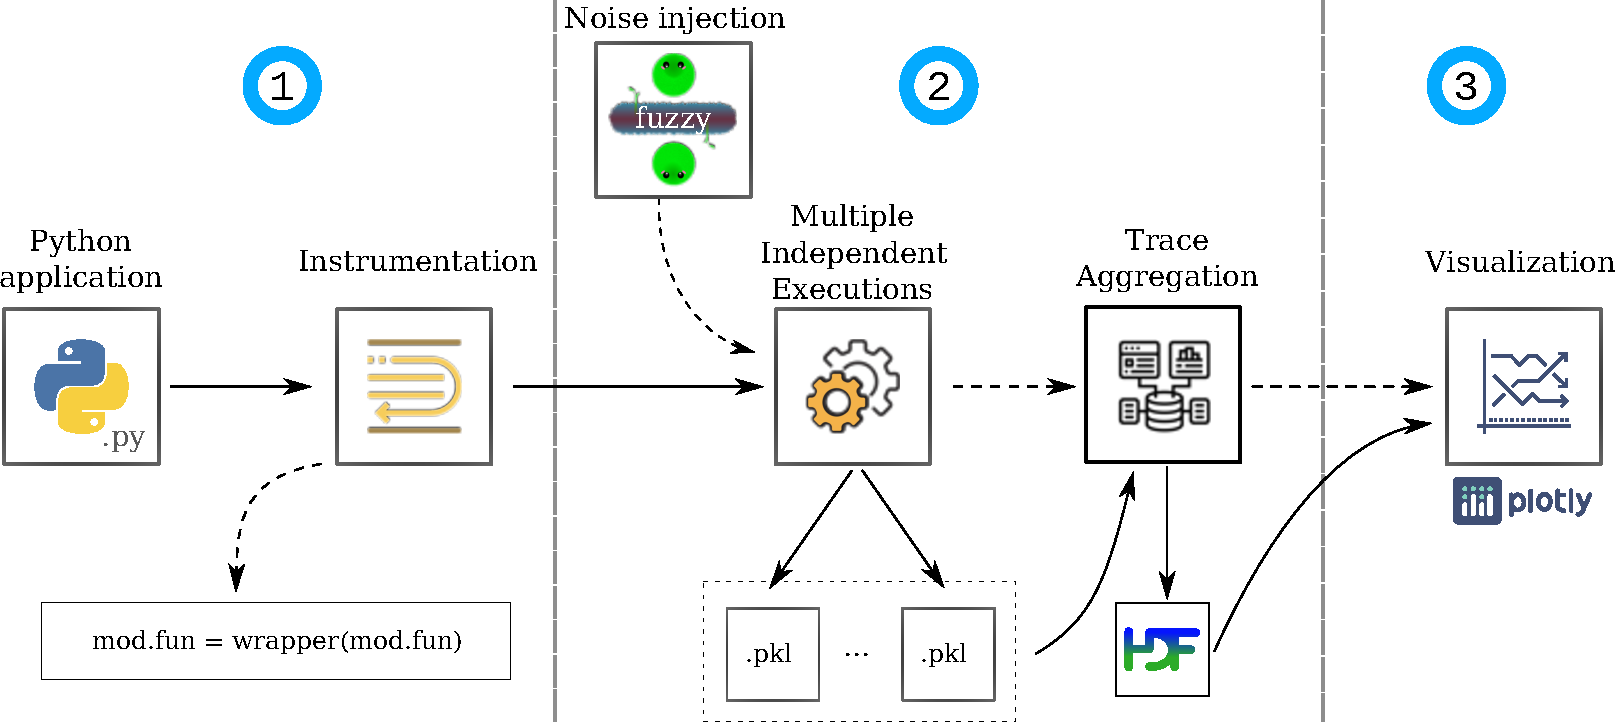
\includegraphics[width=0.75\linewidth]{figure/workflow.pdf}
    \caption{Pytracer workflow
        % \gkmod{}{Note: replace "Execution" with "Multiple Independent
        % Executions", and maybe move it to be between the gears and the pkl
        % files.}
    }
    \label{fig:workflow}
\end{figure*}

\subsection{Python code instrumentation}

%\tristan{``Instrumentation" should appear in Figure 1}


\pytracer dynamically instruments Python modules without requiring source code
modifications in the application. To do so, it creates a new, instrumented
version of each module that preserves its original attributes so that the
application can transparently use it.
% \gkmod{}{Note: this form of monkey patching is basically global and
% transparent decorating, right?} \Yohan{Yes}
By default, \pytracer instruments all the attributes in a given module except
the special ones of the form \texttt{\_\_*\_\_}, which is common for reserved
Python methods. However, some attributes are not writable. In this case,
\pytracer \remove{preservers} \add{preserves} the original attributes and warns
the user. The user can also restrict the list of traced attributes through an
inclusion/exclusion mechanism. The main advantage of this instrumentation
approach is the lack of required modification in the application source code, in
contrast with \remove{decorator-based approaches} \add{a decorator-based
    approach~\mbox{\cite{hunt2019decorators}}}. In addition, this technique is
scalable and applicable in read-only environments such as Singularity containers
or HPC clusters.





\subsubsection{Intercepting module import}

Python loads modules through an import mechanism triggered by the
\texttt{import} keyword that involves two objects: \texttt{finders} and
\texttt{loaders}. \texttt{Finders} search for packages (or
namespaces\footnote{Python distinguishes between \texttt{regular} and
    \texttt{namespace} packages. A regular package is a directory that contains a
    \_\_init\_\_.py file and potentially subdirectories (sub-packages) that contain
    themselves a \texttt{\_\_init\_\_.py} file and so on recursively. The package
    hierarchy follows those of the directory. Namespace packages introduced in
    Python 3.3 (\href{https://www.python.org/dev/peps/pep-0420/}{PEP 420}) do not
    contain an \_\_init\_\_.py file and allow for flexible directory structures.
    Hence, parts of the package can be located in zip files, on the network, or in
    separated directories. There are no functional differences between both types of
    packages.}) on the local storage --- such as standard packages installed through
the pip package manager --- or on a distant server. \texttt{Finders} do not load
modules. Instead, they return a specification (\texttt{spec} object) that
includes information on where to find and how to load modules. \texttt{Loaders}
create module objects, initialize them, and fill import-related attributes such
as \texttt{\_\_spec\_\_}. \texttt{Loaders} then execute modules and populate
their namespace. Finally, modules are bound to their import name in the
\texttt{sys.modules} dictionary.


Python supports custom \texttt{finder} classes registered in the
\texttt{sys.meta\_path} list. When Python encounters an \texttt{import}
statement, it first looks for an existing binding in \texttt{sys.modules} and
then iterates over the \texttt{finder} classes in the \texttt{sys.meta\_path}
list until it finds the module. \pytracer adds a custom \texttt{finder} class at
the head of \texttt{sys.meta\_path} that intercepts the module import and
creates the module with a custom \texttt{loader} class.

\pytracer's \texttt{loader} class first loads the original module, then copies
it as a new instance of the \texttt{ModuleType} class. It then calls the
appropriate instrumentation function for each attribute depending on its type
(function, class, or instances) and replaces the original module in the
\texttt{sys.modules} map with the instrumented version. Finally, it updates all
existing references to the original module contained in the global symbol table.
As a result, the application will transparently call the instrumented module.

\subsubsection{Instrumenting module functions}

\remove{Listings~\mbox{\ref{fig:wrapper_creation}} and~\mbox{\ref{fig:generic_wrapper}} show
    \mbox{\pytracer}'s function instrumentation mechanism.}
For each function to instrument, \pytracer's \texttt{loader} class creates a
wrapper function, dynamically compiles it with the \texttt{compile} builtin
function, and substitutes it for the original module function.  Although simple,
this technique does not apply to callable class instances, i.e., class instances
that have a \texttt{\_\_call\_\_} attribute and are not of type
\texttt{FunctionType}. Indeed, applying the wrapper technique would 1) modify
the type of the class instance to \texttt{FunctionType}, which could cause
syntax and semantic errors, and 2) mask class attributes, leading to
\texttt{AttributeError} exceptions. \pytracer overrides the
\texttt{\_\_call\_\_} attribute with the wrapper function when possible to
overcome this issue. When the \texttt{\_\_call\_\_} attribute is not writable,
Pytracer does not instrument the class and returns a warning. 

\subsubsection{Instrumenting classes}

\pytracer instruments classes by wrapping their callable attributes as described
previously. This instrumentation preserves class types, which avoids type
mismatches in the instrumented application. However, classes that describe
particular base types and NumPy's universal functions (class \texttt{ufunc})
contain read-only attributes that cannot be instrumented. By default, \pytracer
returns a warning when it encounters such classes. 

\subsubsection{Instrumenting class instances}

\pytracer automatically instruments class instances since it instruments
classes. However, it cannot instrument or instantiate classes that have
read-only attributes --- in particular class \texttt{ufunc}, --- which is
problematic given their pervasiveness in scientific computing. In particular,
NumPy's universal functions include vectorized elementary mathematical and other
prevalent functions. Universal functions are implemented in C, which prevents
their modification.

To overcome this issue, \pytracer wraps the class instance into a transparent
wrap class (\texttt{twc}) that overloads 1) function
\texttt{\_\_getattribute\_\_}, called when an instance attribute is accessed ---
instrumented to return the attributes from the original class, and 2) function
\texttt{\_\_call\_\_}, used when an instance behaves like a function through the
() operator --- instrumented with function \texttt{generic\_wrapper}. The
\texttt{twc} returns the queried attribute of the instance instead of returning
its attributes, allowing transparent access to the instance.  Finally, \pytracer
overloads the builtin \texttt{type} function to preserve the type of the wrapped
instance.

\subsubsection{Instrumenting iterators}

In functional programming, iterators traverse containers lazily, meaning that
the next element in the sequence is only computed when the application uses it.
This technique allows for the manipulation of virtually infinite sequences with
finite memory. However, it implies that no complete mapping of the container
returned by an iterator exists in memory since the application computes each
element on the fly. Therefore, iterators are not serializable which implies that
\pytracer cannot save them to output traces. A workaround would be to convert
iterators into explicit containers, however, this would increase the memory
footprint significantly. \pytracer, therefore, does not instrument non-builtin
iterators. 

\subsection{Detecting numerical instabilities}

\pytracer detects numerical instabilities by computing summary statistics across
multiple executions perturbed with numerical noise. While \pytracer's
instrumentation, trace aggregation, and visualization work with various types of
numerical noise, we experimented primarily with Monte-Carlo Arithmetic (MCA) as
it is an accurate model for floating-point errors~\addCite{\cite{verificarlo}}.

\subsubsection{Noise injection}
\label{sec:fuzzy}

Three  main  approaches  exist  to  detect  numerical  instabilities:
stochastic  arithmetic,  uncertainty  or  sensitivity analysis [23], and random
seed analysis [11].  \add{PyTracer is agnostic to the noise model used and can therefore
be used for all these methods}.  For our use cases, we focus on stochastic
arithmetic since it does not make any assumption about the noise model, in
contrast to sensitivity analysis\add{.}

Stochastic arithmetic leverages randomness to estimate numerical instabilities
coming from the use of floating-point representations. The main idea is to treat
round-off errors as random variables and characterize them statistically. Monte 
Carlo Arithmetic (MCA)~\cite{parker1997monte} uses this principle by introducing
two improvements: (i) a virtual precision parameter, allowing to simulate
reduced working precision, and (ii) different perturbation modes to introduce
perturbations on function inputs or output. MCA replaces each floating-point
number $x$ with a stochastic counterpart computed as:
\[
    inexact(x) =  x + \beta^{e_x - t}\xi
\]
where $\beta$ is the number base, $e_x$ is the magnitude of $x$, $t$ the virtual
precision and $\xi \in (-\frac{1}{2},\frac{1}{2})$ is a random uniform variable.
Virtual precision allows for the simulation of reduced working precision.
\add{In our experiments, we used MCA in Random Rounding (RR) mode, which
    simulates roundoff errors by applying function $inexact$ only to the
    output returned by a function. The Precision Bounding (PB) mode can
    identify other types of instabilities, in particular catastrophic
    cancellations, however, it is more difficult to apply to large code bases
    as it often leads to execution errors that require human intervention.}

Stochastic arithmetic quantifies numerical error using the number of significant
digits $s$ estimated among the sampled values. A common formula to determine
this number from MCA samples is presented in~\cite{parker1997monte}:
\begin{equation}
    s = -\log_{\beta}{ \left| \dfrac{\sigma}{\mu} \right|} \label{eq:sig-digits}
\end{equation}
where $\mu$ and $\sigma$ are the sample mean and standard deviation of a
variable sampled with MCA. \add{This can be seen as the ratio signal over noise.}
Sohier et al.~\cite{sohier2021confidence} recently provided a generalization of
this formula to include confidence intervals.

We enabled MCA in Python programs via Verificarlo~\cite{verificarlo}, a
clang-based compiler~\cite{lattner2008llvm} that replaces floating-point
operations by a generic call to a configurable floating-point model. Several
floating-point models are
available~\cite{chatelain2019automatic,chatelain2019outils}, also called
backends. \pytracer leverages Fuzzy~\cite{kiar2020comparing}, a collection of
software tools compiled with Verificarlo. In particular, Fuzzy provides
MCA-instrumented versions of the Python interpreter as well as the BLAS, LAPACK,
NumPy, SciPy, and scikit-learn libraries, which enables MCA for a wide range of
existing scientific Python programs. Fuzzy is available in Verificarlo's GitHub
organization at
\href{https://github.com/verificarlo/fuzzy}{\url{github.com/verificarlo/fuzzy}}.


\add{Monte Carlo Arithmetic samples the floating-point variability of a given
    program, and hence the more MCA repetitions we have, the more accurate the
    distribution will be. In theory, an infinite number of MCA repetitions
    should give the exact distribution. While in practice low sample sizes (3 to 30)
    can give good estimates, the issue is to capture ``rare events" that could make the
    computation strongly diverge from the mean. Determining the number of
    MCA samples to use for a given instrumented code is still an open research question. 
    Recent theoretical works}~\cite{sohier2021confidence}
\add{on the estimation of significant digits allow computing an associated
    confidence interval depending on the sample size and the underlying distribution.}

\subsubsection{Trace format}

\pytracer stores traces in the pickle format, a binary format to serialize
Python objects. The main advantages of the pickle format compared to other
serialization approaches such as marshal or JSON are its ability to serialize
most Python objects and its native compression.  In addition, pickle writes
Python objects sequentially, which preserves the temporal ordering required by
subsequent trace analyses.

Traces store numerical values at the granularity of function calls. When the
application invokes a function, \pytracer saves a call input object containing
contextual information (function's name, module's function, stacktrace) and the
values of the function arguments. When the function returns, \pytracer saves a
similar call output object containing the returned value. 


\subsubsection{Trace aggregation}

Once traces are available, \pytracer sequentially parses them and computes the
mean, standard deviation, and the number of significant digits (as in
Equation~\ref{eq:sig-digits}) of all saved values. \pytracer saves these summary
statistics in an HDF5 file, a hierarchical format that facilitates visual
browsing since only required information are loaded when requested by the user.
This operation critically relies on the ordering of call input and output
objects in the traces. Therefore, it assumes that the application is
single-threaded and that the control flow does not depend on a random state.
\add{Therefore, \mbox{\pytracer} cannot merge traces resulting from different
    control flow paths and will stop the parsing when encountering such a situation.}

\begin{figure*}
    \centering
    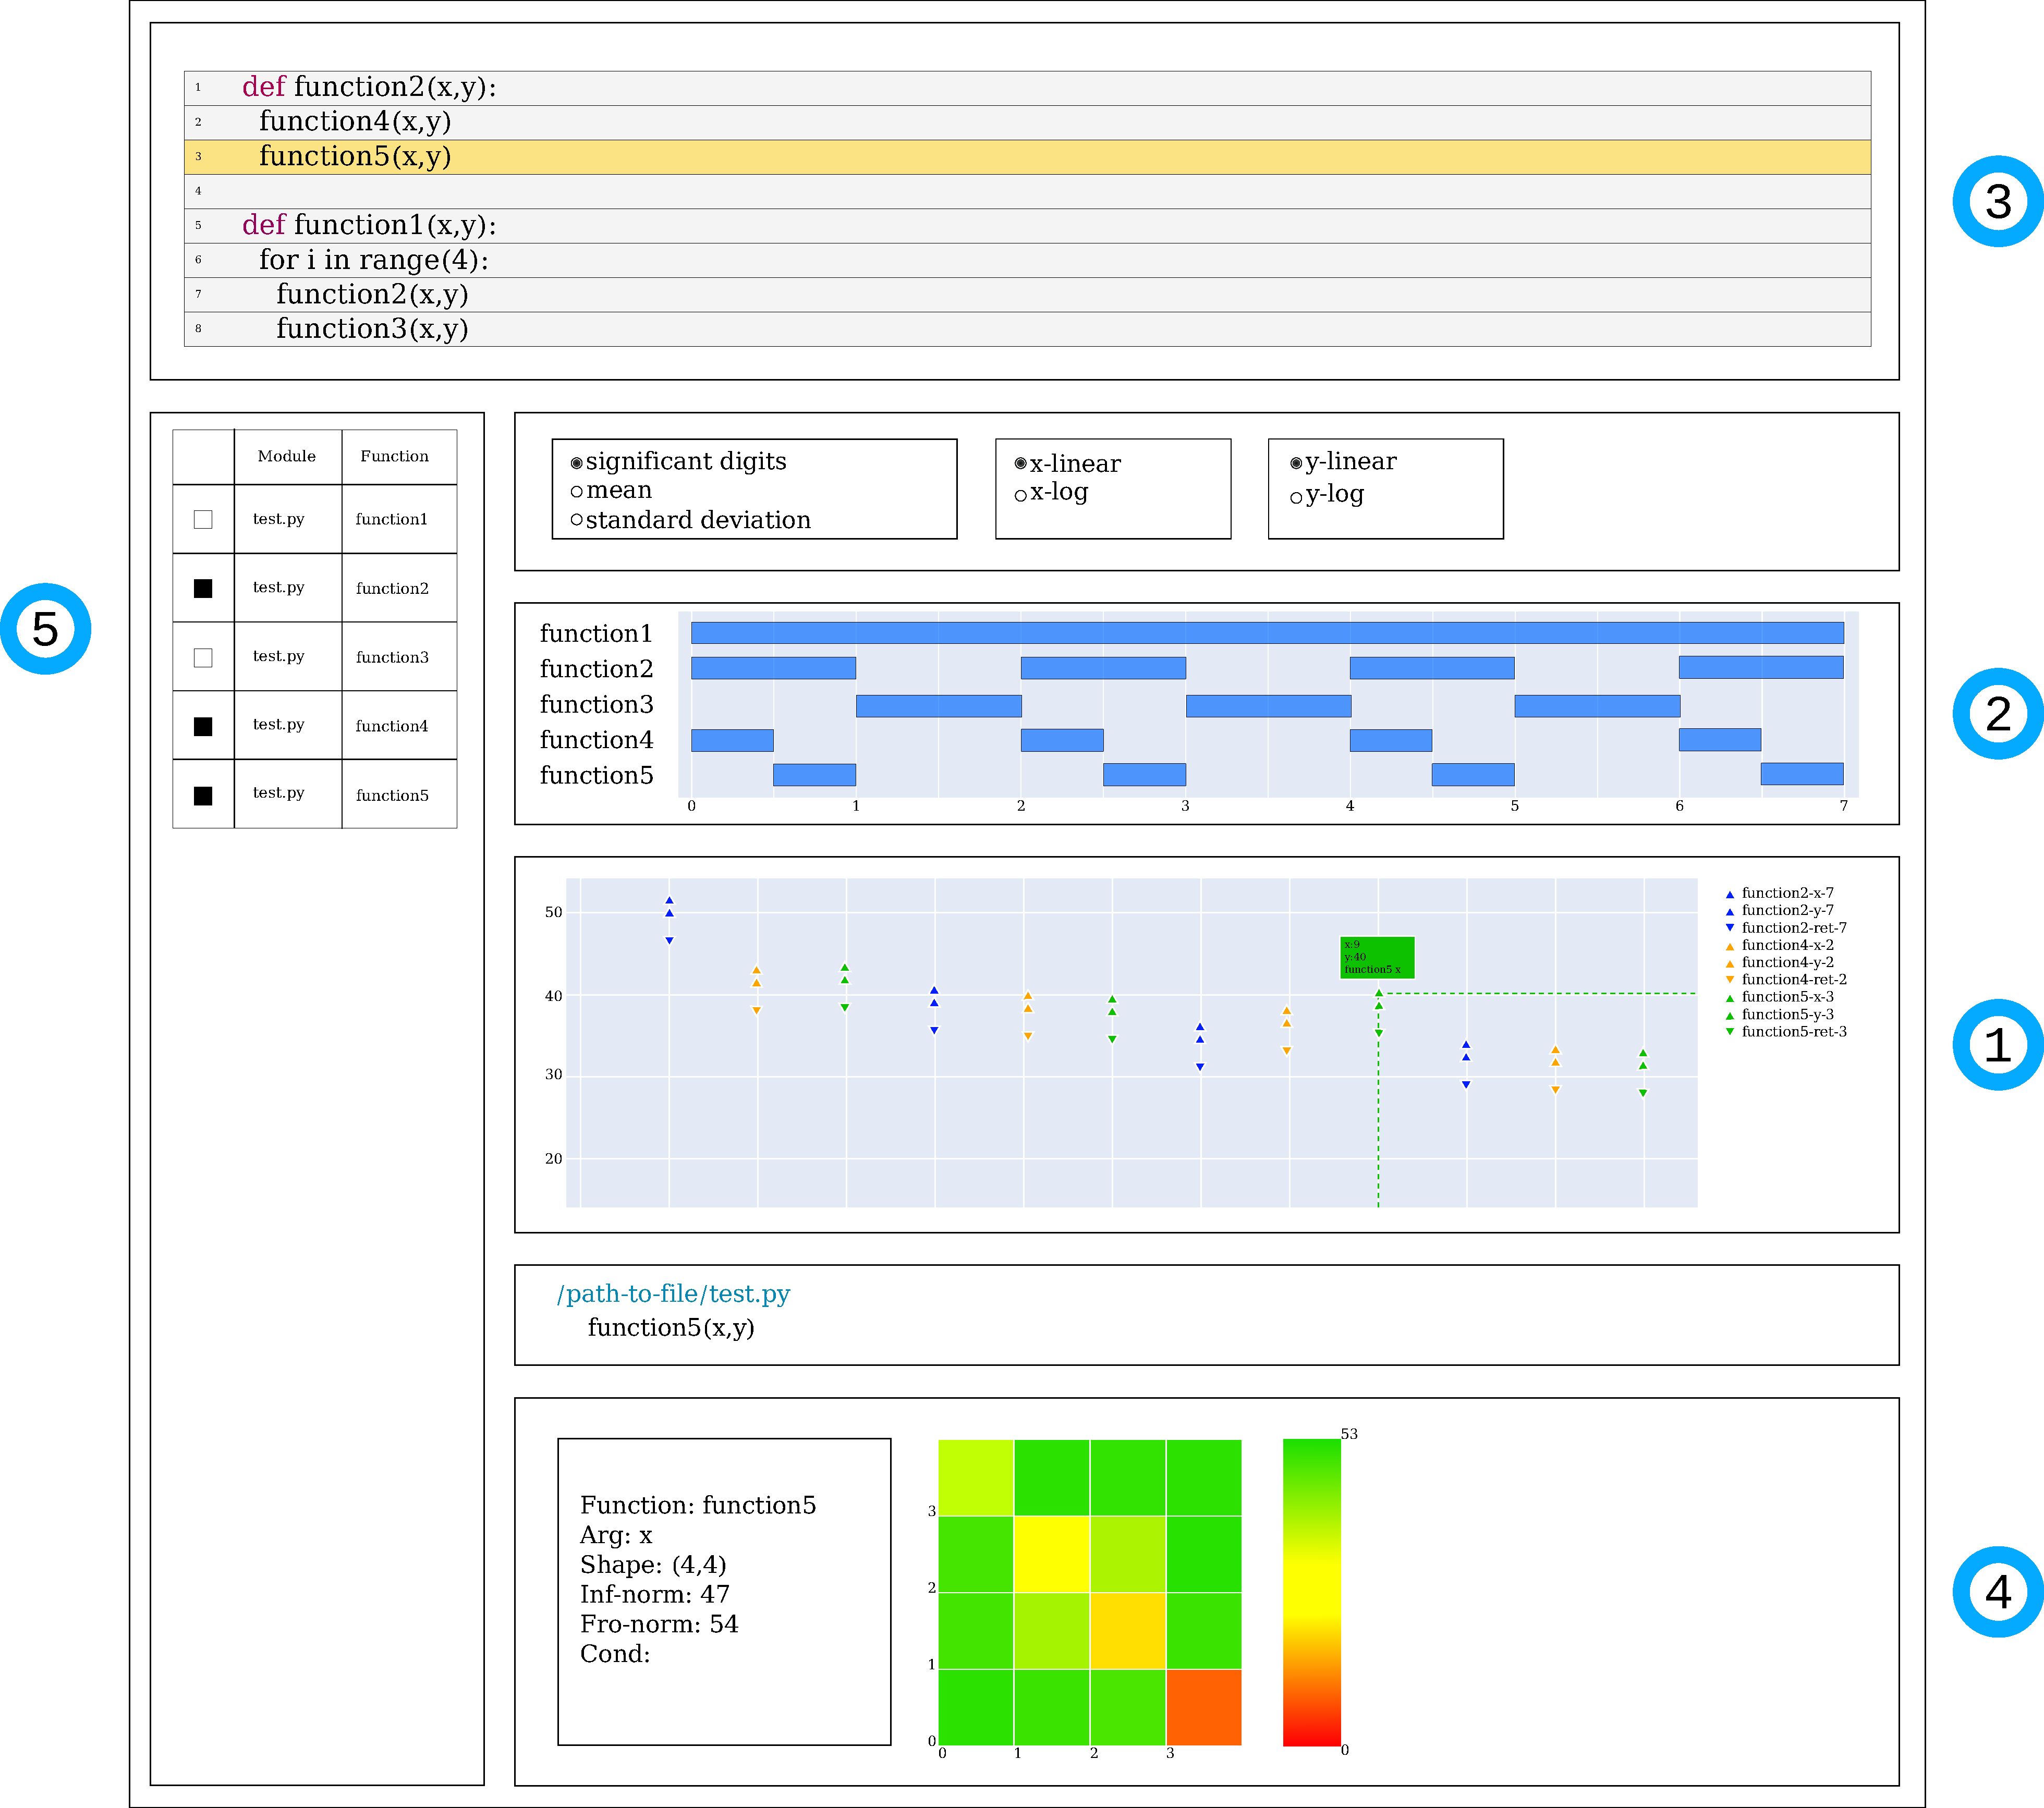
\includegraphics[width=0.75\linewidth]{figure/pytracer_layout.pdf}
    \caption{Pytracer visualization layout.}
    \label{fig:visu-layout}
\end{figure*}


To aggregate traces, \pytracer successively unpickles call objects in each
trace, checks that the call objects refer to the same function and stacktrace,
and terminates the parsing otherwise. PyTracer stores function arguments or
returned values in a NumPy array for each matching call object to compute
statistics. For compound objects such as tuples, dictionaries, or objects, it
recursively parses the fields until finding numeric types or NumPy arrays of
numeric types.

\subsection{Interactive visualization}
The third main component of \pytracer is its interactive trace visualizer built
with Plotly Dash~\cite{plotly}, a Python framework for web visualization. Plotly
Dash abstracts the low-level details of web applications in a highly
customizable development interface allowing to offload heavy computations to a
server if necessary. Figure~\ref{fig:visu-layout} presents the general layout of
the \pytracer visualizer, divided into five sub-components:
\begin{enumerate}
    \item Timeline view: This view displays the values of each input and output
          for a given function at a given invocation. By default, \pytracer
          shows the number of significant digits computed across the traces. The
          mean and standard deviation across perturbed samples are also
          available. The visualizer uses an upper triangle for inputs and a
          lower triangle for outputs. \pytracer internally represents all values
          as NumPy arrays. In the case of non-scalar values or types that cannot
          be trivially cast into NumPy arrays, \pytracer splits the value into
          several variables. Hence, \pytracer will transform a class containing
          $n$ floating-point parameters into $n$ variables. Each variable is
          prefixed with the original value and postfixed with the name of the
          parameter. Finally, non-scalar values (vectors or matrices) are
          represented by their average and can be inspected with the Zoom view
          (see below).
    \item Gantt chart view: This view displays the call graph as a Gantt chart
          representing the instrumented functions. Each function call is
          represented with a bar. The time overlaps reflect the caller/callee
          relation. For example, in the figure, \texttt{function1} calls
          \texttt{function2} that itself calls \texttt{function4} and
          \texttt{function5}. This view provides insights on the calling context
          for each function, which may influence numerical stability.
    \item  Source code view: This view displays a local snapshot of the source
          code file of the variable hovered in the timeline view.
    \item Zoom view: This view provide details about non-scalar values. For
          example, a matrix may have instabilities around its diagonal but not
          in other regions. The visualizer also provides additional metrics such
          as array shape, infinite norm, or condition number.
    \item  Functions list view: This view allows the user to select the
          functions plotted in the timeline view.
\end{enumerate}

\section{Results}

We evaluated \pytracer on two widely-used Python libraries:
SciPy~\cite{virtanen2020scipy}, the main library for scientific computing in
Python, and  scikit-learn~\cite{pedregosa2011scikit}, a reference
machine-learning framework that implements a wide range of state-of-the-art
algorithms. For each library, we executed the software examples provided in
their respective GitHub repositories. We traced each example five times, having
activated MCA through Fuzzy in the Python interpreter \add{as well as} BLAS, LAPACK, NumPy,
SciPy, and scikit-learn. \add{These libraries are written in large parts in a 
compiled language other than Python (such as C or Cython) and their execution is not 
perturbed by the sole use of Fuzzy Python. We chose to activate MCA in these libraries 
to provide an overall picture of numerical uncertainty in the tested examples. 
Depending on the use-case of interest, one might choose to use MCA only in 
a subset of these libraries or even just in the Python interpreter.} \add{We
    used MCA in Random Rounding (RR) mode}. We used the default virtual
precision in Verificarlo, namely 24 bits for single-precision floating-point
values and 53 bits for double-precision values, which simulates machine error.
We used Python-3.8.5, NumPy-1.19.1, SciPy-1.5.4, and scikit-learn-0.23.2.

\begin{table*}[]
    \centering
    \normalsize
    \begin{subfigure}[t]{\linewidth}
        \centering
        \begin{tabular}{|lll|c|c|c|}
            \hline
            \multicolumn{3}{|c}{ \multirow{2}{*}{Application} }                 & \multicolumn{3}{|c|}{Random Rounding (RR)}                                                                                                                         \\
            \cline{4-6}
                                                                                &                                                                           &                                                          & trace  & parse    & sigbits \\
            \hline
            \multicolumn{1}{|c|}{ \multirow{20}{2em}{ \rotatebox{90}{SciPy} } } & 
            \multicolumn{1}{c|}{ \multirow{3}{2em}{ \rotatebox{90}{FFT} }}      & \discreteCosineRF                                                         & \valid                                                   & \valid & \s{52}             \\ 
            \multicolumn{1}{|c|}{}                                              & \multicolumn{1}{c|}{}                                                     & \fftOneDRf                                               & \valid & \valid   & 41      \\
            \multicolumn{1}{|c|}{}                                              & \multicolumn{1}{c|}{}                                                     & \fftTwoDRf                                               & \valid & \valid   & \s{52}  \\
            \cline{2-6}
            \multicolumn{1}{|c|}{}                                              & \multicolumn{1}{c|}{  \multirow{5}{*}{ \rotatebox{90}{Interpolation} } }
                                                                                & \interOneDRf                                                              & \valid                                                   & \valid & 51                 \\
            \multicolumn{1}{|c|}{}                                              & \multicolumn{1}{c|}{}                                                     & \multiRf                                                 & \valid & \valid   & \s{51}  \\
            \multicolumn{1}{|c|}{}                                              & \multicolumn{1}{c|}{}                                                     & \bsplineRf                                               & \valid & \valid   & 10      \\
            \multicolumn{1}{|c|}{}                                              & \multicolumn{1}{c|}{}                                                     & \splineOneDRf                                            & \valid & \cross   & \s{52}  \\
            \multicolumn{1}{|c|}{}                                              & \multicolumn{1}{c|}{}                                                     & \splineTwoDRf                                            & \valid & \valid   & 10      \\
            \cline{2-6}
            \multicolumn{1}{|c|}{}                                              & \multicolumn{1}{c|}{ \multirow{12}{2em}{ \rotatebox{90}{Optimization} } }
                                                                                & \bfgsRf                                                                   & \valid                                                   & \valid & \s{48}             \\
            \cline{3-6}
            \multicolumn{1}{|c|}{}                                              & \multicolumn{1}{c|}{}                                                     & \globalRf                                                & \valid & \cross   & 17      \\
            \multicolumn{1}{|c|}{}                                              & \multicolumn{1}{c|}{}                                                     & | SHGO\footnote{Simplicial Homology Global Optimization} & \na    & \na      & \s{25}  \\
            \multicolumn{1}{|c|}{}                                              & \multicolumn{1}{c|}{}                                                     & | Dual Annealing                                         & \na    & \na      & 4       \\
            \multicolumn{1}{|c|}{}                                              & \multicolumn{1}{c|}{}                                                     & | Differential Evolution                                 & \na    & \na      & \s{0}   \\
            \multicolumn{1}{|c|}{}                                              & \multicolumn{1}{c|}{}                                                     & | Basin Hopping                                          & \na    & \na      & 40      \\
            \multicolumn{1}{|c|}{}                                              & \multicolumn{1}{c|}{}                                                     & | SHGO Sobol                                             & \na    & \na      & \s{45}  \\
            \cline{3-6}
            \multicolumn{1}{|c|}{}                                              & \multicolumn{1}{c|}{}                                                     & \slsqpRf                                                 & \valid & \valid   & 45      \\
            \multicolumn{1}{|c|}{}                                              & \multicolumn{1}{c|}{}                                                     & \lsmRf                                                   & \valid & \valid   & \s{48}  \\
            \multicolumn{1}{|c|}{}                                              & \multicolumn{1}{c|}{}                                                     & \nelderRf                                                & \valid & \valid   & 44      \\
            \multicolumn{1}{|c|}{}                                              & \multicolumn{1}{c|}{}                                                     & \ncgRf                                                   & \valid & \valid   & \s{48}  \\
            \multicolumn{1}{|c|}{}                                              & \multicolumn{1}{c|}{}                                                     & \rootRf                                                  & \valid & \cross   & 52      \\
            \multicolumn{1}{|c|}{}                                              & \multicolumn{1}{c|}{}                                                     & \rootLargRf                                              & \valid & \cross   & \s{29}  \\
            \multicolumn{1}{|c|}{}                                              & \multicolumn{1}{c|}{}                                                     & \rootLargePredRf                                         & \valid & \cross   & 42      \\
            \multicolumn{1}{|c|}{}                                              & \multicolumn{1}{c|}{}                                                     & \trustExactRf                                            & \valid & \valid   & \s{48}  \\
            \multicolumn{1}{|c|}{}                                              & \multicolumn{1}{c|}{}                                                     & \trustTruncRf                                            & \valid & \valid   & 48      \\
            \multicolumn{1}{|c|}{}                                              & \multicolumn{1}{c|}{}                                                     & \trustNCGRf                                              & \valid & \valid   & \s{52}  \\
            \hline
            \multicolumn{2}{|c|}{ \multirow{20}{2em}{ \rotatebox{90}{Scikit-learn} } }
                                                                                & \AdaboostRf                                                               & \valid                                                   & \valid & 48                 \\
            \cline{3-6}
            \multicolumn{2}{|c|}{}                                              & \brrRf                                                                    & \valid                                                   & \valid & \s{25}             \\
            \multicolumn{2}{|c|}{}                                              & | $1^{st}$ dataset                                                        & \na                                                      & \na    & 25                 \\
            \multicolumn{2}{|c|}{}                                              & | $2^{nd}$ dataset                                                        & \na                                                      & \na    & \s{nan}            \\
            \cline{3-6}
            \multicolumn{2}{|c|}{}                                              & \onlineClassifierComparisonRf                                             & \valid                                                   & \valid & 20                 \\
            \multicolumn{2}{|c|}{}                                              & \kmeansRf                                                                 & \valid                                                   & \valid & \s{52}             \\
            \multicolumn{2}{|c|}{}                                              & \covarianceRf                                                             & \valid                                                   & \cross & 48                 \\
            \multicolumn{2}{|c|}{}                                              & \decisionRf                                                               & \valid                                                   & \valid & \s{50}             \\
            \multicolumn{2}{|c|}{}                                              & \digitsRf                                                                 & \valid                                                   & \valid & 52                 \\
            \multicolumn{2}{|c|}{}                                              & \faceRf                                                                   & \cross                                                   & \valid & \s{-}              \\
            \multicolumn{2}{|c|}{}                                              & \penaltyRf                                                                & \valid                                                   & \valid & -                  \\
            \multicolumn{2}{|c|}{}                                              & \lassoRf                                                                  & \valid                                                   & \valid & \s{48}             \\
            \multicolumn{2}{|c|}{}                                              & \hyperplaneRf                                                             & \valid                                                   & \valid & 3                  \\
            \multicolumn{2}{|c|}{}                                              & \mnistRf                                                                  & \valid                                                   & \valid & \s{43}             \\
            \multicolumn{2}{|c|}{}                                              & \multitaskRf                                                              & \valid                                                   & \valid & 50                 \\
            \multicolumn{2}{|c|}{}                                              & \ompRf                                                                    & \valid                                                   & \valid & \s{52}             \\
            \multicolumn{2}{|c|}{}                                              & \pcaRf                                                                    & \valid                                                   & \valid & 48                 \\
            \cline{3-6}
            \multicolumn{2}{|c|}{}                                              & \robustRf                                                                 & \valid                                                   & \valid & \s{50}             \\
            \multicolumn{2}{|c|}{}                                              & | Linear                                                                  & \na                                                      & \na    & 48                 \\
            \multicolumn{2}{|c|}{}                                              & | RANSAC                                                                  & \na                                                      & \na    & \s{50}             \\
            \cline{3-6}
            \multicolumn{2}{|c|}{}                                              & \toyRf                                                                    & \valid                                                   & \valid & 35                 \\
            \cline{3-6}
            \multicolumn{2}{|c|}{}                                              & \svmRf                                                                    & \valid                                                   & \valid & \s{43.5}           \\
            \multicolumn{2}{|c|}{}                                              & | Non-weighted                                                            & \na                                                      & \na    & 43                 \\
            \multicolumn{2}{|c|}{}                                              & | Weighted                                                                & \na                                                      & \na    & \s{44}             \\
            \cline{3-6}
            \multicolumn{2}{|c|}{}                                              & \tomographyRf                                                             & \valid                                                   & \cross & -                  \\
            \multicolumn{2}{|c|}{}                                              & \weightedRf                                                               & \valid                                                   & \valid & \s{44}             \\
            \hline
        \end{tabular}
    \end{subfigure}
    \caption{\pytracer execution summary on SciPy and Scikit-learn examples.
        % \tristan{Replace FFT with SciPy FFT, Interpolation with SciPy
        % Interpolation and Optimization with SciPy Optimization, or add a SciPy
        % header to these rows.} \tristan{Nitpick: you could add a color scheme
        % to sigbits (for instance shades of blue), to make the column more
        % easily readable.} \\
        \emph{trace}: outcome of \pytracer tracing, \emph{parse}: outcome of
        \pytracer trace parsing and aggregation, \emph{result}: precision for
        main outputs in significant bits. \valid: successful run, \remove{\warn: error
            from invalid noise injection,} \cross: numerical error or divergent
        traces. \textit{nan} stands for (\texttt{Not-A-Number}). Example names
        are linked to their source code.}
    \label{tab:pytracer_results_summary}
\end{table*}


\subsection{\pytracer is applicable to reference scientific computating libraries}

Table~\ref{tab:pytracer_results_summary} summarizes \pytracer's outcome on SciPy
and scikit-learn examples. Columns \textit{trace} and \textit{parse} report on
the tracing and aggregation steps with two possible outcomes: 1) green for
success, meaning that the execution ended well and no issues were raised by the
application, and 2) red for numerical error in the application, meaning that the
execution raised a Python error before the end. \remove{, and 3)
    orange for errors due to the Fuzzy noise injection that are
    not considered numerical errors, meaning that the execu-
    tion raised a Python error but due to a perturbation that
    should not have been introduced (i.e. a floating-point value
    representing an integer).}
Overall, the tracing and parsing of SciPy and scikit-learn examples in Random
Rounding mode was entirely successful for 32/40 examples\remove{ and showed an average
    precision loss of 8 bits}. The remaining examples failed due to numerical errors
in the libraries, which we discuss hereafter. 
\remove{The instrumentation with Full MCA is
    more invasive and reduced the number of successful exe-
    cutions to 12/40. Among the 28/40 failed executions, one
    failed due to an actual numerical error (Bayesian Ridge
    Regression example) and the other ones failed due to
    perturbations that should not have been introduced.}

Column \textit{sigbits} in Table~\ref{tab:pytracer_results_summary} summarizes
the precision for the main outputs of SciPy and scikit-learn examples. We
measured the precision in significant bits on the final primary example output
by taking the element-wise mean for non-scalar values and, if the example
produces many outputs, the average value among them. The numerical
quality across all examples varied from 0 to 52, with an average of 44
significant bits. We note that only one example failed due to a
numerical error (\texttt{face\_recognition}
\remove{for RR and \texttt{Bayesian Ridge Regression} for full MCA}).

\noindent \remove{\textbf{3.2 Effect of MCA modes}}

\remove{
    Random Rounding perturbs only the result of a floating-point operation while
    Full MCA perturbs both the inputs and the result. Therefore, Full MCA may
    trigger catastrophic cancellations while Random Rounding only introduces
    round-off errors which generally have a lesser impact. Moreover, Random Rounding
    preserves exact operations --- operations where the result can be exactly
    represented at the virtual precision --- while Full MCA does not.}

\remove{\pytracer can only aggregate traces obtained from the same control flow path. In
    particular, program branches triggered by an unstable floating-point comparison
    lead to different control flows and result in parsing errors. For example,
    comparing a residual error or the distance between two points to a strict
    threshold in an iterative scheme generally results in unstable branches. Full
    MCA even perturbs exact values such as integers represented with floating-point
    values, leading to many execution failures. For instance, the \texttt{fft1}
    example from SciPy raised an \texttt{ValueError: operands could not be broadcast
        together with shapes (601,) (600,)} error due to an array shape mismatch. A
    closer inspection showed that one of the arrays involved in the error was
    created with the NumPy function \texttt{linspace} that itself calls function
    \texttt{arange} (Listing~\ref{fig:pyarray_range_code}). Lines 3174-3178 show
    that the function stores the array size in a floating-point value that will be
    perturbed by Full MCA, as shown in Table~\ref{tab:mca_result_linspace},
    resulting in array sizes that fluctuate between N and N+1. It is worth noting
    that 78\% of execution issues encountered in Full MCA mode instrumentation are
    due to this type of ``typing" errors.  
    Those code regions should not be perturbed by MCA since the injected noise does
    not make sense.}

\subsection{\pytracer supports the profiling of compound data types}

\add{PyTracer supports native floating point formats as well as compound data types,
    such as complex floating point values, N-dimensional arrays and arbitrary Python
    classes.}
Figures~\ref{fig:fft1D_inputs} and~\ref{fig:fft1D_outputs} \add{show the
    visualization of the \texttt{fft\_1D} input and output values. Results are
    complex values encoded in double precision. PyTracer allows visualizing the
    numerical precision of real (blue points) and imaginary (orange points) parts.}
\add{The} top row in Figures~\ref{fig:fft1D_inputs} and~\ref{fig:fft1D_outputs}
show the input mean value while the bottom row shows the standard deviation. The
points with low magnitude in Figure~\ref{fig:fft1D_inputs} correspond to inputs
near 0 when the input of $\sin$ or $\exp$ is close to $k\pi$, $k \in
    \mathbb{Z}$. Indeed, since MCA introduces a slight noise, the result is not
exactly 0. We can see in Figure~\ref{fig:fft1D_inputs} that the maximal noise
introduced by MCA on the inputs is in the order of $10^{-14}$, two orders of
magnitude higher than the $ulp \simeq 10^-16$ for double precision. This slight
noise introduced can be interpreted as white noise on the input signal. We can
see on the bottom row of Figure~\ref{fig:fft1D_outputs} that the frequency noise
is of the same order of of magnitude as the input noise, which is expected. The
two peaks at x=38 and x=562 corresponds to the actual frequencies of the input
signal.

Figure~\ref{fig:spline2d_rr} \add{shows the results of the spline evaluation with
    \texttt{bisplev} from the \texttt{spline\_2D} example. It computes the 2D spline
    interpolation for function $z=(x+y)e^{-6(x^2+y^2)}$, with $(x,y) \in
        [-1,1]\times[-1,1]$. The result is a 2D-array that is natively supported by
    PyTracer. We observe a significant loss of precision in some regions, which follows
    an interesting pattern that could be further investigated.}


\begin{figure}
    \centering
    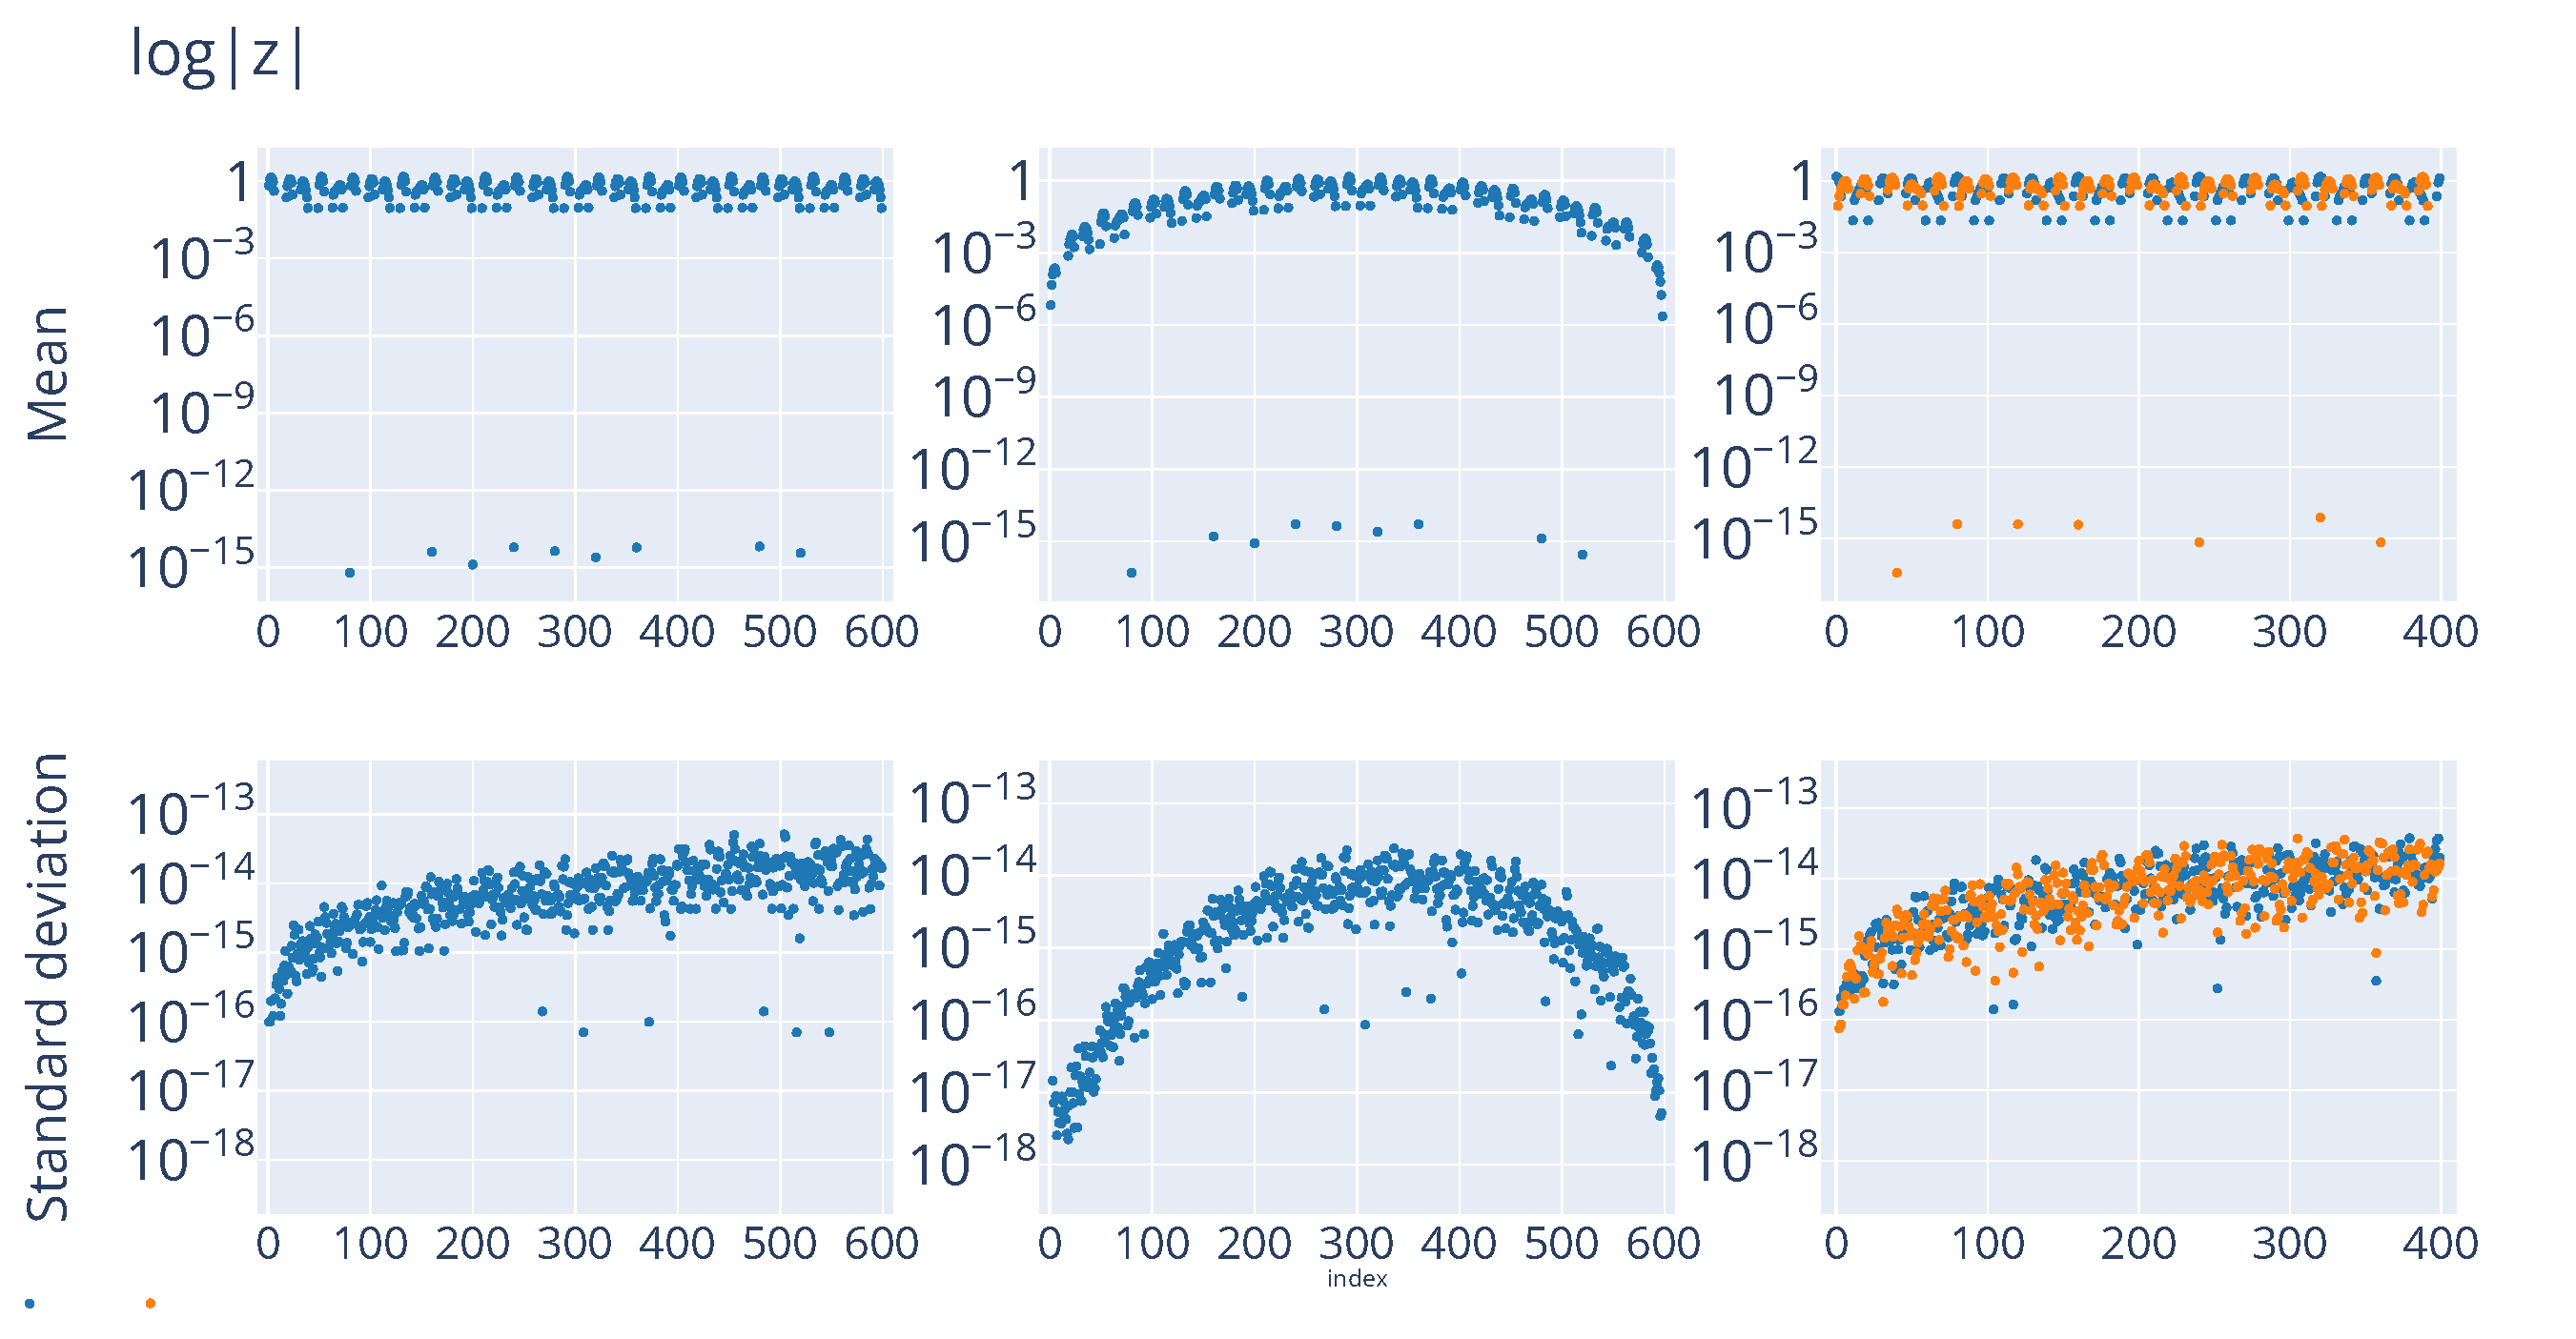
\includegraphics[width=\linewidth]{figure/FFT/fft_x.pdf}
    \caption{Absolute value of the mean and standard deviation values for fft 1D
        inputs within RR mode (log scale). The real part is shown in blue and
        the imaginary part in orange.}
    \label{fig:fft1D_inputs}
\end{figure}

\begin{figure}
    \centering
    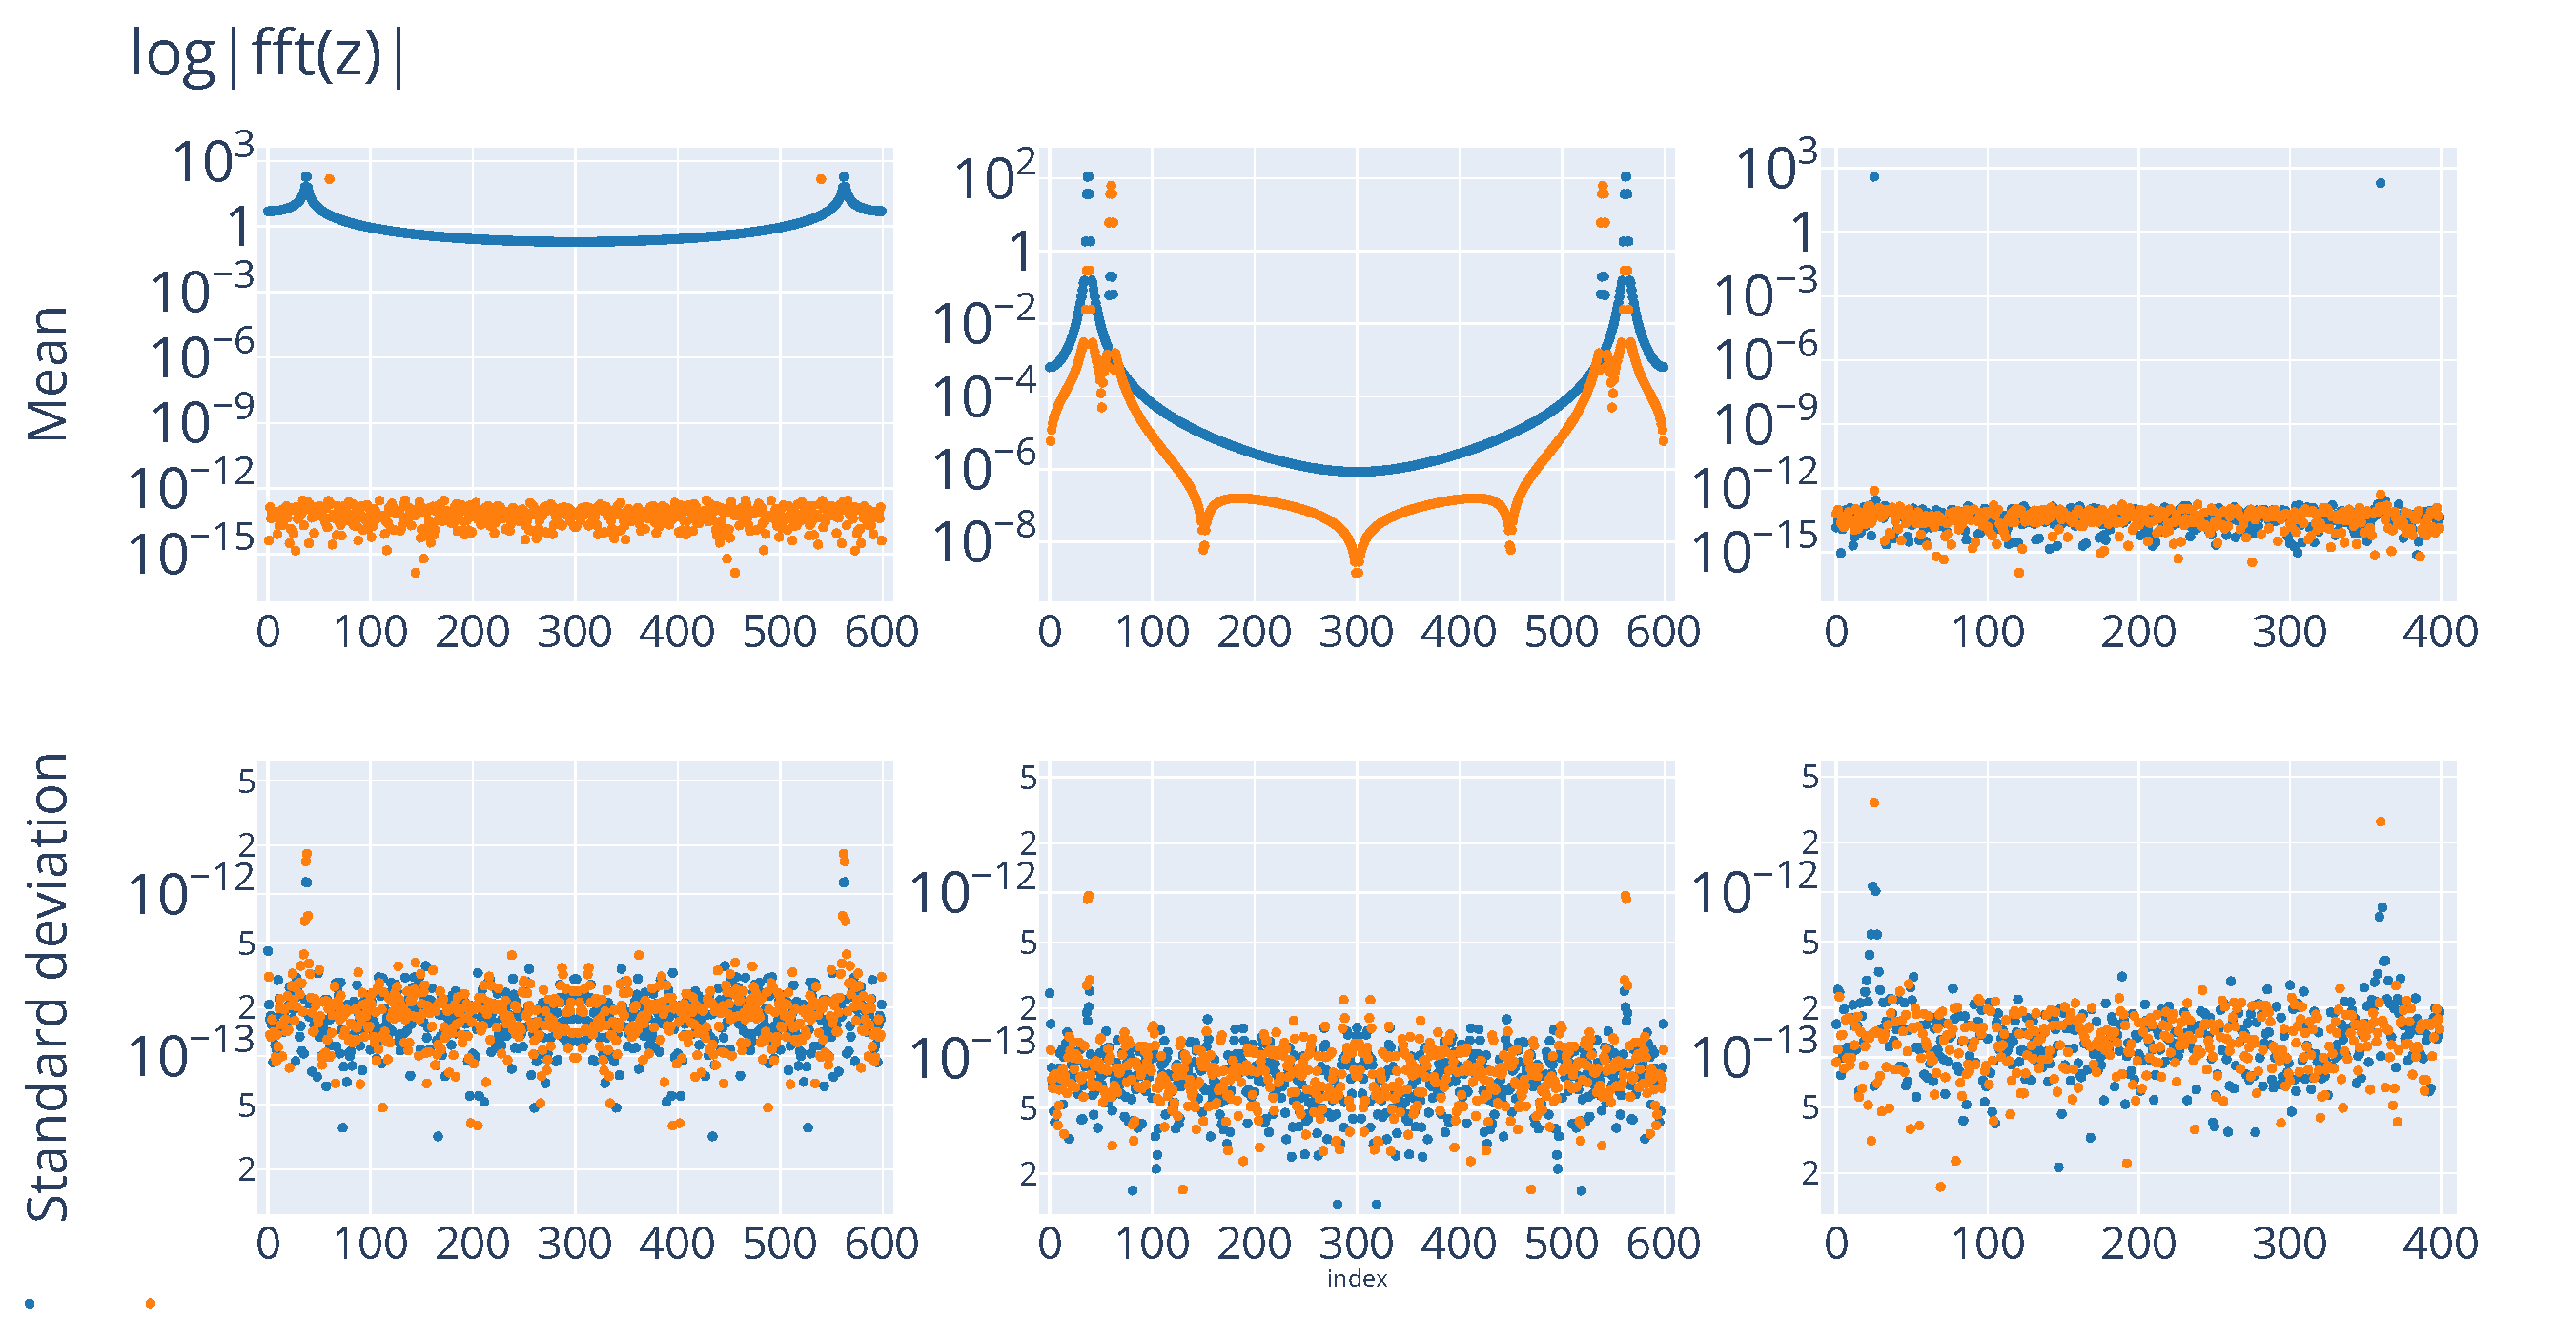
\includegraphics[width=\linewidth]{figure/FFT/fft_y.pdf}
    \caption{Absolute value of the mean and standard deviation values
        for fft 1D outputs within RR mode (log scale).}
    \label{fig:fft1D_outputs}
\end{figure}


\begin{figure*}
    \centering
    \begin{subfigure}{.3\linewidth}
        \centering
        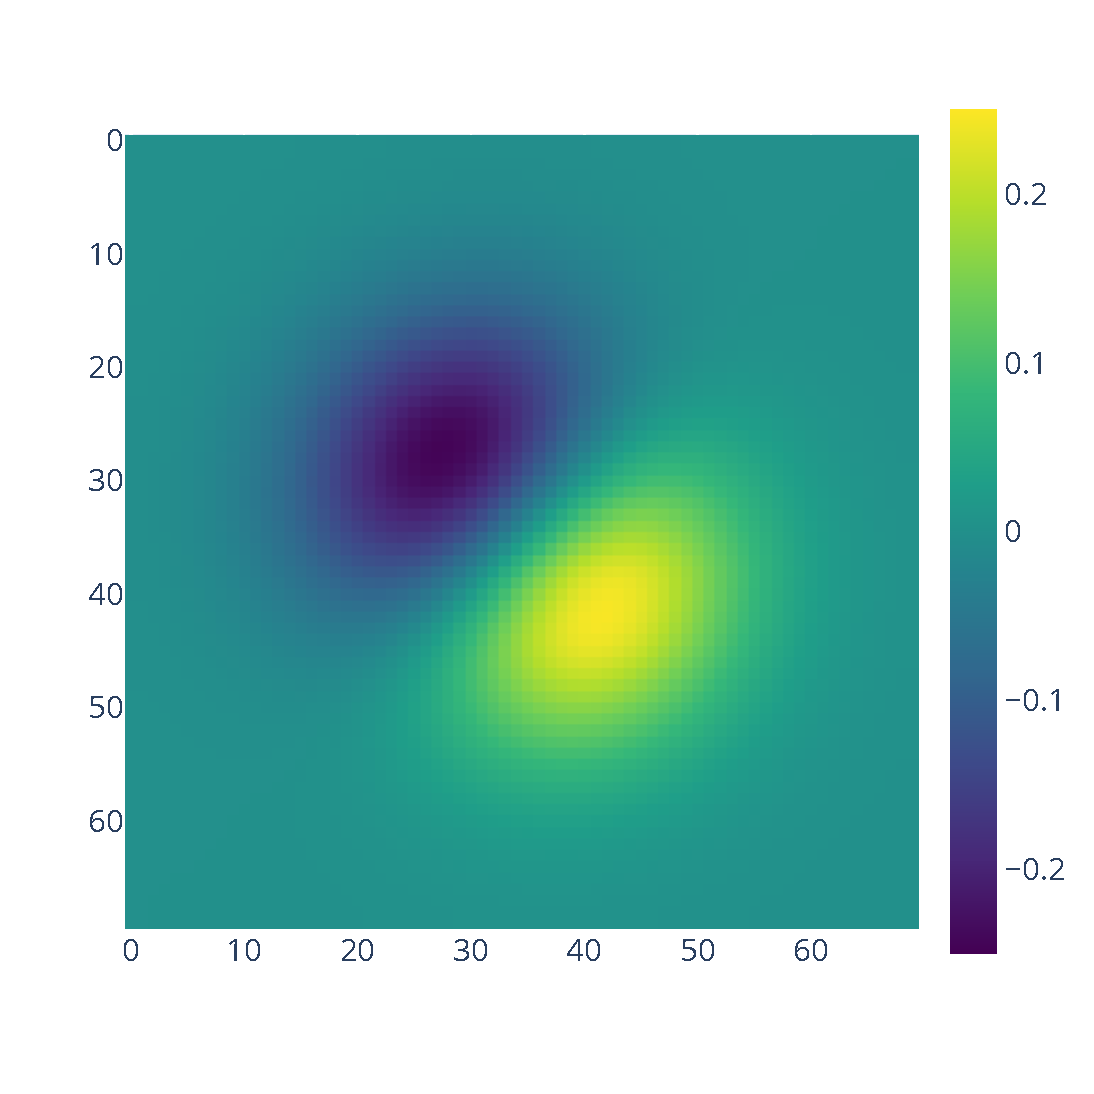
\includegraphics[width=\linewidth]{figure/spline_2d/bisplev_mean.pdf}
        \caption{Mean value}
        \label{fig:bisplev_mean}
    \end{subfigure}
    \begin{subfigure}{.3\linewidth}
        \centering
        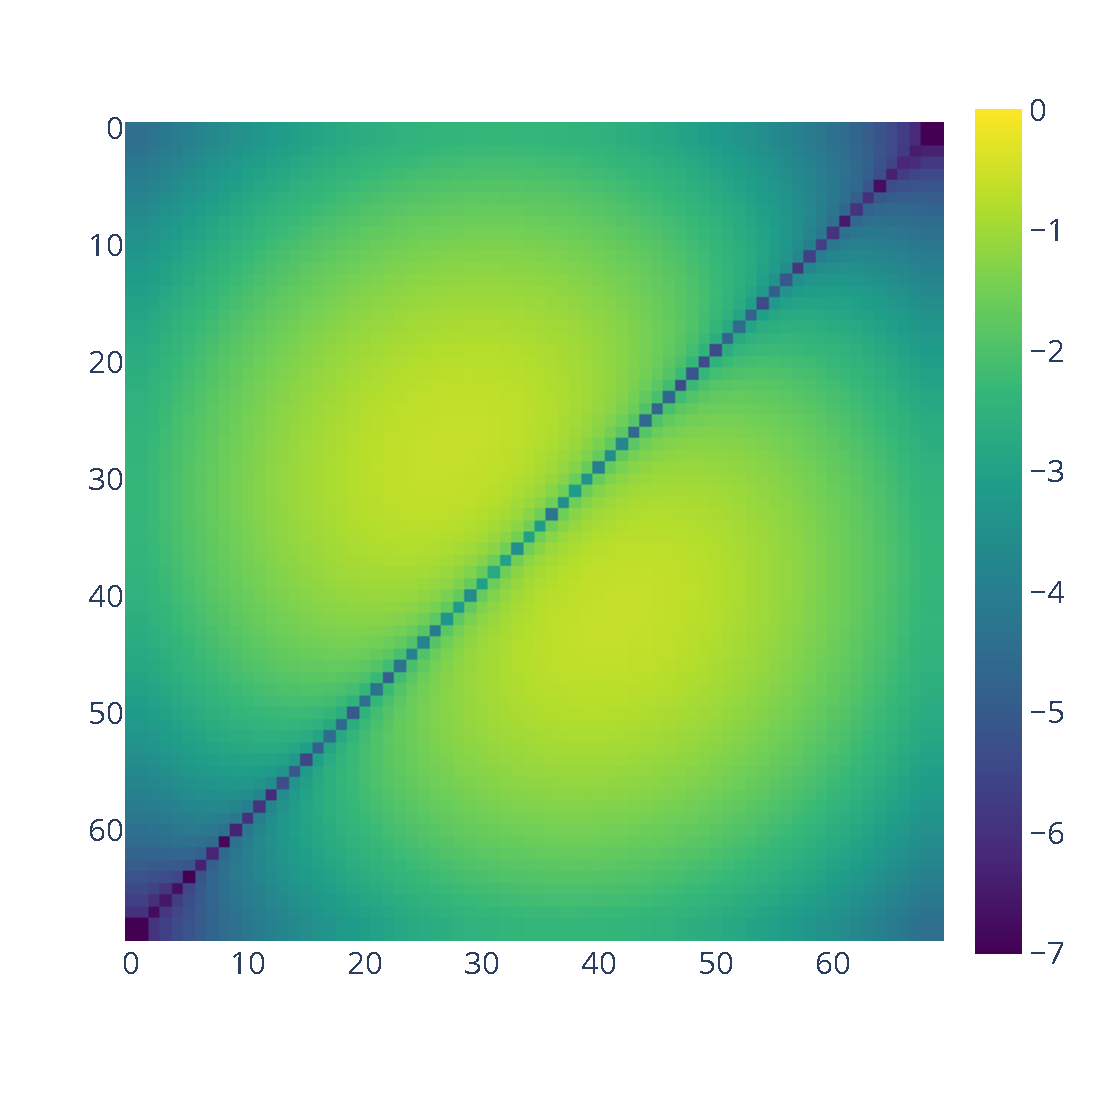
\includegraphics[width=\linewidth]{figure/spline_2d/bisplev_mean_log.pdf}
        \caption{Absolute mean value (log)}
        \label{fig:bisplev_mean_log}
    \end{subfigure}
    \begin{subfigure}{.3\linewidth}
        \centering
        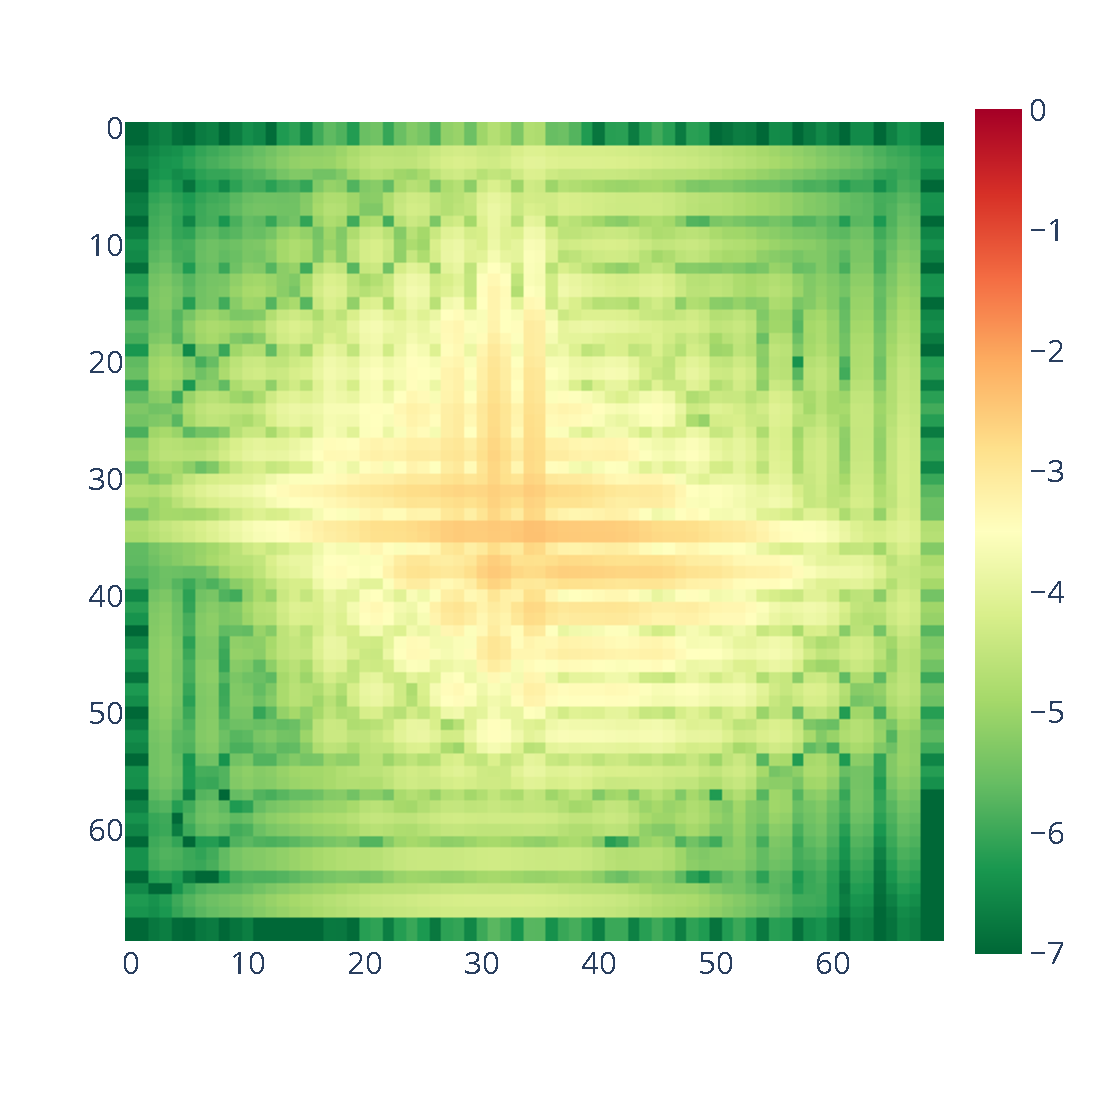
\includegraphics[width=\linewidth]{figure/spline_2d/bisplev_std_log.pdf}
        \caption{Standard deviation (log)}
        \label{fig:bisplev_std_log}
    \end{subfigure}
    \caption{2D Spline interpolation results. Figure~\ref{fig:bisplev_mean}
        shows the mean result of the 2D-spline interpolation.
        Figures~\ref{fig:bisplev_mean_log} and~\ref{fig:bisplev_std_log} show
        respectively in the logarithmic scale the absolute mean value and the
        standard deviation of the 5 samples run within RR mode. 
    }
    \label{fig:spline2d_rr}
\end{figure*}

\subsection{\pytracer allows visualizing numerical stability at a fine-grained level}


\add{We illustrate on two examples how PyTracer is effective for analyzing
    numerical stability in complex codes at a fine-grained level: Face recognition and Bayesian Ridge Regression.}
The face recognition example uses eigenfaces (eigenvectors) and Support Vector
Machines (SVMs) to classify faces from the Labeled Faces in the Wild dataset.
This example uses a Principal Component Analysis (PCA) to extract the eigenfaces
and then trains an SVM classifier to predict the label associated with a face.
\add{When executing in PyTracer, this example crashed because the Singular Value Decomposition (SVD) did not converge.}
This example is the only one to raise an error due to the
non-convergence of the SVD performed in the PCA.
The PCA uses the Randomized SVD~\cite{halko2011finding} method
that first computes a low-rank approximation of the input matrix using a
stochastic algorithm and then uses this approximation as input for the SVD. 
\add{When walking through the code with PyTracer, we see that}
the \texttt{randomized\_svd} scikit-learn function uses the Divide \& Conquer SVD
method \texttt{gesdd}. The LAPACK library has two main methods for computing the SVD:
\texttt{gesdd} and \texttt{gesvd}. The former uses a Divide \& Conquer approach,
while the latter uses a QR decomposition. While both methods are expected to
have the same accuracy~\cite{nakatsukasa2013stable}, the Divide \& Conquer
does not converge with MCA.

Replacing \texttt{gesdd} for \texttt{gesvd} solved the SVD convergence issue.
\pytracer allows to quickly visualize the new precision of the result.
Figure~\ref{fig:face_recognition_svd} shows the precision of the eigenvalues
computed displayed in decreasing order with \texttt{gesvd} \add{in single precision}, 
which varies between 15 and 20
significant bits out of the 24 available in single precision. The classifier
metrics (precision, recall, F1-score, and support) are identical to the IEEE
execution for all MCA samples. \add{We can note that even with the \texttt{gesvd} method,
    the precision of the singular values and eigenvectors is not uniform. 
    Indeed, we can see that the precision of the lowest singular values and eigenvectors decreases 
    until reaching 0 significant bits.}

The second example compares a Bayesian Ridge Regression (BRR) to the Ordinary
Least Squares (OLS) estimator on a synthetic dataset and for one-dimensional
regression using polynomial feature expansion. Although the example does not
raise a runtime error, the regression coefficients computed from the fitting are
non-significant. \pytracer traces reveal that the SVD solver used is once again the root
cause for this error. \add{Indeed, the BayesianRidge model first computes an SVD
    before iteratively updating the coefficients until reaching the convergence
    criterion. However, PyTracer shows an issue in the singular values computed.}
\add{We can see in Figure}~\ref{fig:BRR_svd} \add{that the last singular values is
    \texttt{NaN} due to numerical errors in the SVD, although the remaining
    singular values exhibit high numerical precision (between 44 and 50 bits).
    Surprinsingly, this \texttt{NaN} value does not raise an exception and is silently
    propagated. Indeed, the stopping criterion is never verified and the 
    optimization stops after reaching the maximal number of iterations.
    Figure}~\ref{fig:BRR_svd_fixed} \add{shows that uses
    the \texttt{gesvd} instead of the \texttt{gesdd} method removes the \texttt{NaN} value
    although the last singular values stills have a low precision (below 0).
    Following Equation}~\ref{eq:sig-digits}, \add{a number of significant digits below 0 means that the
    variability ($\sigma$) is higher than the average value ($\mu$)}.


\add{Similarly, for OLS, PyTracer tracers show that the
    regression coefficients fitted are \texttt{NaN} values. By looking at the callgraph, we can
    see that the scipy calls the \texttt{lstsq} method from the
    \texttt{scipy.linalg} package which uses the \texttt{gesdd} LAPACK function.
    Figure}~\ref{fig:OLS_svd} \add{shows that one singular value is a \texttt{NaN} value,
    which corrupted the calculation of the coefficients. When using the \texttt{gesvd} method, 
    the \texttt{NaN} value disapears 
    (Fig.}~\ref{fig:OLS_svd_fixed}\add{), resulting in a precision of
    42 bits in average in the coefficients. We can see that having
    access to all the values computed by the application with PyTracer allows
    the user to efficiently identify numerical issues.}

In conclusion, \pytracer and the MCA model were helpful to detect the
instability of the \texttt{gesdd} method mentioned in several GitHub issues,
including the LAPACK repository. Furthermore, it is worth mentioning that a Pull
Request has recently been submitted to let the user select the SVD method and
avoid this kind of issue. Thus, \pytracer can detect instabilities that affect
fundamental scientific computing components such as the LAPACK library. \add{The
    unified view of all traces allows the user to quickly navigate through the
    numerical precision of different variables.}
% The Pytracer findings can therefore be extended to many application domains. %
% \tristan{conclusion needs to be discussed. Note to self: generaliser un peu la
% conclusion: pytracer permet de se rendre compte de problemes de stabilite dont
% plusieurs librairies sont dependantes.}



\begin{figure*}
    \centering
    \begin{subfigure}{0.3\linewidth}
        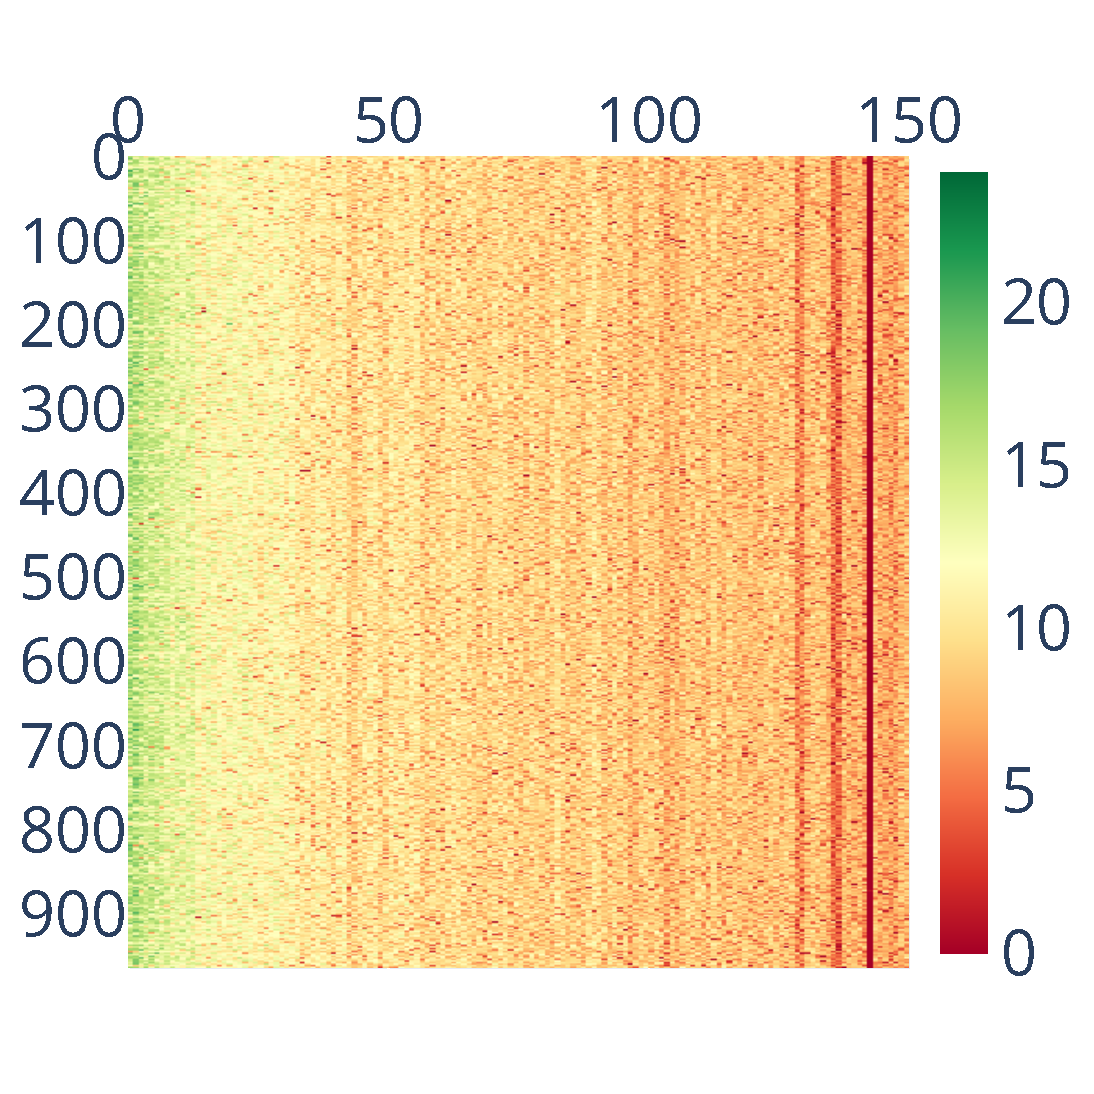
\includegraphics[width=\linewidth]{figure/face_recognition/randomized_svd_ret_U_sig.pdf}
        \caption{Left matrix $U$ of the SVD decomposition}
        \label{fig:randomized_svd_U}
    \end{subfigure}
    \begin{subfigure}{0.3\linewidth}
        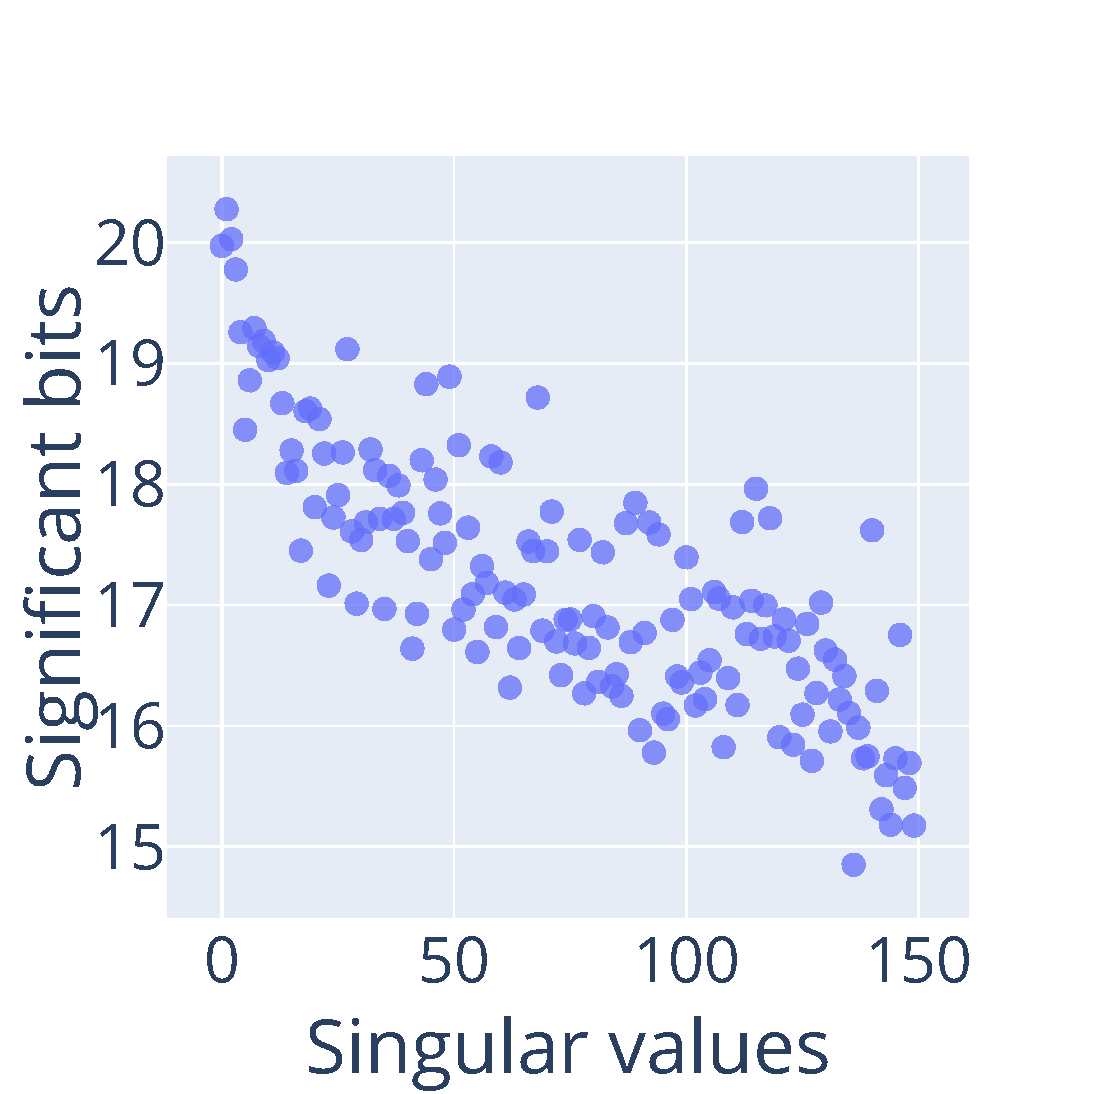
\includegraphics[width=\linewidth]{figure/face_recognition/svd_ret_S_sig.pdf}
        \caption{Singular values $\Sigma$ of the SVD decomposition}
        \label{fig:randomized_svd_S}
    \end{subfigure}
    \begin{subfigure}{0.3\linewidth}
        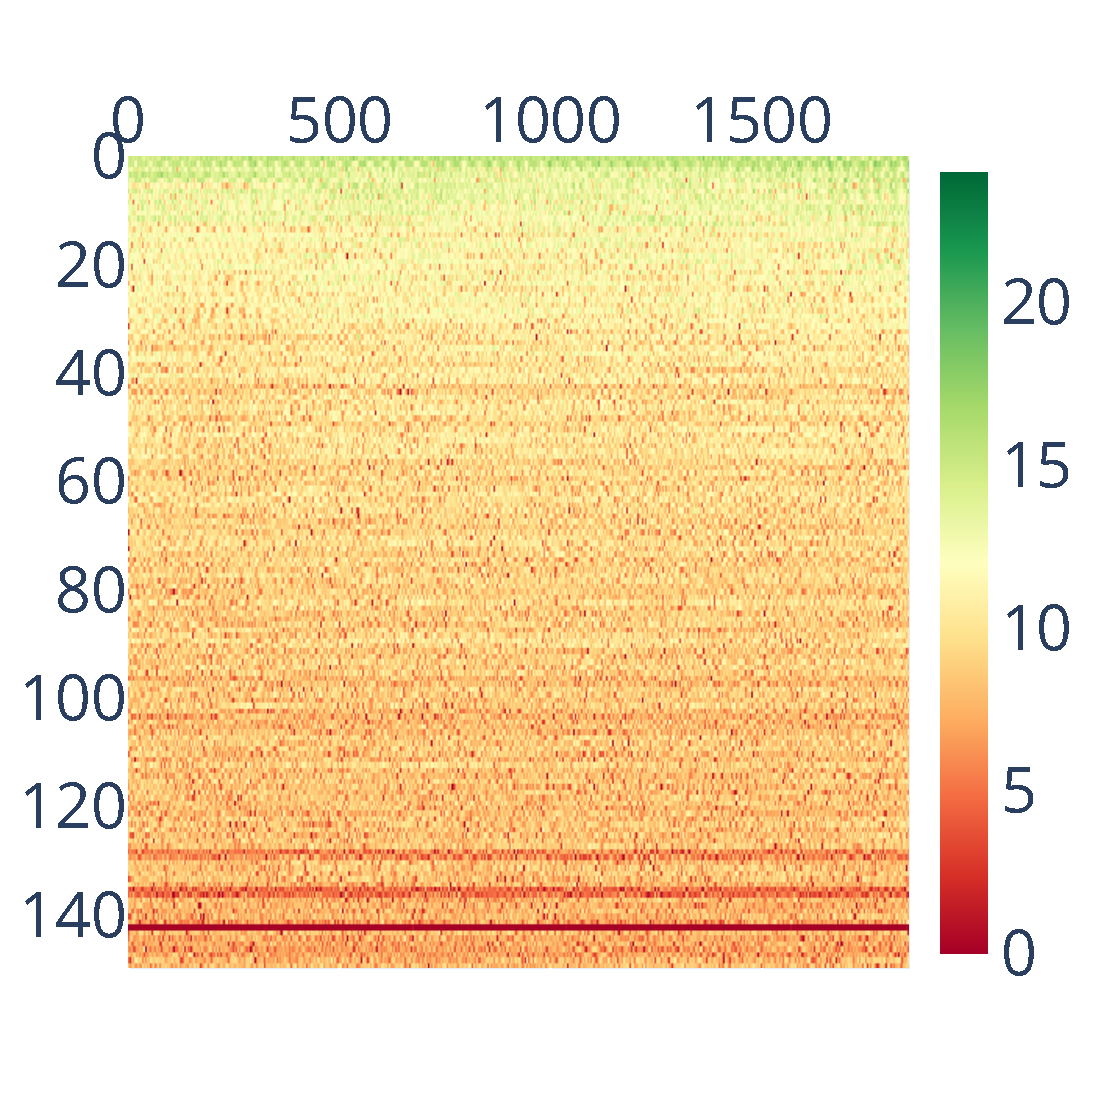
\includegraphics[width=\linewidth]{figure/face_recognition/randomized_svd_ret_V_sig.pdf}
        \caption{Right matrix $V$ of the SVD decomposition}
        \label{fig:randomized_svd_V}
    \end{subfigure}
    \caption{Precision of the \texttt{randomized\_svd} function in the
        \texttt{face\_recognition} example using the \texttt{gesvd} SVD method
        and RR. Figures~\ref{fig:randomized_svd_U},~\ref{fig:randomized_svd_S},
        and~\ref{fig:randomized_svd_V} show respectively the values $U$,
        $\Sigma$ and $V$. Numerical precision is lower for smaller singular
        values and this loss of precision translates to singular vectors. It
        would be interesting to investigate the use of numerical precision for
        dimensionality reduction. }
    \label{fig:face_recognition_svd}
\end{figure*}

\begin{figure}
    \centering
    \begin{subfigure}{0.49\linewidth}
        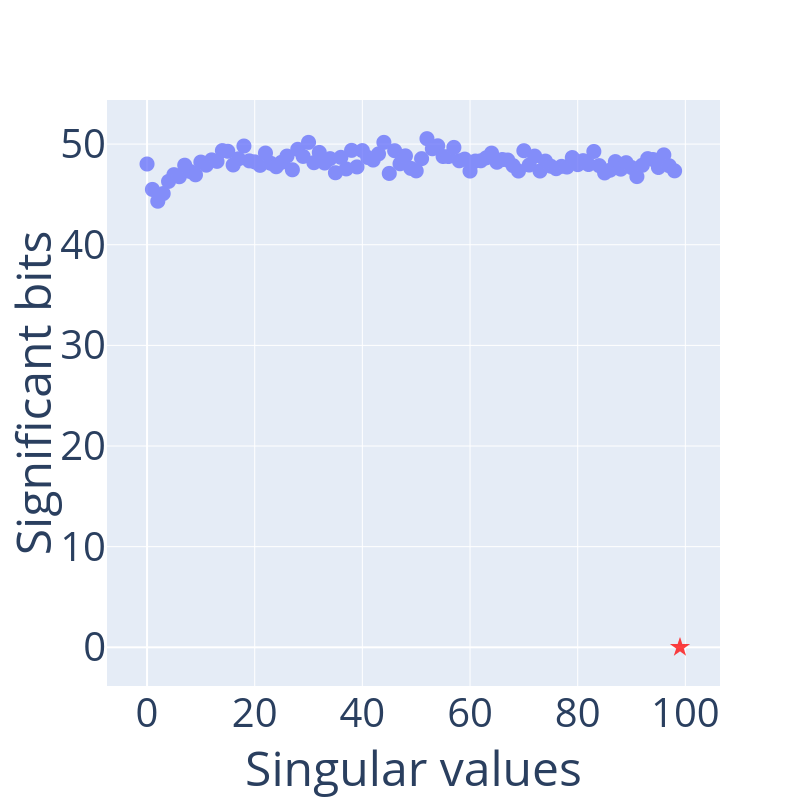
\includegraphics[width=\linewidth]{figure/BRR_singular_values.png}
        \caption{BRR (\texttt{gesdd})}
        \label{fig:BRR_svd}
    \end{subfigure}
    \begin{subfigure}{0.49\linewidth}
        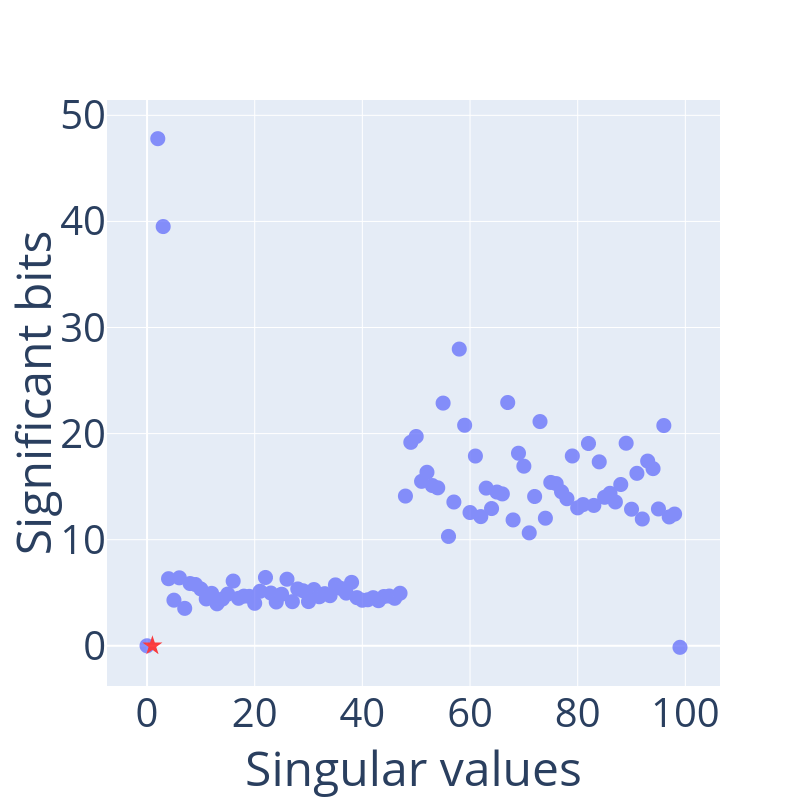
\includegraphics[width=\linewidth]{figure/OLS_singular_values.png}
        \caption{OLS (\texttt{gesdd})}
        \label{fig:OLS_svd}
    \end{subfigure}
    \begin{subfigure}{0.49\linewidth}
        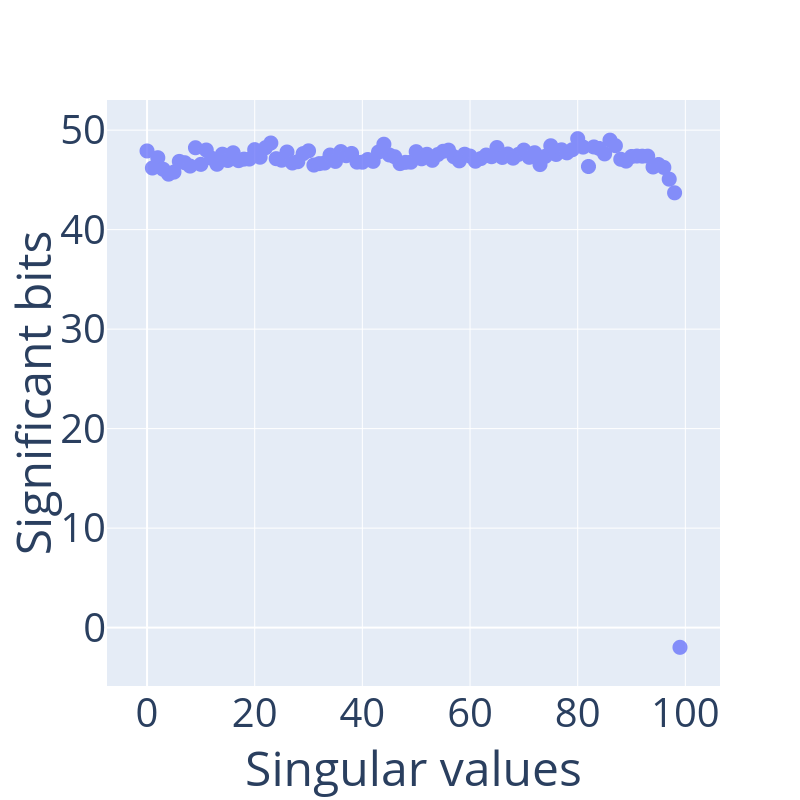
\includegraphics[width=\linewidth]{figure/BRR_singular_values_fixed.png}
        \caption{BRR (\texttt{gesvd})}
        \label{fig:BRR_svd_fixed}
    \end{subfigure}
    \begin{subfigure}{0.49\linewidth}
        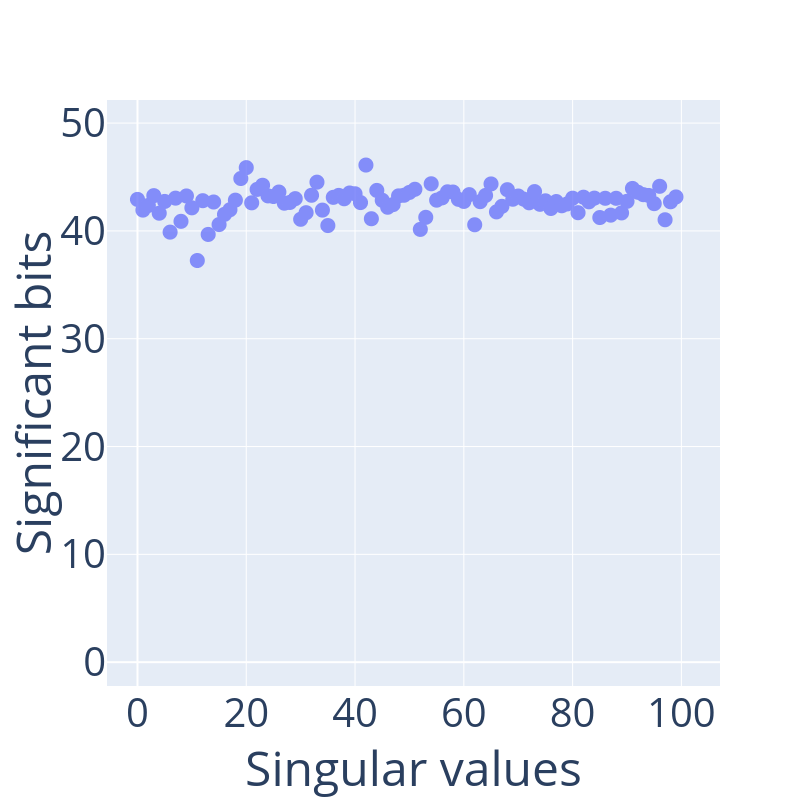
\includegraphics[width=\linewidth]{figure/OLS_singular_values_fixed.png}
        \caption{OLS (\texttt{gesvd})}
        \label{fig:OLS_svd_fixed}
    \end{subfigure}
    \caption{\add{Numerical precision of the singular values of the SVD from the
            Bayesian Ridge model fitting (left) and from the Ordinary Least Square model
            fitting (right) in the Bayesian Ridge Regression example. Red stars
            represent \texttt{NaN} values. 
            Switching from Divide \& Conquer (\texttt{gesdd}) to QR (\texttt{gesvd}) factorization improves numerical precision.
            PyTracer helps visualizing improvements.}}
\end{figure}

\subsection{\pytracer instrumentation limitations}

\add{
    The limitations of the PyTracer's instrumentation have little impact in practice
    since we have encountered few classes having non-writeable attributes in practice.
    Moreover, those classes are generally used in higher-level classes written in
    pure Python. For instance, the SGD class that implements the Stochastic Gradient
    Descent in scikit-learn takes a loss function as a parameter. Loss functions are
    implemented in Cython in scikit-learn and Pytracer is not able to instrument
    them. However, Pytracer can dump the instance of LossFunction if they are used
    by the SGD class as arguments, which is a frequently observed pattern in
    Scikit-learn for instance. So one still has an estimation of variability for the
    attributes of the class. Finally, one can use Veritracer to trace the methods of
    those Cython classes for an in-depth analysis since it is the C language
    underhood. We have encountered few iterators and none of them involved floating
    point values so we were able to safely ignore them. 
}

\subsection{Overhead remains tractable and evolves linearly with the trace size}

\pytracer's tracing overhead consists of (1) module instrumentation time
(initialization overhead) and (2) data write time during the execution (runtime
overhead). The initialization overhead is proportional to the number of
functions and classes traced. For example, we measured an average initialization
time of 8 seconds during our experiments with  NumPy, SciPy, and Scikit-learn.
This overhead can be reduced by excluding intensively used functions such as
\texttt{numpy.array} from the instrumentation.
Figure~\ref{fig:performance_tracing} summarizes \pytracer's tracing overhead for
SciPy and scikit-learn examples. \textit{Slowdown} represents the slowdown of
\pytracer without fuzzy measured as the ratio between the actual execution time
(without \pytracer) and the execution time using \pytracer. The \textit{Slowdown
    RR} \remove{and \textit{Slowdown MCA}} shows the slowdown within the Fuzzy environment.
Without Fuzzy, \pytracer introduces an average slowdown of $17\times$ for
the examples running less than 8 seconds because \pytracer spends most of its
time in the initialization step. Since this step is a constant factor of the
number of functions instrumented, we also measured the instrumentation cost
itself (\textit{Slowdown (Instrumentation)}) calculated by subtracting the
initialization time to \textit{Slowdown}. We then obtain an average slowdown of
$3.5\times$. Finally, the \remove{Fuzzy instrumentation} \add{using MCA
    operations (through Fuzzy) instead of the native ones} increases the average
slowdown to $37\times$ for RR\remove{and $43\times$ for Full MCA}.

% \pytracer's tracing overhead consists of (1) module instrumentation time
% (initialization overhead), and (2) data write time during the execution
% (runtime overhead). The initialization overhead is proportional to the number
% of functions and classes traced. However, the initialization overhead is
% amortized \tristan{what do you mean by amortized? I don't get this sentence}
% when traced applications are above 8 seconds,  proportional to the number of
% functions and classes traced. Figure~\ref{fig:performance_tracing} summaries
% \pytracer's tracing overhead for SciPy and scikit-learn examples. We can see
% that \pytracer introduces a slowdown of reduced toif we subtract the
% initialization step \tristan{not sure where to get these numbers from the
% table, to be clarified. Are these average values? Why are there two values?}.
% Fuzzy instrumentation increases the slowdown to for RR and   for Full MCA.
% \tristan{Figure 13 is not referred in the text. Choose between the figure and
% the table, no need to put both.}

\begin{figure}
    \centering
    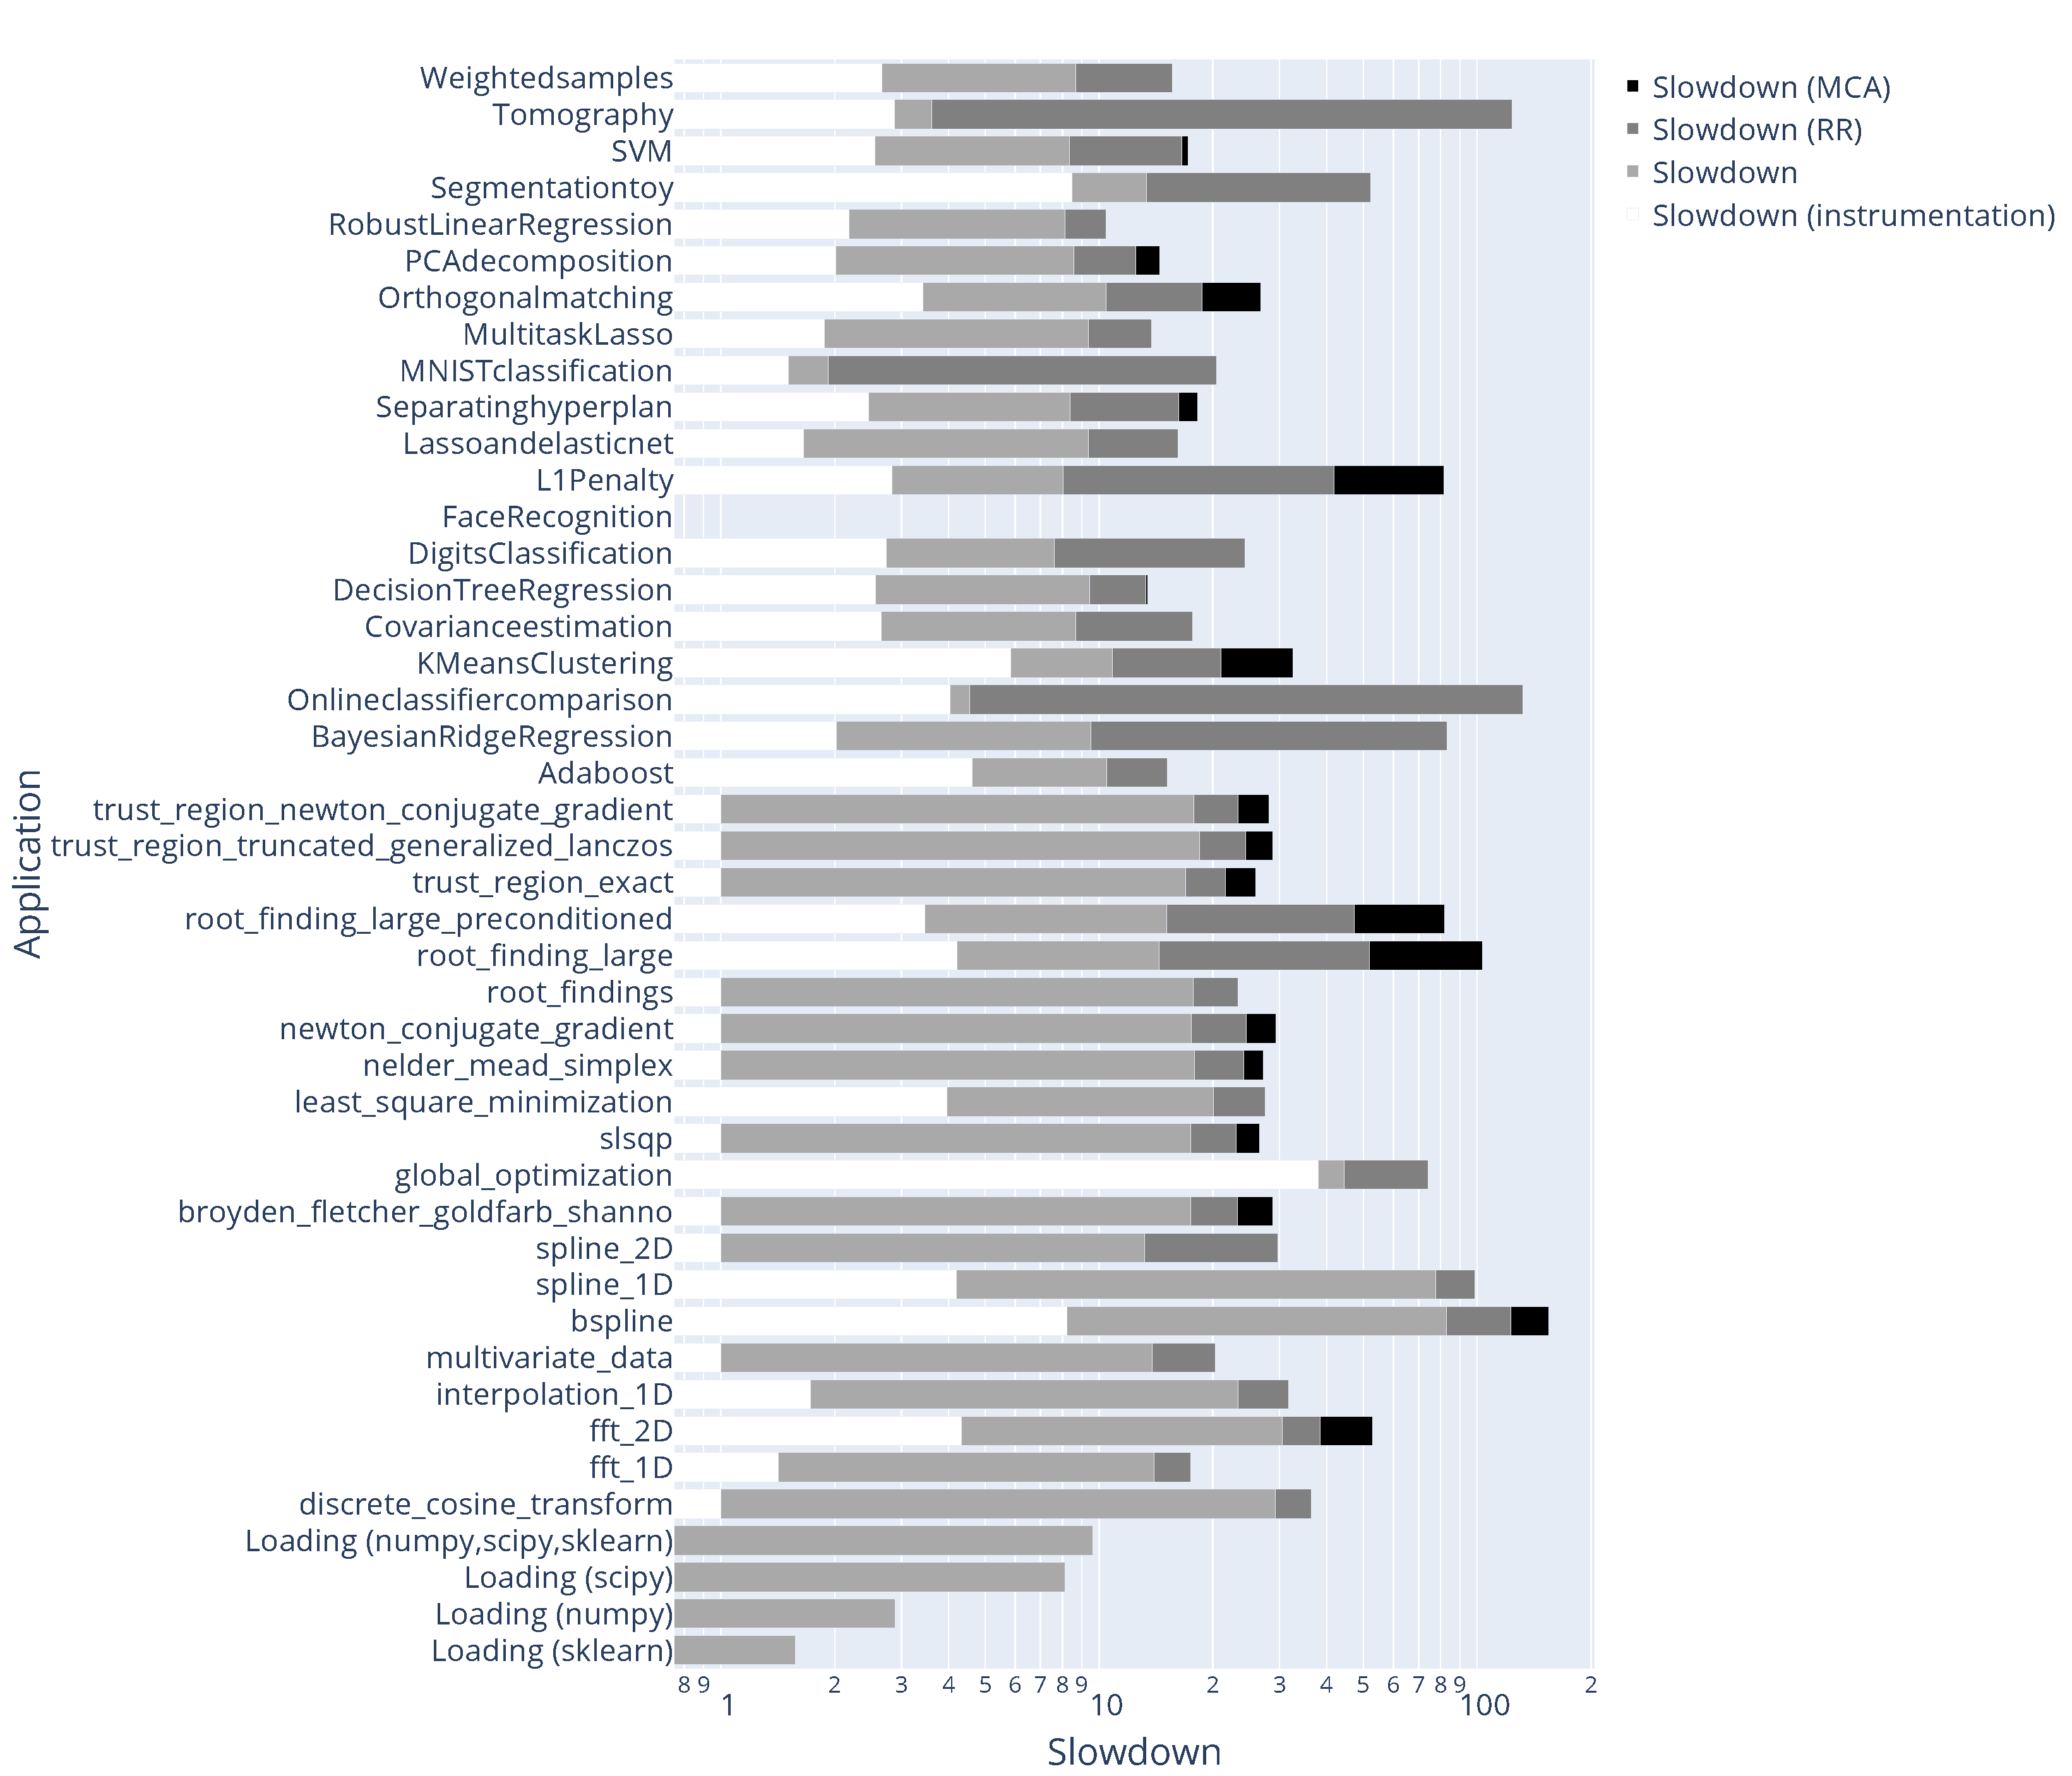
\includegraphics[width=\linewidth]{figure/performance.pdf}
    \caption{
        \pytracer tracing overheads. \textit{Slowdown} represents the slowdown
        of \pytracer without Fuzzy measured as the ratio between the actual
        execution time (without \pytracer) and the execution time using
        \pytracer. \textit{Slowdown (Instrumentation)} show the actual
        instrumentation cost computed by subtracting the initialization step.
        The \textit{Slowdown (RR)} \remove{and \textit{Slowdown (MCA)} are} \add{is} the slowdown
        of \pytracer using the Fuzzy environment with \add{the} RR \remove{and Full MCA} mode\remove{s}. The
        \remove{first} \add{last} four examples measure the initialization
        steps depending on the modules instrumented. 
        % \tristan{there's too much text in this caption, move some of it to the text, the caption should just explain the difference between the 4 slowdowns. From the text I'm not sure what is the difference between slowdown and slowdown(RR)/slowdown(MCA).}
    }
    \label{fig:performance_tracing}
\end{figure}

% \begin{figure}
%     \centering
%     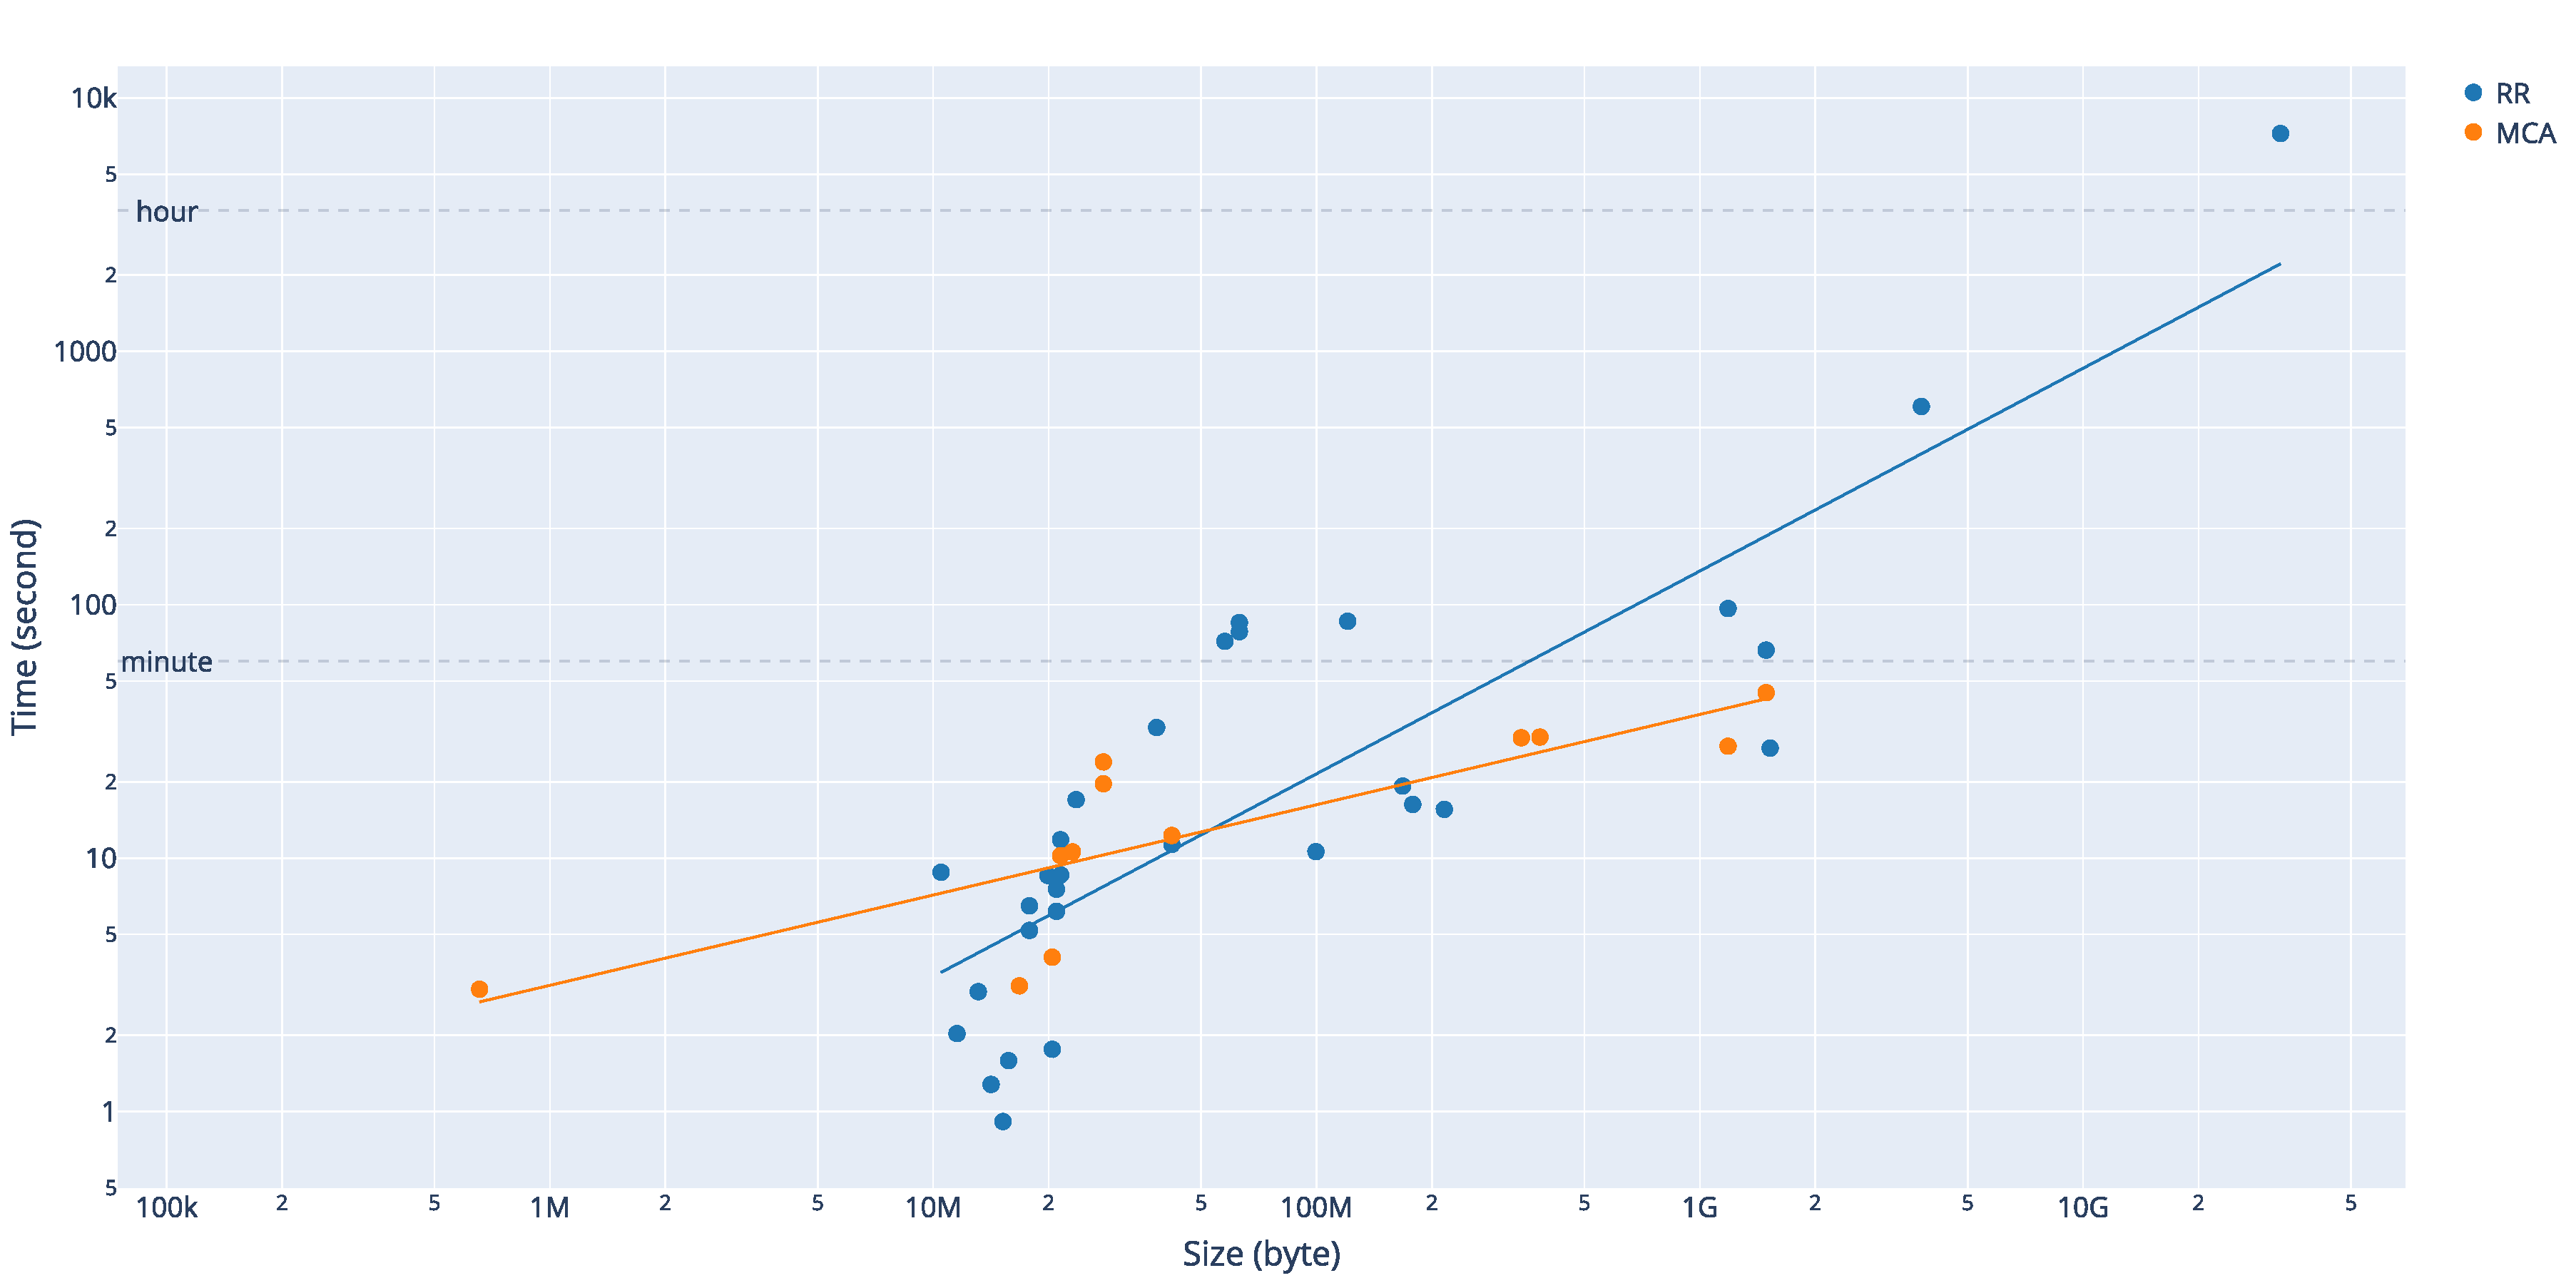
\includegraphics[width=\linewidth]{figure/parsing_time.pdf}
%     \caption{\pytracer time to aggregate traces.}
%     \label{fig:performance_parsing_time}
% \end{figure}

% \begin{figure}
%     \centering
%     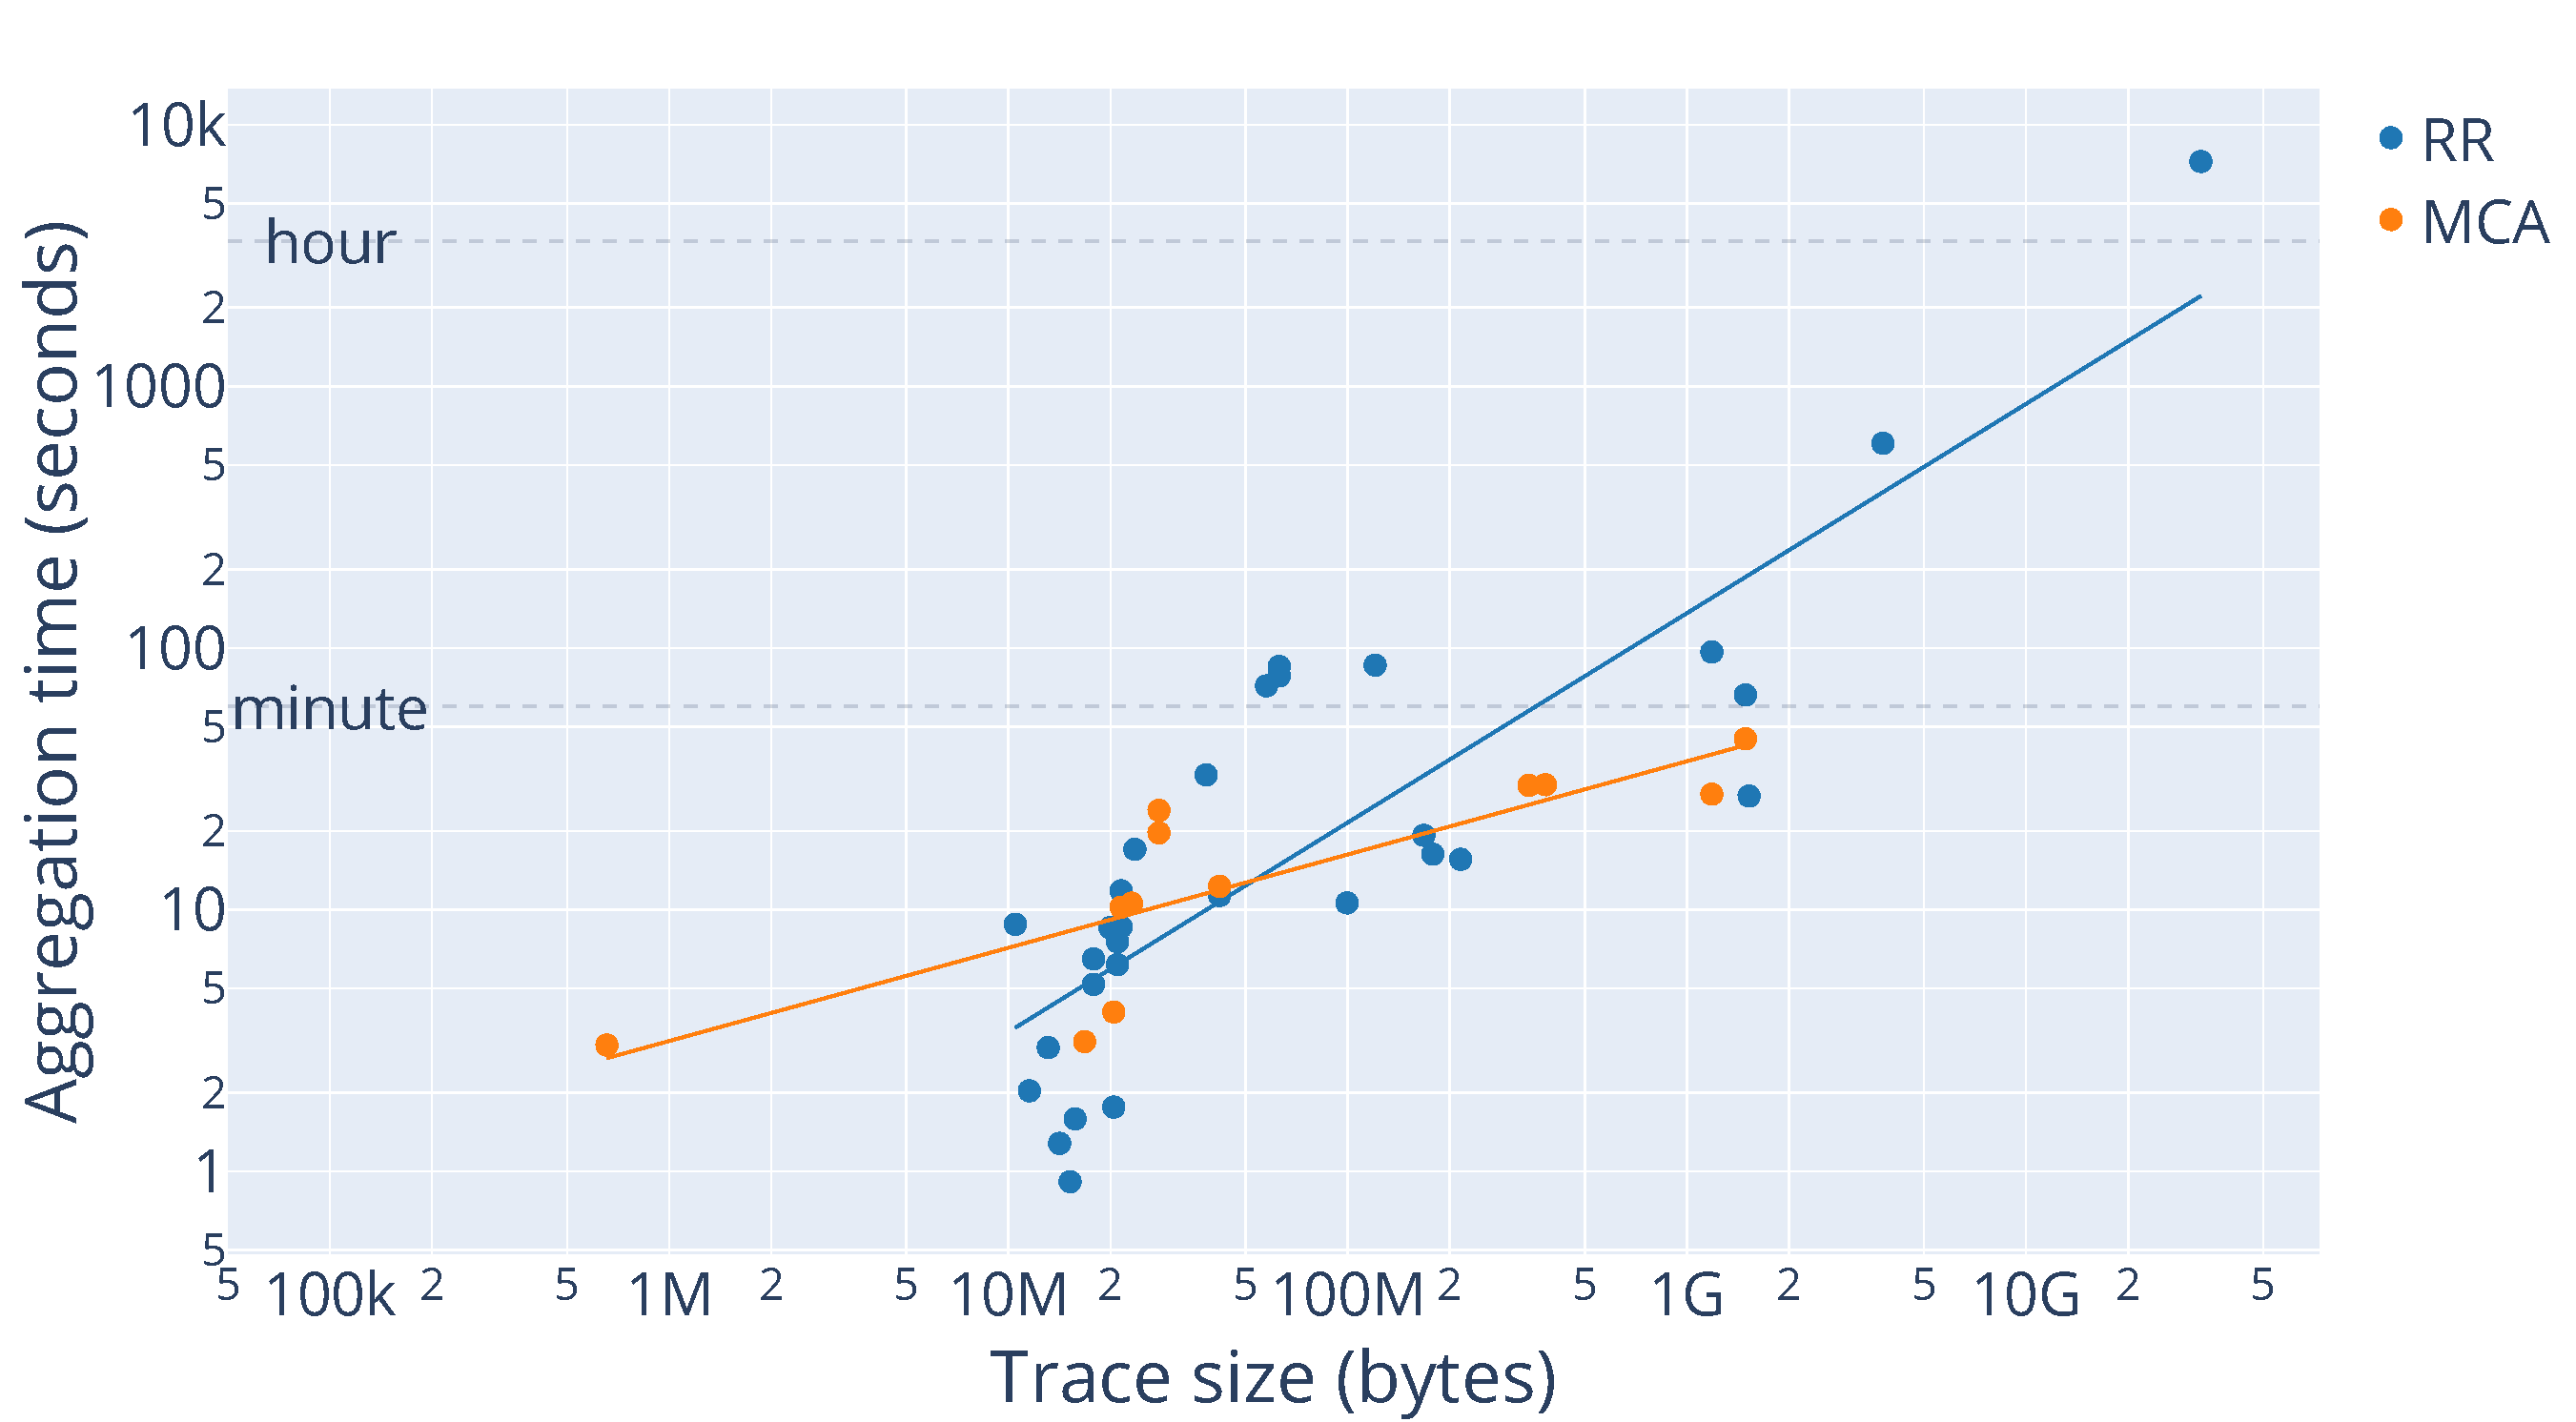
\includegraphics[width=\linewidth]{figure/parsing.pdf}
%     \caption{\pytracer trace and aggregation files size.
%     The figure presents the size measured for the trace and the aggregation size files.}
%     \label{fig:performance_parsing_size}
% \end{figure}

\begin{figure}
    \centering
    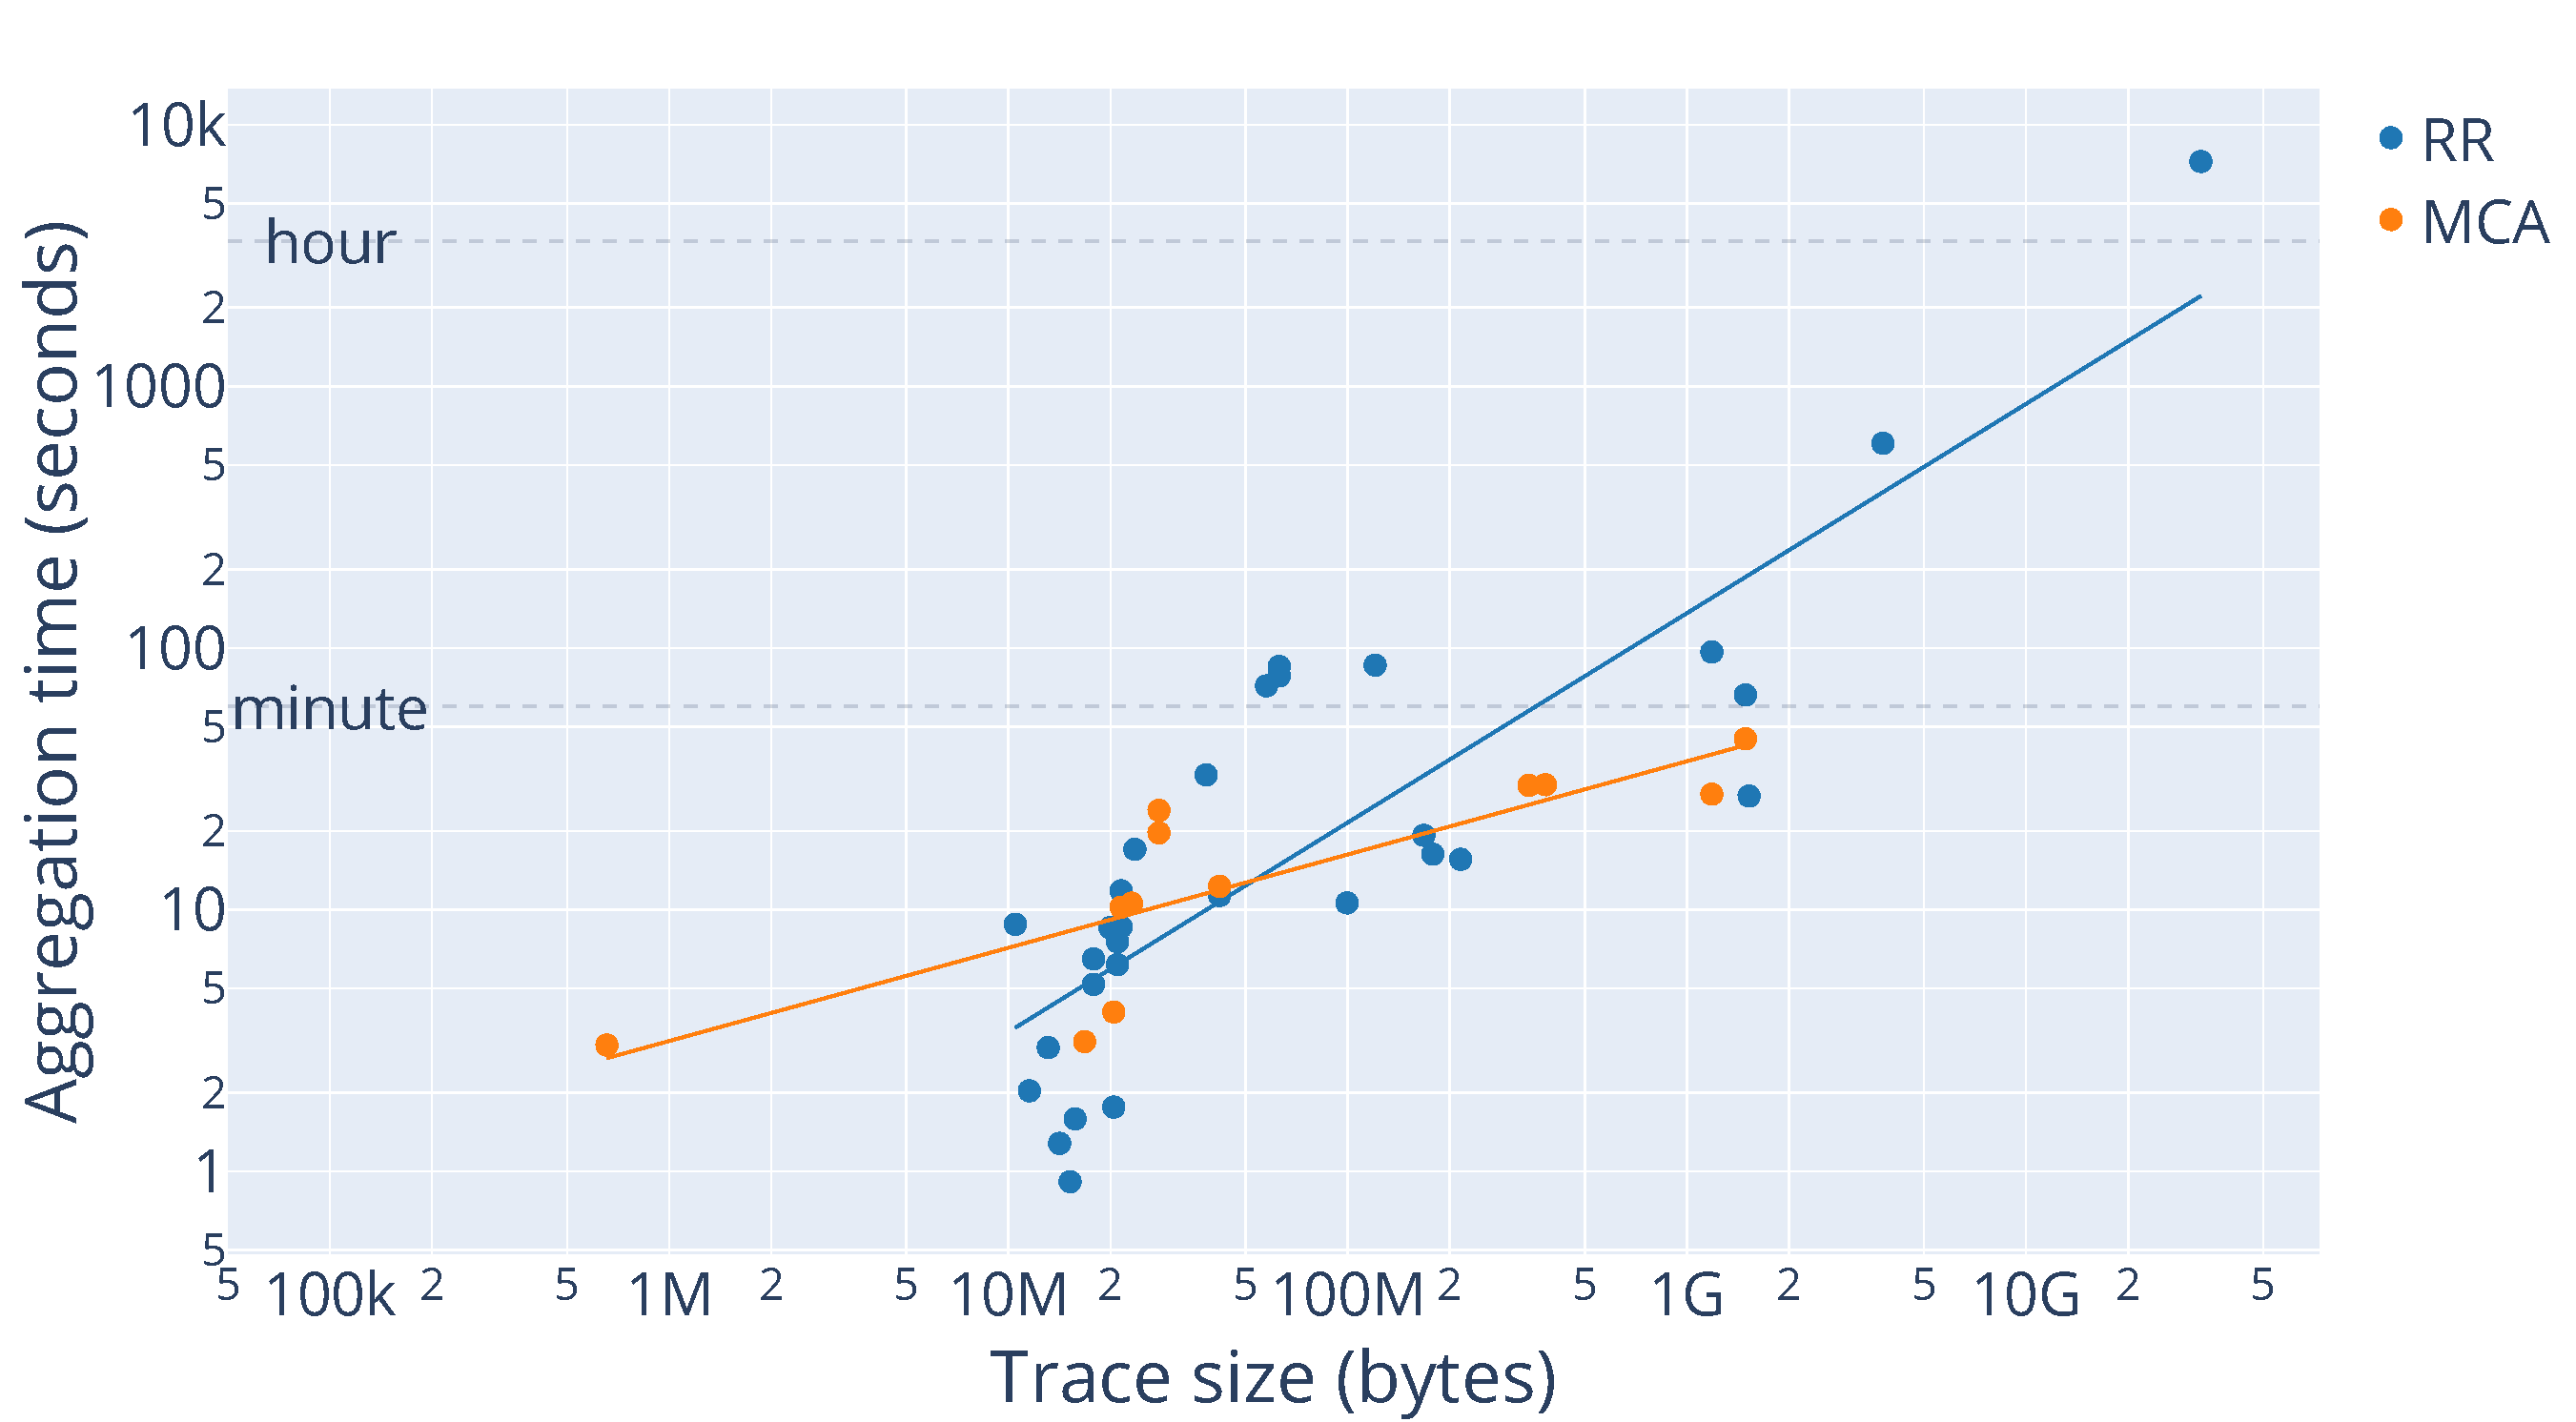
\includegraphics[width=\linewidth]{figure/performance_parsing.pdf}
    \caption{\pytracer aggregation performance.
        % \tristan{change xlabel to "Trace size (bytes) and ylabel to "Aggregation time (seconds)}
    }
    \label{fig:performance_parsing}
\end{figure}

% \begin{table}
% \centering
% \begin{subfigure}[t]{.75\linewidth}
%     \centering
%     \begin{tabular}{|l|c|c|c|c|}
%     \hline 
%     Application & Original & Pytracer only & RR & MCA \\
%     \hline 
%     Loading & 0.456 & 8.152 & - & - \\
%     \hline
%     discrete\_cosine\_transform & 0.280 & 8.176 & 10.203 & - \\ 
%     fft\_1D & 0.650 & 9.075 & 11.345 & - \\
%     fft\_2D & 0.311 & 9.500 & 11.929  & 16.433   \\
%     \hline
%     interpolation\_1D & 0.377 & 8.803  & 11.954  & -   \\
%     multivariate\_data &0.626 & 8.648 &  12.711  & - \\
%     bspline & 0.109  & 9.050 & 13.396  & 16.830   \\
%     spline\_1D & 0.111 & 8.618 & 10.960   & - \\
%     spline\_2D & 0.655 & 8.649 & 19.424  & - \\
%     \hline
%     broyden\_fletcher\_goldfarb\_shanno &0.475 & 8.292 & 11.033 & 13.685 \\
%     global\_optimization &1.257 & 55.916  & 93.322  & - \\
%     slsqp & 0.469 & 8.192 & 10.795 & 12.439  \\
%     least\_square\_minimization & 0.505 & 10.151  & 13.888 & -  \\
%     nelder\_mead\_simplex & 0.471 & 8.418  & 11.382  & 12.792  \\
%     newton\_conjugate\_gradient & 0.487 & 8.548  & 11.956  & 14.281 \\
%     root\_findings & 0.462 & 8.198  & 10.787   & - \\
%     root\_finding\_large & 0.801 & 11.525 & 41.493   &  82.701  \\
%     root\_finding\_large\_preconditioned & 0.702 & 10.580 & 33.199   & 57.579  \\
%     trust\_region\_exact & 0.482 & 8.170 & 10.400  & 12.524 \\
%     trust\_region\_truncated\_generalized\_lanczos & 0.459 & 8.457 & 11.216 & 13.245  \\
%     trust\_region\_newton\_conjugate\_gradient & 0.479 & 8.538 & 11.179 & 13.488 \\
%     \hline
%     Adaboost &1.388 &14.553 &  20.999 & - \\
%     Bayesian Ridge Regression & 1.086 & 10.344 & 90.299 & -  \\
%     Online classifier comparison & 15.964 & 72.691 & 2104.114 & -  \\
%     K-Means Clustering & 1.621 & 17.614  & 34.005 & 52.902   \\
%     Covariance estimation & 1.357 & 11.755 & 23.964  & -   \\
%     Decision Tree Regression & 1.185 & 11.194 & 15.760 & 15.918  \\
%     Digits Classification & 1.672 & 12.725 & 40.634 & - \\
%     Face Recognition & 32.159  & 74.356 & - & - \\
%     L1 Penalty & 1.568 & 12.591 & 65.547 & 128.220 \\
%     Lasso and elastic net & 1.057 & 9.903 & 17.078 & -  \\
%     Separating hyperplan & 1.376 & 11.532  & 22.333 & 25.036 \\
%     MNIST classification & 19.650 & 37.838 & 402.389  & - \\
%     Multitask Lasso & 1.090 &10.196 & 15.025  & - \\
%     Orthogonal matching & 1.161 & 12.129 & 21.779   & 31.135 \\
%     PCA decomposition & 1.239 & 10.642 & 15.520 & 17.952    \\
%     Robust Linear Regression & 1.370 & 11.144  & 14.280  & - \\
%     Segmentation toy &1.679 & 22.385 & 87.811  & - \\
%     SVM & 1.403 & 11.737 & 23.203 & 24.126   \\
%     Tomography & 11.108 & 40.177  & 1376.134 & -  \\
%     Weighted samples & 1.358 & 11.768 & 21.255 & 20.541   \\
%     \hline
%     \end{tabular}
% \end{subfigure}
%     \caption{\pytracer tracing overhead in seconds. \tristan{what is the unit in this table?}}
%     \label{tab:pytracer_overhead}
% \end{table}


% \begin{table}[]
%     \centering
%     \begin{tabular}{c|c|c|c|c}
%          Pytracer & Verificarlo Instrumentation & Backend & Time (hours:minutes:seconds) & Overhead \\
%          \hline 
%          No & No & - & 00:30:51 & 1 \\
%          No & Yes & IEEE & 01:32:56 & 3 \\
%          No & Yes & RR & 16:52:08 & 32 \\
%          Yes & No & - & 03:11:07 & 6  \\
%          Yes & Yes & IEEE & 11:14:33 & 22 \\
%          Yes & Yes & RR & 25:05:54 & 48 \\
%     \end{tabular}
%     \caption{Overheads of \pytracer on PyAFQ experiment with and without fuzzy.}
%     \label{tab:pytracer_overhead}
% \end{table}

% \begin{table}[]
%     \centering
%     \begin{tabular}{c|c|c|c|c}
%          Pytracer & Verificarlo Instrumentation & Backend & Time (hours:minutes:seconds) & Overhead \\
%          \hline 
%          No & No & - & 15 & 1 \\
%          No & Yes & IEEE & 49 & 3 \\
%          No & Yes & RR &  & 441 & 29 \\
%          Yes & No & - & 03:11:07 & 6  \\
%          Yes & Yes & IEEE & 11:14:33 & 22 \\
%          Yes & Yes & RR & 25:05:54 & 48 \\
%     \end{tabular}
%     \caption{Caption}
%     \label{tab:pytracer_overhead}
% \end{table}

Figure~\ref{fig:performance_parsing} shows the postprocessing time and trace
sizes produced by \pytracer. The linear correlation between the log of the size
and the log of the time shows a significant correlation (p-value $\leq 10^{-8}$
\remove{for RR and p-value $\leq 10^{-3}$ for MCA}).
% \tristan{Mention linear correlation with p-value here.}

In conclusion, while \pytracer's overhead is substantial, it remains tractable
for real-life examples.

\section{Discussion}

% Numpy   2509 (2403 not tests) (1848) functions, 1196 (1154) (817) classes (pure Python)
% Scipy   4031 (2187) (506) functions, 1532 (472) (109) classes (pure Python)
% Sklearn 4807 (1010) (81) functions, 546 (417) (41) classes (pure Python)

% \pytracer is a tool for visualizing the numerical quality of function inputs
% and outputs along the execution of a Python program. It generates numerical
% traces and post-processes them to measure numerical discrepancies between
% executions. \pytracer does not require any particular noise model to estimate
% uncertainties. We tested it with MCA through the fuzzy ecosystem on two
% broadly used Python libraries.

Through our analysis of SciPy and scikit-learn, we demonstrated \pytracer's
scalability, automaticity, and applicability to a wide range of Python programs.
The relatively low instrumentation overhead of 3.5$\times$ on average enables
the analysis of real-scale applications. \pytracer's instrumentation is fully
automatic and does not require manual intervention from the user. Furthermore,
\pytracer works with any Python libraries, with any data format supported by
pickle and any numerical noise model.

\pytracer is the first tool to enable a systematic numerical analysis of Python
codes. Existing tools focus on traditional languages of the HPC community, such
as C, C++, and FORTRAN. However, Python's high-level abstraction allows for
quick application implementations while maintaining high-performance thanks to
specialized libraries such as NumPy. Therefore, \pytracer meets the numerical
analysis needs of an ever-increasing number of applications.

\pytracer allows users to pinpoint the root causes of numerical instabilities by
working at the level of Python functions. Numerical stability evaluations are complex since
calculations are strongly interdependent. Function-level instrumentation limits
the size of the traces since only inputs and outputs of a function are dumped.
Moreover, it decreases instrumentation overhead and helps the user identify
instabilities quickly. Working at the function level is thus a suitable
compromise between analyses conducted at the floating-point operation level and
user debug prints. Indeed, operation-level analyses are costly and hard to
interpret as they overwhelm users with information. In contrast, looking at
intermediate results through print statements is lightweight but not reliable
since developers may not systematically instrument unstable functions. 

\add{\pytracer can be used with different types of numerical perturbations,
including random seeds, data noise, or stochastic arithmetic. The
use of Verificarlo to implement stochastic arithmetic through the Fuzzy
environment enables to study the impact of numerical perturbations
introduced in non-Python dependencies while preserving the high-level view
of Python variables and functions. For instance, the SciPy environment
wraps many computation kernels written in C, such as BLAS or LAPACK, which
have a considerable impact on the stability of applications using them.}

\add{
Enabling Monte-Carlo arithmetic in such non-Python dependencies requires
their recompilation with Verificarlo, which usually requires human
intervention. The Fuzzy environment provides pre-instrumented version of
NumPy, BLAS, LAPACK, GNU libmath, SciPy, and Scikit-learn, which, given the
prevalence of these libraries in scientific Python codes, should cover a
large ground of non-Python dependencies encountered in scientific Python programs.
}


Integrating \pytracer at the early stages of the development cycle would improve
the overall numerical quality of the developed code. \pytracer's automaticity
facilitates its usage and enables its integration in unit testing. For example,
\pytracer could be used in regression tests to ensure that updates do not
degrade the numerical quality of a calculation. 

\pytracer might also be useful for selecting hyperparameters, as is the case in
machine learning. Indeed, it is common for data scientists to explore a range of
hyperparameters and select the ones giving the best scores. With \pytracer, the
user has a practical way to quantify numerical quality and understand why
hyperparameters produce inconsistent results instead of tweaking hyperparameters
to make solvers converge. For instance, the Face Recognition example
(Figure~\ref{fig:face_recognition_svd}) shows how numerical precision could
inform the selection of the number of components in dimensionality reduction. 


\pytracer's visualization provides a global view of the code and interactions between
computations. In addition, the Plotly dashboard helps navigate through the code
easily, without the need for ad-hoc scripts to visualize data. The
dashboard can be extended to support other data formats to visualize. At this
stage, \pytracer currently supports n-dimensional NumPy arrays as well as native
Python data. 

\remove{
    As we showed in Section~\ref{sec:impact_mca_modes}, using Full MCA mode leads to
    runtime errors that have a considerable impact on the proper functioning of the
    execution, which is unfortunate since these errors do not reflect actual
    numerical errors but are related to perturbations that should not occur.
    Conversely, RR mode is far more conservative since it preserves exact operations
    and is easier to use even though it does not simulate all perturbations.
    Therefore, from our experiments, we recommend the use of RR over Full MCA. More
    research is required to address the issues encountered with Full MCA. 
}


Finally, the wide range of results precision observed in our experiments
suggests that such
analyses would benefit from being conducted systematically. We showed that
well-known scientific libraries are prone to numerical errors even though they
have been well tested for decades. The prevalence of these libraries in
scientific codes should thus impel users to integrate numerical analysis in
their development workflow in addition to testing their implementation.

\section{Related work}

Several tools have been developed to assess numerical quality, and can be
divided into static and dynamic approaches. Static approaches typically analyze
source code, while dynamic approaches trace floating-point computations
throughout executions. A detailed review of these approaches is presented
in~\cite{cherubin2020tools}. 
% \pytracer adopts the dynamic approach due to its scalability to large code
% bases. Dynamic approaches typically trace floating-point computations, detect
% instabilities in traces, and visualize summary statistics about instabilities.
% This section reviews existing approaches for each of these steps.
% \label{sec:soa} \paragraph{Numerical tracing techniques}
Numerous tools exists to trace floating-point computations for C, C++, or
FORTRAN programs due to the prevalence of these languages in High-Performance
Computing (HPC). The main tracing techniques are \textit{source-to-source},
\textit{compiler-based transformations}, and \textit{dynamic binary
    instrumentation}.

% \gkmod{}{Note: this paragraph just reads like a list with no real
% interpretation/commentary. I think it would be better to state the strengths
% of this technique, cite examples, and then state limitations/why it isn't the
% only technique used.}
The source-to-source technique requires a rewriting of the application to modify
floating-point types and provides a fine-grained control on the analyzed code.
CADNA~\cite{jezequel2008cadna} is a library for C, C++, and Fortran implementing
CESTAC~\cite{vignes1993stochastic} stochastic arithmetic.
Shaman~\cite{demeure_phd} is a C++ library that uses a first-order error model
to propagate numerical error. MCAlib~\cite{frechtling2015mcalib} is a C library
that implements the Monte Carlo Arithmetic (MCA)~\cite{parker1997monte} using
the MPFR~\cite{fousse2007mpfr} library. \add{ADAPT \mbox{~\cite{menon2018adapt}} uses
    Automatic Differentiation to compute a sensitivity profile for each variable in a
    program}. Finally, the work in~\cite{tang2016software} proposed a
source-to-source framework for executing targeted code in infinite and fixed
precision with and without stochastic arithmetic. The main drawback of the
source-to-source approach is its lacks of scalability since rewriting large
codes can be a tedious task.

% \gkmod{}{Note: similar to the above, this is just a list rather than a
% highlight of how the compiler-based approach can be more scalable than
% source-to-source because it requires less manual intervention into a codebase
% (e.g.), then have your list, and finally say why it is still limited/not a
% global fix to this problem.}

The compiler-based approach instruments floating-point expressions at compile
time and so allows the user to automatically instrument large codebases.
Verificarlo~\cite{verificarlo} is a compiler that supports different types of
arithmetic instrumentations, including MCA. The work in~\cite{bao2013fly}
modified the GNU Compiler Collection (GCC) to track local floating-point errors
across executions. pLiner~\cite{guo2020pliner} is a root-cause analyzer based on
the Clang compiler that detects floating-point operations responsible for result
variability using a source-to-source transformation at the Abstract Syntax Tree
(AST) level to rewrite parts of code with higher precision.
PFPSanitizer~\cite{chowdhary2020debugging,chowdhary2021parallel} \add{and
    NSan~\mbox{\cite{courbet2021nsan}} are compiler based approaches}
that use shadow execution to detect numerical issues using higher
precision.
FLiT~\cite{sawaya2017flit} is a framework to detect variability
induced by compilers and their optimizations. The work
in~\cite{wang2012development} proposes a numerical debugger based on
GDB~\cite{stallman1988debugging} for Discrete Stochastic Arithmetic (DSA) on
FPGA as an Eclipse plugging. Similarly, Cadtrace~\cite{jezequel2008cadna} and
Shaman propose a GDB-based tool to use the CADNA and Shaman libraries with GDB,
respectively. The main limitation of the compiler-based approach is that one
must have access to the source code.

Dynamic Binary Instrumentation (DBI) operates directly on executables, without
the need for recompilation or manual changes. Therefore, it is applicable to any
programming language. CraftHPC~\cite{lam2013dynamic} uses DBI to detect
catastrophic cancellations at runtime. Verrou~\cite{fevotte2016verrou} is a
Valgrind~\cite{nethercote2007valgrind} based tool that dynamically replaces
floating-point operations with their stochastic arithmetic counterparts.
FPDebug~\cite{benz2012dynamic} uses DBI to detect numerical inaccuracies by
using shadow computations with higher precision.
Herbgrin\remove{g}\add{d}~\cite{sanchez2017finding} is a Valgrind-based tool to
detect numerical instabilities. It uses a shadow memory to detect precision
losses by comparison with results obtained \remove{at} \add{in} higher
precision. It is combined with symbolic computation to backtrack the root of the
error. We can note that all methods based on a high-precision oracle suppose
that computing with a large number of bits is sufficient to obtain an accurate
result, which is not always true (see for example, the famous Muller's
sequence~\cite{bajard1996introduction}). Although versatile, the DBI looses
high-level information useful to understand the source-code logic.

% \gkmod{}{Note: I like this comparison here, but do think that the comments
% above about providing some more info when each is mentioned would still help
% this section.}
Being agnostic to the programming language is a serious advantage of the DBI
method compared to source-to-source and compiler-bases methods. However, working
at the binary level makes it difficult to access high-level information needed
to debug and understand the source-code logic. Conversely, the source-to-source
approach provides a fine-grained control on the analyzed code, but it lacks
scalability, as rewriting large codes can be a tedious task. Finally, the
compiler-based approach takes advantage of the best of both by being automatic
and having access to high-level information. However, like source-to-source, the
compiler-based method is not suitable for analyzing closed-source libraries.

To the best of our knowledge, \pytracer is the first tool dedicated to the
numerical analysis of Python code. Existing tools for tracing Python code focus
on performance profiling for time (cProfile) or memory consumption (memprofile).
Anteater~\cite{faust2019anteater} is a Python tracer tool to debug Python
applications. It performs source transformations at the AST level but only deals
with native numeric Python types. Moreover, the user needs to manually tag each
variable to trace. Finally, according to the authors, Anteater does not scale to
large traces. cProfile, memprofile, and Anteater use Python decorators as the
primary instrumentation technique, a Python mechanism to instrument a function
by adding a line over a function declaration. While this method is appropriate
when targeting specific functions, it is not feasible for large codebases where
potentially unstable code sections are unknown.



\section{Conclusion}


% \tristan{I moved this from the opening of Section 4, as this reads more like a
% summary of \pytracer's features than an experiment description. It should be
% refactored in 1-2 paragraphs summarizing the main properties of \\pytracer.}

Evaluating the numerical stability of scientific Python programs is a tedious
task that requires substantial expertise. Automatic tools to help users
understand the behavior of their code are therefore crucial. \pytracer is the first tool to offer a complete framework for
analyzing and visualizing the numerical stability of Python codes. It works by
automatically instrumenting Python programs to produce traces \add{of numerically-perturbed 
executions and}
visualize these traces through an interactive Plotly Dash server. \pytracer does not require
manual code modification. We tested it with \add{Python programs involving} major scientific libraries such
as NumPy, SciPy, and Scikit-learn. \pytracer enabled the systematic evaluation of 40 examples from the
SciPy and scikit-learn libraries. Our results show that \pytracer is scalable,
with an average instrumentation slowdown of $3.5\times$. Moreover, \pytracer's
visualization interface remains responsive even with traces of up to 1TB.  

In the future, we plan to extend the post-processing analysis to aggregate
traces when the execution flow path diverges by leveraging techniques used in
code coverage analysis. Moreover, we would like to extend \pytracer to
instrument elementary arithmetic operations. \remove{Finally, although \pytracer supports multiple noise models,
we only tested it with Monte-Carlo arithmetic. Therefore, we would like to
compare different models against MCA.} \pytracer is available at
\href{https://github.com/big-data-lab-team/pytracer}{github://big-data-lab-team/pytracer}
under MIT License.





% % use section* for acknowledgment
% \ifCLASSOPTIONcompsoc
%     % The Computer Society usually uses the plural form
%     \section*{Acknowledgments}
% \else
%     % regular IEEE prefers the singular form
%     \section*{Acknowledgment}
% \fi


% The authors would like to thank...


% Can use something like this to put references on a page
% by themselves when using endfloat and the captionsoff option.
\ifCLASSOPTIONcaptionsoff
    \newpage
\fi

\bibliographystyle{IEEEtran}
\bibliography{paper}


% trigger a \newpage just before the given reference
% number - used to balance the columns on the last page
% adjust value as needed - may need to be readjusted if
% the document is modified later
%\IEEEtriggeratref{8}
% The "triggered" command can be changed if desired:
%\IEEEtriggercmd{\enlargethispage{-5in}}

% references section

% can use a bibliography generated by BibTeX as a .bbl file
% BibTeX documentation can be easily obtained at:
% http://mirror.ctan.org/biblio/bibtex/contrib/doc/
% The IEEEtran BibTeX style support page is at:
% http://www.michaelshell.org/tex/ieeetran/bibtex/
%\bibliographystyle{IEEEtran}
% argument is your BibTeX string definitions and bibliography database(s)
%\bibliography{IEEEabrv,../bib/paper}
%
% <OR> manually copy in the resultant .bbl file
% set second argument of \begin to the number of references
% (used to reserve space for the reference number labels box)
%% \begin{thebibliography}{1}

%% \bibitem{IEEEhowto:kopka}
%% H.~Kopka and P.~W. Daly, \emph{A Guide to \LaTeX}, 3rd~ed.\hskip 1em plus
%%   0.5em minus 0.4em\relax Harlow, England: Addison-Wesley, 1999.

%% \end{thebibliography}

% biography section
% 
% If you have an EPS/PDF photo (graphicx package needed) extra braces are
% needed around the contents of the optional argument to biography to prevent
% the LaTeX parser from getting confused when it sees the complicated
% \includegraphics command within an optional argument. (You could create
% your own custom macro containing the \includegraphics command to make things
% simpler here.)
%\begin{IEEEbiography}[{\includegraphics[width=1in,height=1.25in,clip,keepaspectratio]{mshell}}]{Michael Shell}
% or if you just want to reserve a space for a photo:

\vskip -2\baselineskip plus -1fil
\begin{IEEEbiography}[{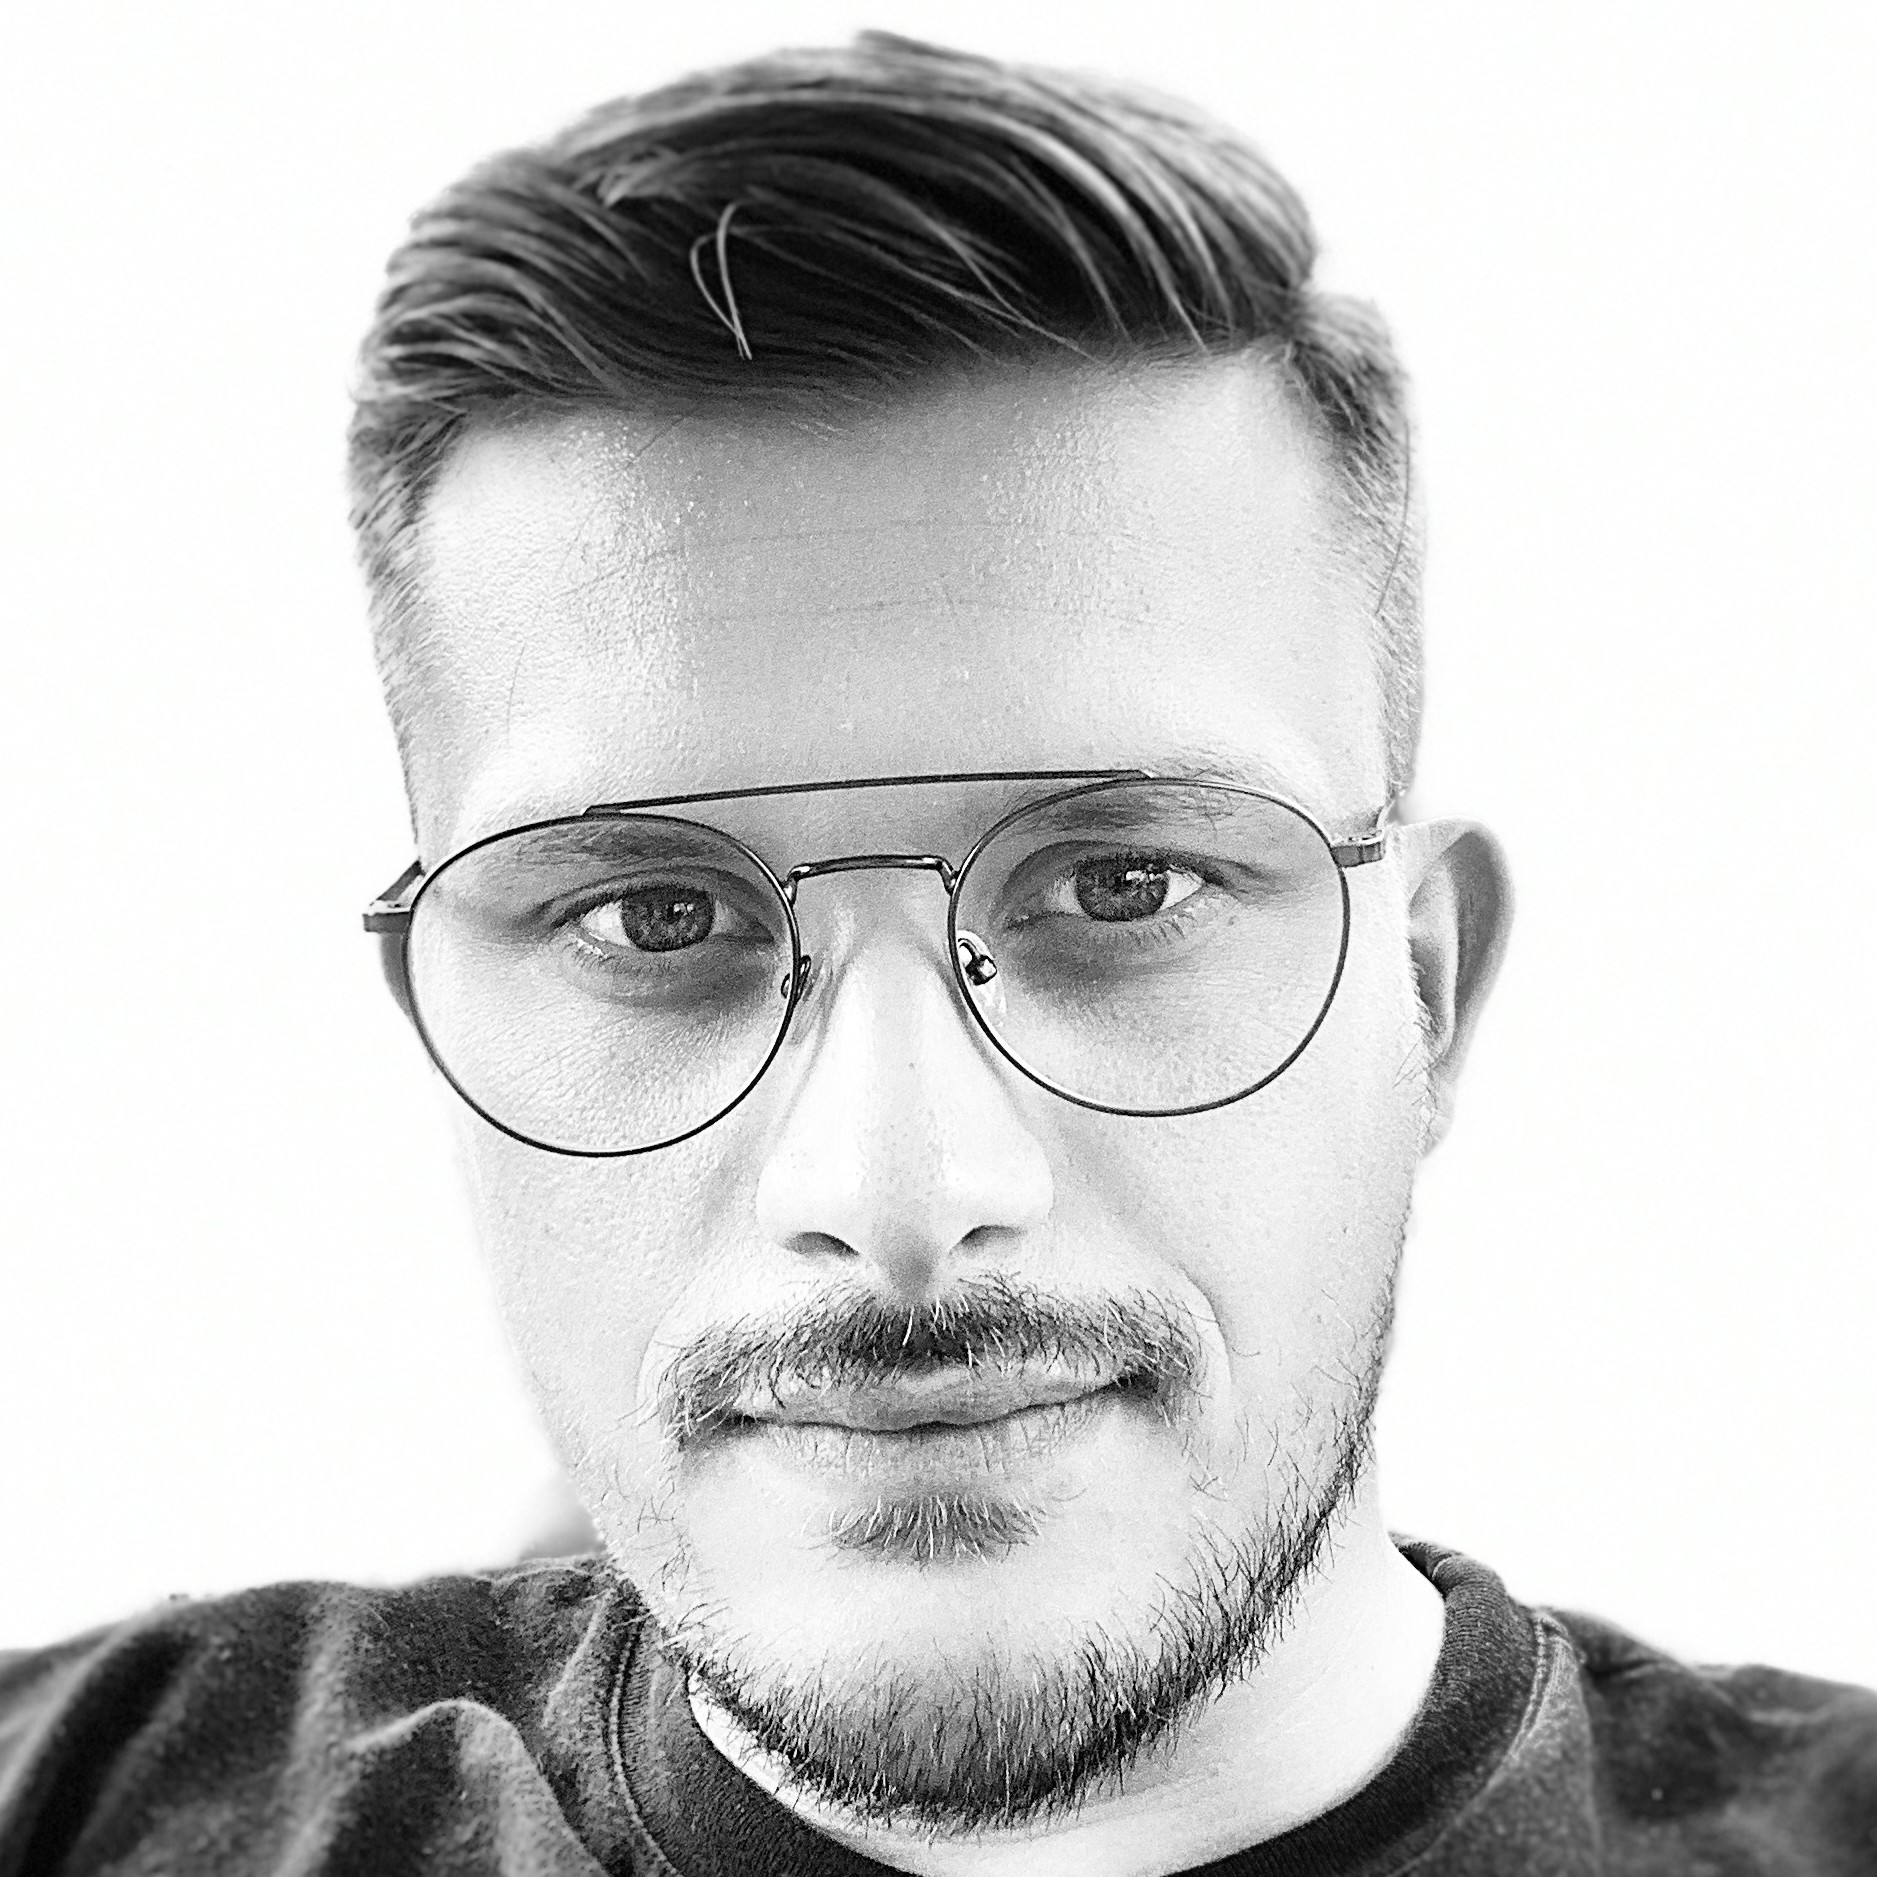
\includegraphics[width=1in,height=1.25in,clip,keepaspectratio]{photos/yohan.jpg}}]{Yohan
        Chatelain} received his Ph.D. degree from the University of Paris-Saclay
    (UVSQ), Versailles, France in 2019. He is a postdoctoral researcher in the
    Big Data Infrastructures for Neuroinformatics lab at the University of
    Concordia, Montreal, Canada. His research topics include computer
    arithmetic, high-performance computing, and reproducibility. Yohan aims at
    democratizing the use of the analysis of stability for scientific computing
    codes through automatic tools to improve numerical quality. 
\end{IEEEbiography}

\vskip -2\baselineskip plus -1fil
\begin{IEEEbiography}[{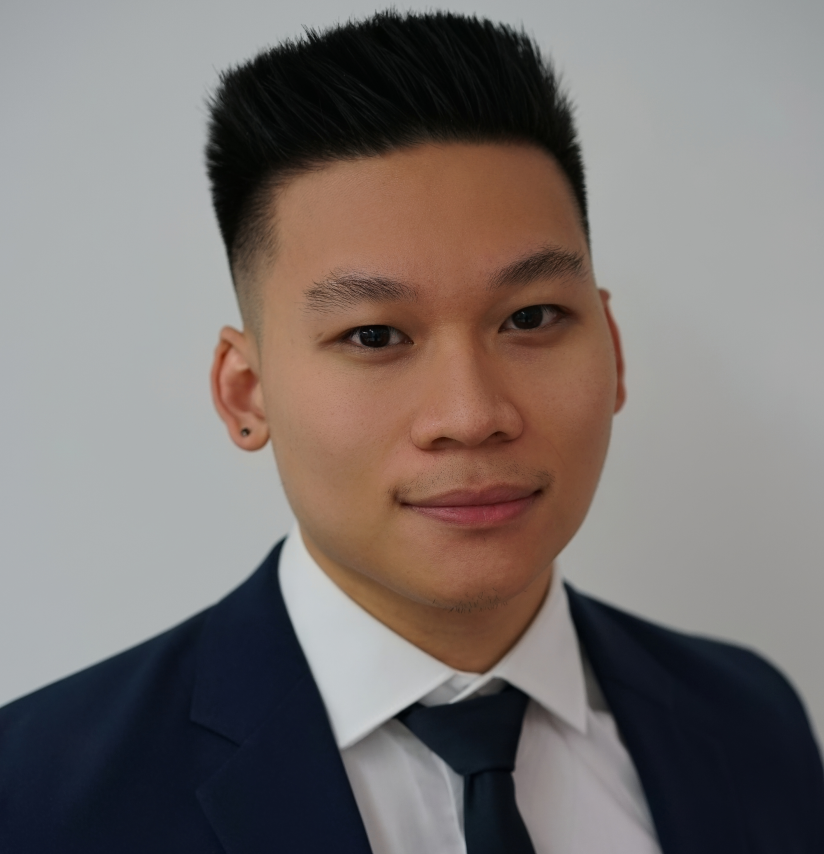
\includegraphics[width=1in,height=1.25in,clip,keepaspectratio]{photos/NigelPhoto.png}}]{Nigel
        Yong Sao Young} was born in Mauritius Island. He is a recent Computer
    Science graduate at Concordia University. He is currently working on his
    software startup, based in the city of Montreal.
\end{IEEEbiography}

%% % if you will not have a photo at all:
\vskip -2\baselineskip plus -1fil
\begin{IEEEbiography}[{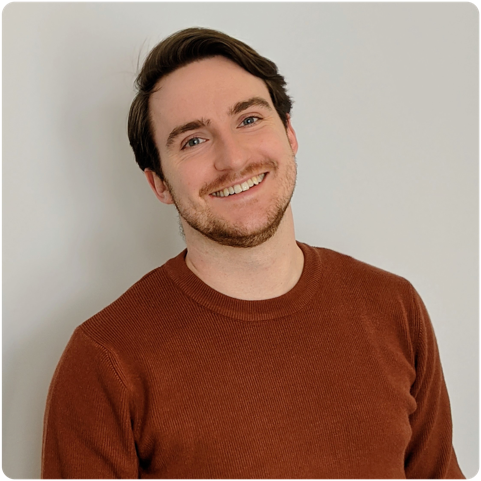
\includegraphics[width=1in,height=1.25in,clip,keepaspectratio]{photos/greg_kiar.png}}]{Gregory
        Kiar} is a research scientist at the Child Mind Institute. Throughout his
    degrees in Biomedical Engineering, Greg has developed techniques to study
    biosignal data, a turn-key tool that allows researchers to generate maps of
    brain connectivity from diffusion MRI data, and techniques to assess and
    improve the stability of research in neuroscience. Greg’s research bridges
    the fields of numerical analysis and brain imaging to evaluate and improve
    the trustworthiness of techniques used to study the brain. 
\end{IEEEbiography}

\vskip -2\baselineskip plus -1fil
\begin{IEEEbiography}[{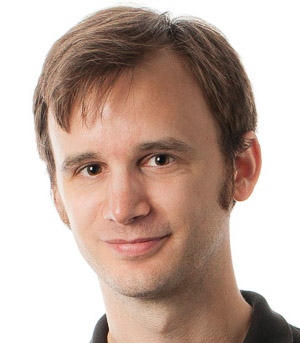
\includegraphics[width=1in,height=1.25in,clip,keepaspectratio]{photos/glatard_tristan.jpg}}]{Tristan
        Glatard} is Associate Professor in the Department of Computer Science and
    Software Engineering at Concordia University in Montreal, and Canada
    Research Chair (Tier II) on Big Data Infrastructures for Neuroinformatics.
    Before that, he was research scientist at the French National Centre for
    Scientific Research and Visiting Scholar at McGill University. 
\end{IEEEbiography}

%% % insert where needed to balance the two columns on the last page with
%% % biographies
%% %\newpage

%% \begin{IEEEbiographynophoto}{Jane Doe}
%% Biography text here.
%% \end{IEEEbiographynophoto}

% You can push biographies down or up by placing
% a \vfill before or after them. The appropriate
% use of \vfill depends on what kind of text is
% on the last page and whether or not the columns
% are being equalized.

%\vfill

% Can be used to pull up biographies so that the bottom of the last one
% is flush with the other column.
%\enlargethispage{-5in}

% \appendix
% 
\section{SciPy}
We tested \pytracer on SciPy examples provided in the tutorial website section.
SciPy is organized in several libraries targeting specific computing domains. We
focused on \texttt{fftpack} (Fast Fourier Transform routines),
\texttt{interpolate} (interpolation and smoothing splines), and
\texttt{optimize} (Optimization and root-finding routines).

\subsection{Interpolation}

This package has five examples: \texttt{interpolation\_1D},
\texttt{multivariate\_data}, \texttt{bspline}, \texttt{spline\_1D} and
\texttt{spline\_2D}.

\texttt{interpolation\_1D} interpolates function $f(x)=\cos(\frac{-x^2}{9})$
with 11 points $x\in[0,10]$. For the five interpolation methods tested (linear,
cubic, nearest, previous, next), the solution found is precise, up to 51 bits
out of the 53 available.

\texttt{multivariate\_data} interpolates the grid $f(x,y)=x(1-x)\cos(4\pi.x)
    \sin(4\pi.y^2)^2$ with $(x,y) \in [0,1] \times [0,1]$. It samples 1,000 points
for each coordinate and uses three interpolation methods: nearest, linear and
cubic. Our results show a precision of 51 bits on average for the three methods.


\texttt{bspline} compares two edge filters: \texttt{bisplev} evaluates a
bivariate B-spline and its derivative whereas \texttt{convolved2d} convolves two
2-dimensional arrays. Figure~\ref{fig:bspline_rr} shows the significant bits,
mean, and standard deviation maps for the two methods as well as the input image
(Fig.~\ref{fig:bspline_original_image}). The middle row shows \texttt{sepfir2d}
results and the bottom row shows \texttt{convol2d} results. Both methods exhibit
similar precision, with 11 significant bits on average. Standard deviations maps
on Figures~\ref{fig:bspline_bisplev_std} and~\ref{fig:bspline_convol2d_std} show
that regions with low spatial frequencies correspond to regions with low
standard deviation, similar to the FFT results. The SciPy tutorial mentions that
\texttt{bisplev} is faster than \texttt{convol2d}. The comparable numerical
precision observed in our experiments reinforce the use of \texttt{bisplev} over
\texttt{convol2d} in this example.

\texttt{spline\_1D} computes the 1D spline interpolation for $f(x)=\sin(x)$ on
points $x=\frac{2\pi k}{8}, k \in [0, 10]$. The spline interpolation uses
\texttt{splrep} to build the spline representation and \texttt{splrev} to
evaluate the spline at any point. It also computes the integral by using
\texttt{splint} and the root finder \texttt{sproot}. Although the traces
diverge, we can analyze the partial aggregation for the \texttt{splrep},
\texttt{splev} and \texttt{splint}. The three functions show results with an
average precision of 51 bits with RR mode.

\texttt{spline\_2D} computes the 2D spline interpolation for function
$z=(x+y)e^{-6(x^2+y^2)}$, with $(x,y) \in [-1,1]\times[-1,1]$ and a sampling of
21 points for each coordinate. \texttt{bisplrep} builds the spline
representation with the $21 \times 21$ points of $z$ over 71 grid sampling
points for $(x,y)$. Figure~\ref{fig:spline2d_rr} shows the results of the spline
evaluation with \texttt{bisplev}.  We observe a significant loss of precision in
places, which follows an interesting pattern that could be further investigated.

\begin{figure}
    \centering
    \begin{subfigure}{.3\linewidth}
        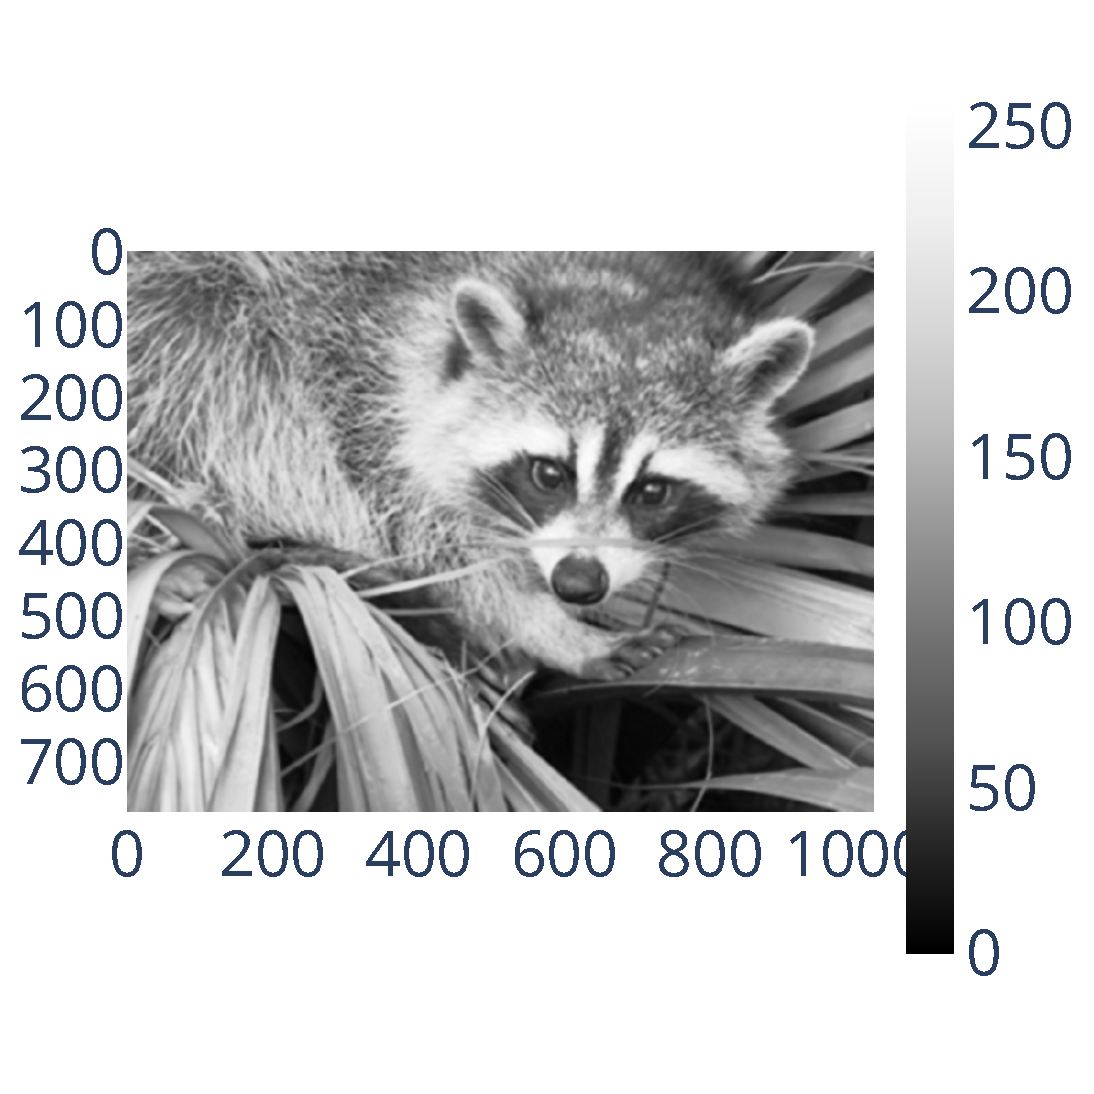
\includegraphics[width=\linewidth]{figure/bspline/original_image.pdf}
        \caption{Original image.}
        \label{fig:bspline_original_image}
    \end{subfigure}\\
    \begin{subfigure}{0.3\linewidth}
        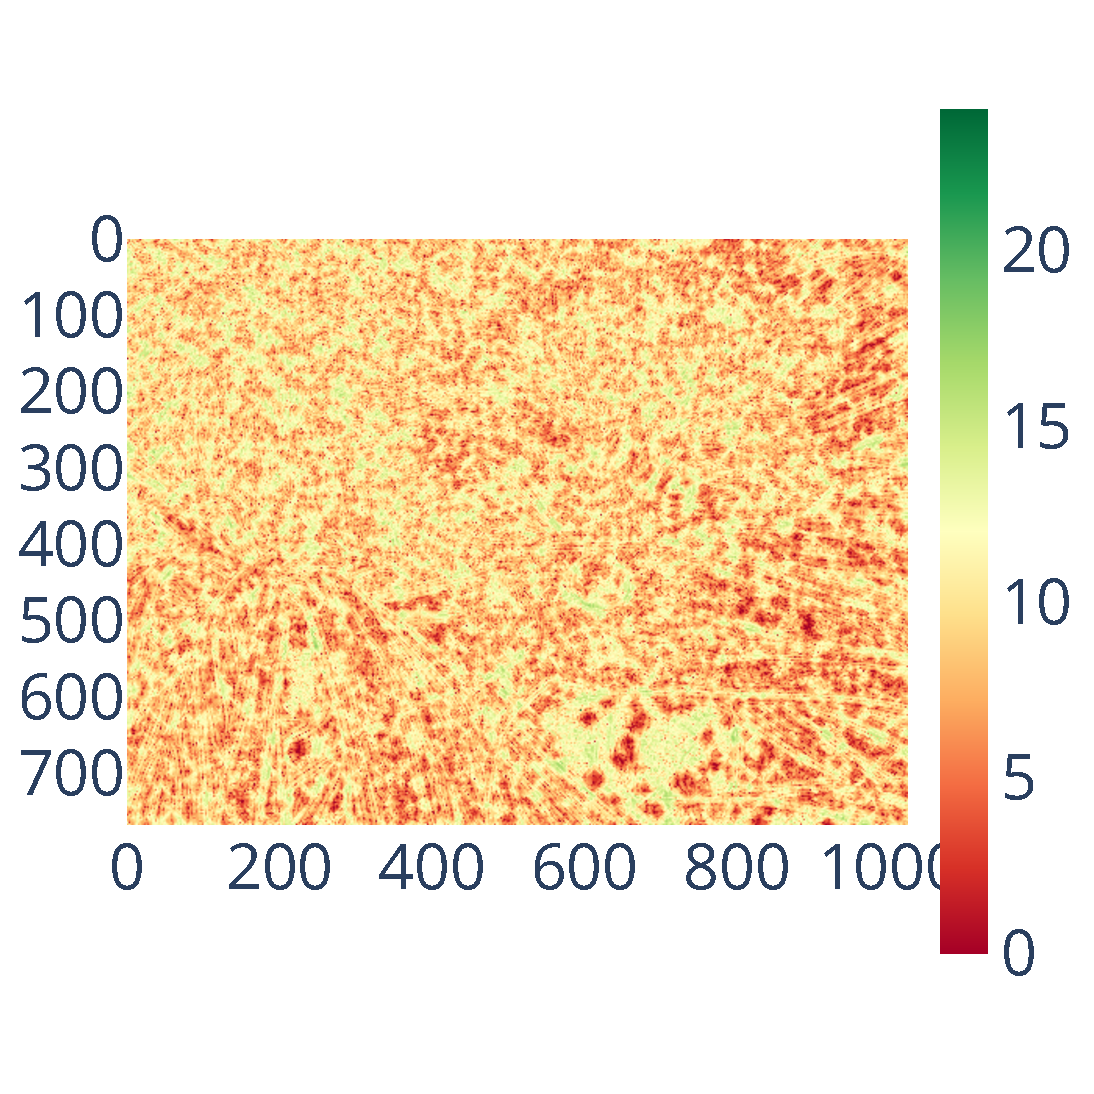
\includegraphics[width=\linewidth]{figure/bspline/bspline_sig.pdf}
        \caption{\centering\texttt{sepfir2d} significant bits}
        \label{fig:bspline_bisplev_sig}
    \end{subfigure}
    \begin{subfigure}{0.3\linewidth}
        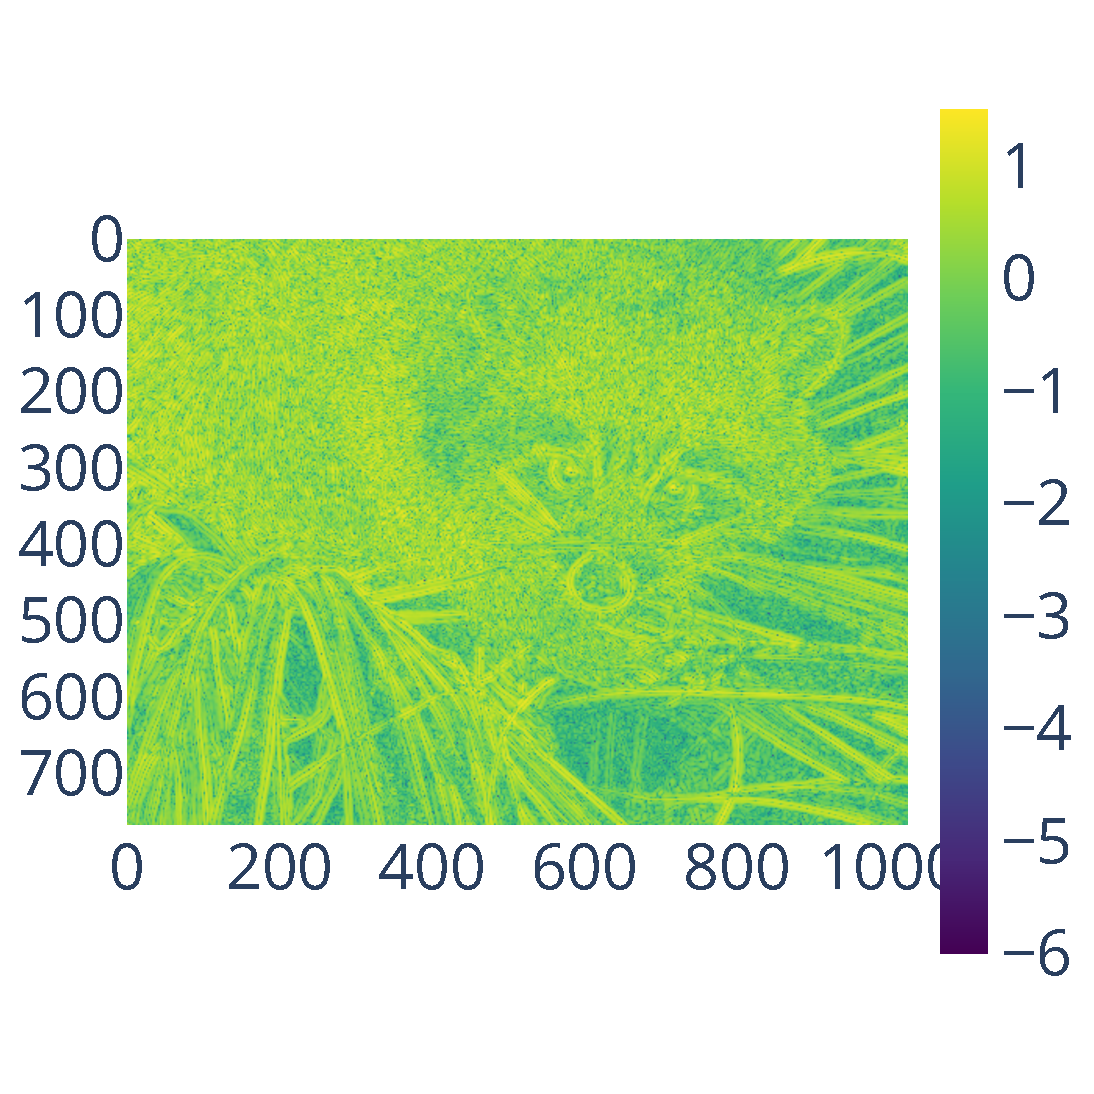
\includegraphics[width=\linewidth]{figure/bspline/bspline_mean_log.pdf}
        \caption{\centering\texttt{sepfir2d} mean (log)}
        \label{fig:bspline_bisplev_mean}
    \end{subfigure}
    \begin{subfigure}{0.3\linewidth}
        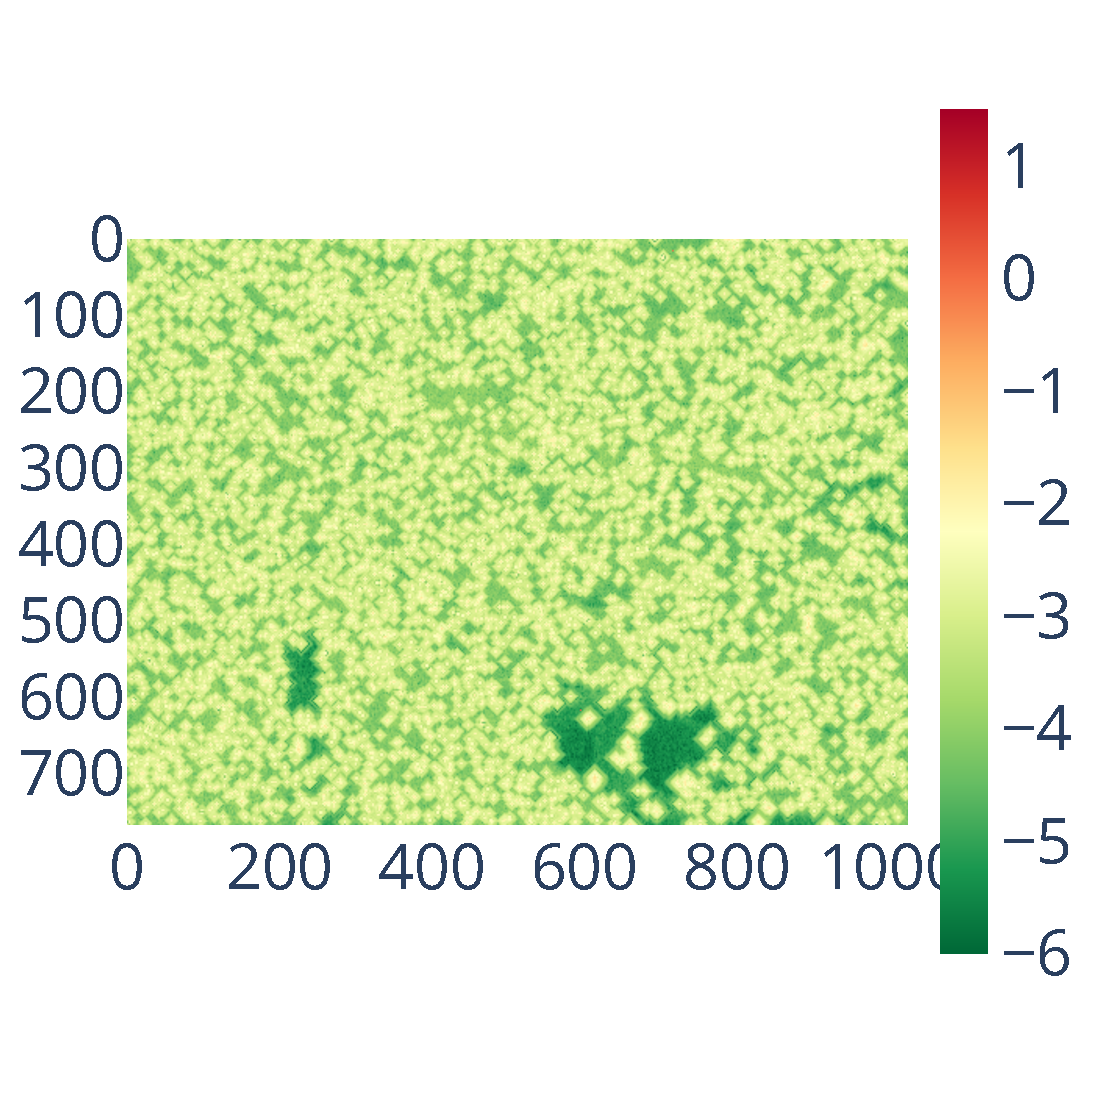
\includegraphics[width=\linewidth]{figure/bspline/bspline_std_log.pdf}
        \caption{\centering\texttt{sepfir2d} standard deviation (log)}
        \label{fig:bspline_bisplev_std}
    \end{subfigure}
    \begin{subfigure}{0.3\linewidth}
        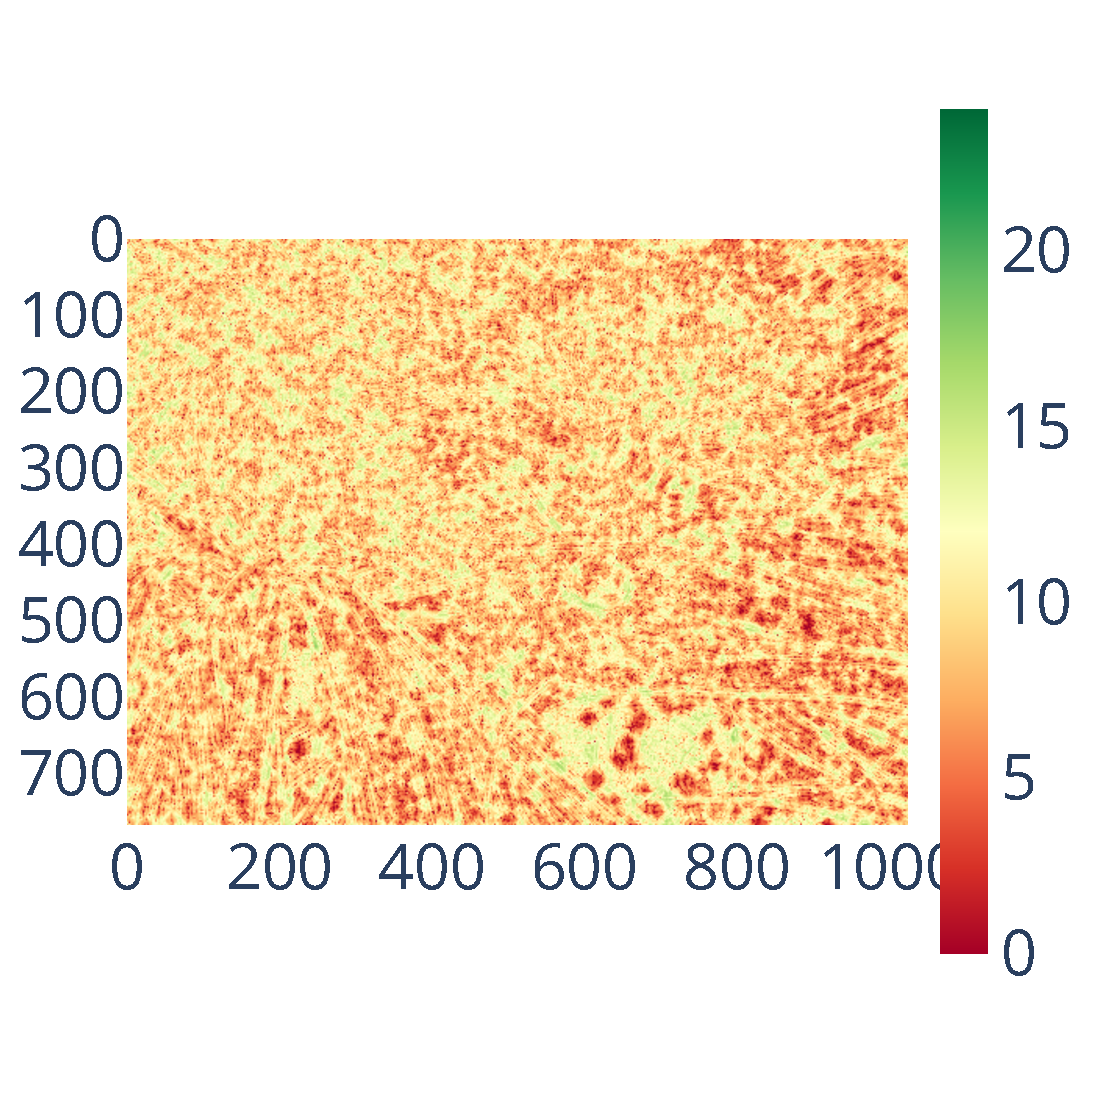
\includegraphics[width=\linewidth]{figure/bspline/convol2d_sig.pdf}
        \caption{\centering\texttt{convol2d} significant bits}
        \label{fig:bspline_convol2d_sig}
    \end{subfigure}
    \begin{subfigure}{0.3\linewidth}
        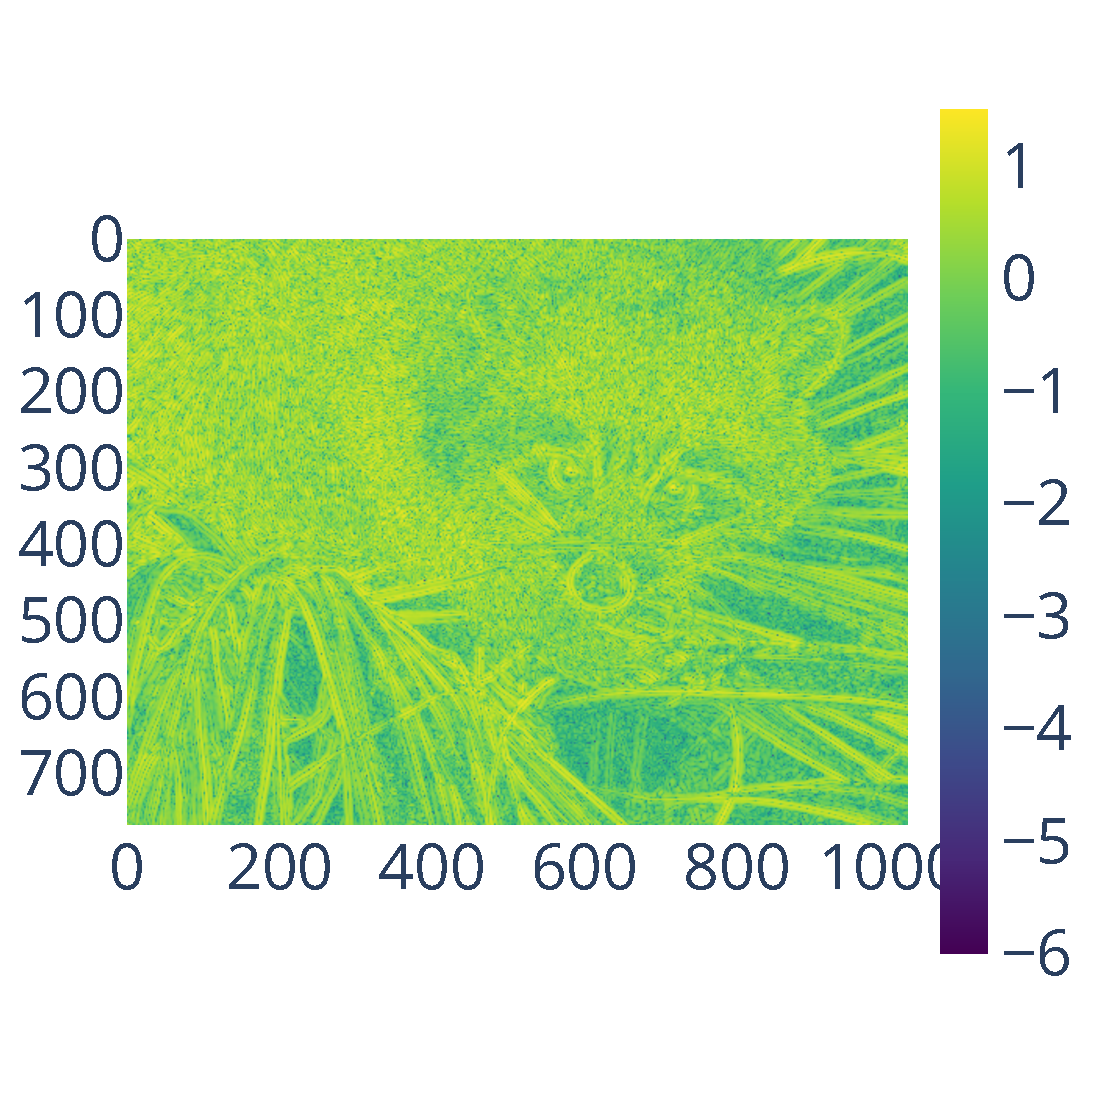
\includegraphics[width=\linewidth]{figure/bspline/convol2d_mean_log.pdf}
        \caption{\centering\texttt{convol2d} mean (log)}
        \label{fig:bspline_convol2d_mean}
    \end{subfigure}
    \begin{subfigure}{0.3\linewidth}
        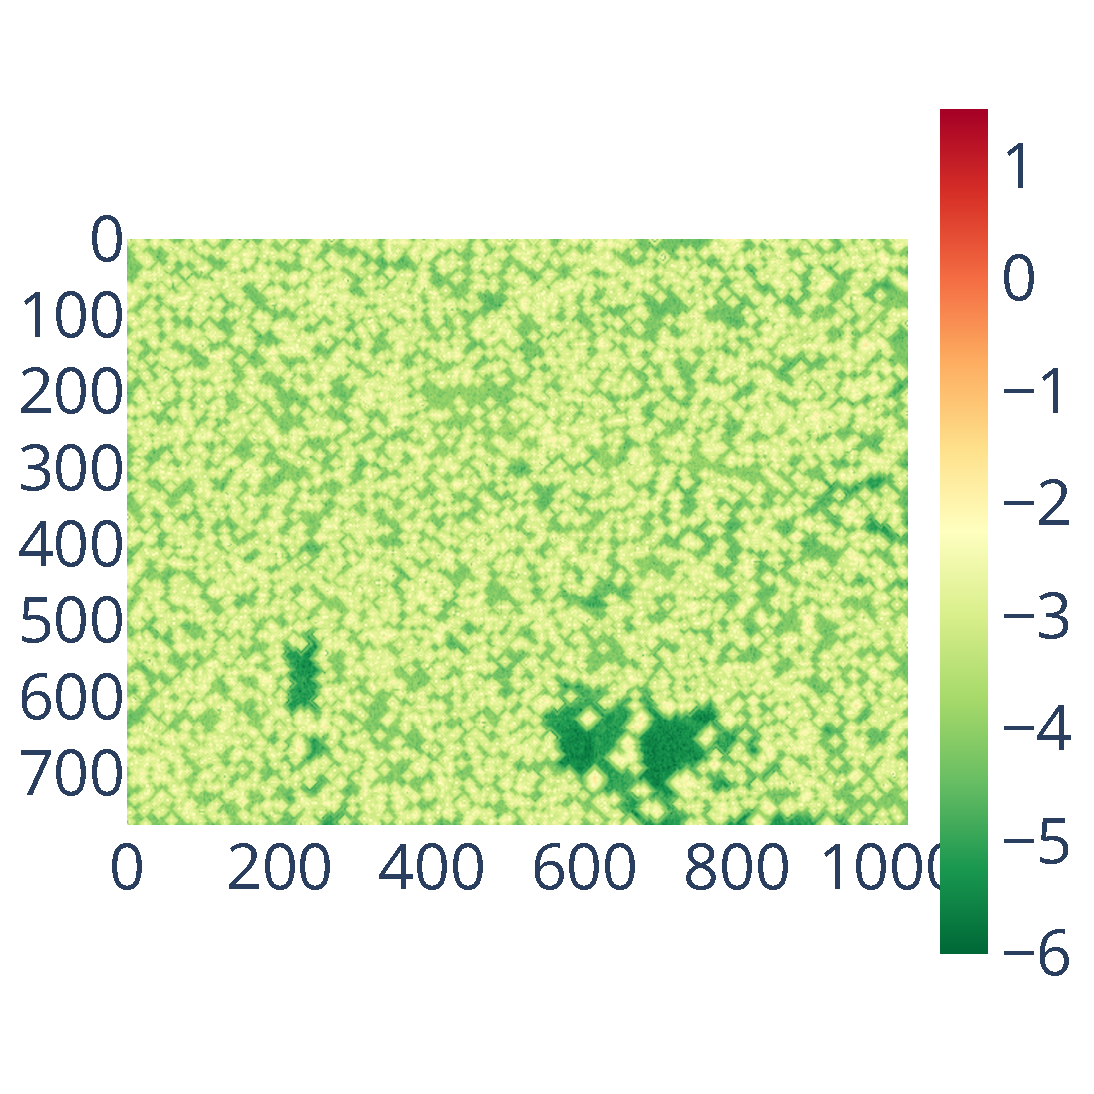
\includegraphics[width=\linewidth]{figure/bspline/convol2d_std_log.pdf}
        \caption{\centering\texttt{convol2d} standard deviation (log)}
        \label{fig:bspline_convol2d_std}
    \end{subfigure}
    \caption{\texttt{bspline} results within RR mode. \texttt{sepfir2d} and
        \texttt{convol2d} have a similar precision.
    }
    \label{fig:bspline_rr}
\end{figure}

\subsection{FFT}

This package has three examples : \texttt{discrete\_cosine\_transform},
\texttt{fft\_1D}, and \texttt{fft\_2D}. All computations are done in double
precision. The results for \texttt{discrete\_cosine\_transform},\texttt{fft\_1D}
and  \texttt{fft\_2D} show precise numerical results with 48 significant bits on
average. We observe that the FFT computation is stable to noisy inputs.
Figures~\ref{fig:fft1D_inputs} (inputs) and~\ref{fig:fft1D_outputs} (outputs)
show the mean and standard deviation of the MCA samples. The three columns
correspond to the FFT computations of:
\begin{enumerate}
    \item $z_1 = \sin(50 . 2\pi . x_i) + \dfrac{1}{2} \sin(80 . 2\pi . x_i),\; x_i = \frac{i}{600},\; i \in [0,600]$
    \item $\mathrm{blackman}(400) \times z_1$
    \item $ z_2= e^{50 . i 2\pi . x_i} + \dfrac{1}{2} e^{-80 . i2\pi .x_i },\; x_i = \frac{i}{800},\; i \in [0,400] $
\end{enumerate}

\add{The} top row in Figures~\ref{fig:fft1D_inputs} and~\ref{fig:fft1D_outputs} show the
input mean value while the bottom row shows the standard deviation. The points
with low magnitude in Figure~\ref{fig:fft1D_inputs} correspond to inputs near 0
when the input of $\sin$ or $\exp$ is close to $k\pi$, $k \in \mathbb{Z}$.
Indeed, since MCA introduces a slight noise, the result is not exactly 0. We can
see in Figure~\ref{fig:fft1D_inputs} that the maximal noise introduced by MCA on
the inputs is in the order of $10^{-14}$, two orders of magnitude higher than
the $ulp \simeq 10^-16$ for double precision. This slight noise introduced can
be interpreted as white noise on the input signal. We can see on the bottom row
of Figure~\ref{fig:fft1D_outputs} that the frequency noise is of the same order
of of magnitude as the input noise, which is expected. The two peaks at x=38 and
x=562 corresponds to the actual frequencies of the input signal.

\subsection{Optimization}

This package has eleven examples. Seven examples involve the same optimization
problem solved with and without constraints using different methods. One example
optimizes a chemical problem under constraints. The last three examples solve a
different problem each.

\subsubsection{Unconstrained minimization of multivariate scalar functions}
Four Quasi-Newton-Raphson methods minimize function $f$ by using Newton's step:
$x_{k+1} = x_{k} - B^{-1}(x_k)\nabla f(x_k)$, where $\nabla$ and $B$ are the
gradient and the approximation of the Hessian matrix of $f$. The
\texttt{Broyden-Fletcher-Goldfarb-Shanno}~\cite{BFGS} (BFGS) and
\texttt{Newton-Conjugate-Gradient}~\cite{nocedal2006numerical} (NCG) are line
search methods that approximate $H$ by adding two symmetric rank-one matrices
and by using the Conjugate-Gradient method. The \texttt{Trust-Region Truncated
    Generalized Lanczos / Conjugate Gradient}~\cite{gould1999solving} (TR-Krylov),
\texttt{Trust-Region Newton-Conjugate-Gradient} (TR-NCG), and
\texttt{Trust-Region Nearly Exact}~\cite{nocedal2006numerical} (TR-Exact) are
trust-region methods approximating $H$ by solving the trust-region subproblem
restricted to a truncated Krylov subspace and by solving nonlinear equations for
each quadratic subproblem. In addition, the
\texttt{Nelder-Mead}~\cite{singer2009nelder} simplex-based method iteratively
transforms a simplex until its vertices are getting closer to a local minima of
the function. All methods are applied to the Rosenbrock function.

\paragraph{Constrained minimization of multivariate scalar functions}
Two optimizers solve an optimization problem by taking into account constraints.
The \texttt{Sequential Least SQuares Programming} uses the
SLSQP~\cite{kraft1988software} method to optimize the Rosenbrock function. The
\texttt{Least-squares minimization} uses the Trust Region Reflective
algorithm~\cite{li1993centering} to solve a fitting problem from an enzymatic
reaction.

The SLSQP and unconstrained minimization methods minimize the
\textbf{Rosenbrock} function of $N$ variables that reaches its minimum (0) when
$x_i=1,\; \forall i \leq N-1$:
$f(x) = \sum_{i=1}^{N-1} 100(x_{i+1}-x^2_i)^2 + (1-x_i)^2$.
Figure~\ref{fig:unconstrained_optimization} shows the number of significant bits
of the solution for the different methods used. The $(p)$ notation for the NCG,
Trust-Krylov, and Trust-NCG methods in the legend refers to the variant where
the Hessian matrix is replaced by a function computing the matrix-vector product
of the Hessian and an arbitrary vector, to save memory and time. All the methods
have a good precision ranging from 43 to 53 significant bits. The Nelder-Mead
method is the least precise one with $\simeq$ 43 significant bits on average,
while the Trust-Region-Newton-CG is the most precise one with $\simeq$ 53
significant bits, the highest precision achievable in double precision. The
remaining methods have a similar precision.

The SLSQP also minimizes the Rosenbrock function with the following constraint:
$x_0$ + $2x_1$ $\leq$ 1
$x_0^2$ + $x_1$ $\leq$ 1
$x_0^2$ - $x_1$ $\leq$ 1
$2x_0$ + $x_1$ = 1
0 $\leq$ $x_0$ $\leq$ 1
-0.5 $\leq$ $x_1$ $\leq$ 2.
% \begin{eqnarray*}
%     x_0 + 2x_1 \leq 1 \\
%     x_0^2 + x_1 \leq 1 \\
%     x_0^2 - x_1 \leq 1 \\
%     2x_0 + x_1 = 1 \\
%     0 \leq x_0 \leq 1 \\
%     -0.5 \leq x_1 \leq 2 
% \end{eqnarray*}
The problem has a unique solution $[x_0, x_1] = [0.4149, 0.1701]$. Results
obtained with RR show a precision of 47 and 44 significant bits for the first
and the second solution. %\tristan{which method is tested?}.

The \texttt{least-square minimization} example solves a fitting problem from an enzymatic reaction~\cite{kowalik1968analysis} with 11 residuals defined as:
\begin{eqnarray*}
    f_i(x) &=& \frac{x_0(u_i^2 + u_ix_1)}{u_i^2 + u_ix_2+x_3}-y_i,\; i=0,...,10 \\
    &0& \leq x_j \leq 100,\; j=0,..,3
\end{eqnarray*}
where where $y_i$ are measurement values, $u_i$ are values of the independent
variable, and $x_i$ the unknown. Results within RR show a precision of 51, 46,
47, and 48 significant bits for each component of the solution
respectively.% \tristan{which solver is used?}.

\subsubsection{Root finding}
% We tested three root finder algorithms with one for small problems using the hybrid Powell and Levenberg-Marquardt methods  (\texttt{root\_finding}) and two for large problems using a Krylov approximation for the inverse Jacobian with and without the help of a preconditioner (\texttt{root\_finding\_large\_preconditionned} and \texttt{root\_finding\_large}).

The \texttt{root\_*} examples use three algorithms to find the root of
non-linear equations. \texttt{root\_finding} uses the hybrid Powell method to
solve a single-variable transcendental equation and the Levenberg-Marquardt
method for a set of non-linear equations. \texttt{root\_finding\_large} and
\texttt{root\_finding\_large\_preconditioned} examples use the Krylov method to
approximate the inverse Jac\add{o}bian with and without the help of a preconditioner.
They solve an integrodifferential equation on a square $(x,y) \in [0,1] \times
    [0,1]$, $P(x,1)=1$, and $P=0$ elsewhere on the boundary. The function $P$ is
discretized with a Cartesian grid $P_{n,n}=P(nh,nh)$, with $n=75$, and its
derivatives are approximated by $\partial_x^2P(x,y) \simeq (P(x+h,y) - 2P(x,y) +
    P(x-h,y))/h^2$.

% the two following equations: $x + 2\cos(x) = 0$ and 
% the set $x_0\cos(x_1)=4$; $x_0x_1-x_1 = 5$ while the 
% \texttt{root\_finding\_large} and \texttt{root\_finding\_large\_preconditioned} tests 
% solve the equation:
% \[
%     (\partial_x^2 + \partial_y^2)P + 5 \left(\int_0^1 \int_0^1 cosh(P)\, dx dy \right)^2 = 0
% \]

All the examples diverge even within RR, which is not surprising since
root-finding methods can easily take a few extra steps to find the root
depending on the starting point. Nevertheless, for the
\texttt{root\_finding\_large} example, 3 traces among the 5 samples can be
merged for both RR and MCA modes. Figure~\ref{fig:root_finding_large} shows the
mean and standard deviation of the result for these 3 samples. We can see that a
similar solution was found for RR and Full MCA. Full MCA leads to a lower
precision than RR although both standard deviation maps remain in the same order
of magnitude. Finally, it is interesting to note the impact of preconditioning
on the result numerical quality: as Table~\ref{tab:pytracer_results_summary}
shows, the precision doubles between \texttt{root\_finding\_large} and
\texttt{root\_finding\_large\_preconditioned}.

\begin{figure}
    \centering
    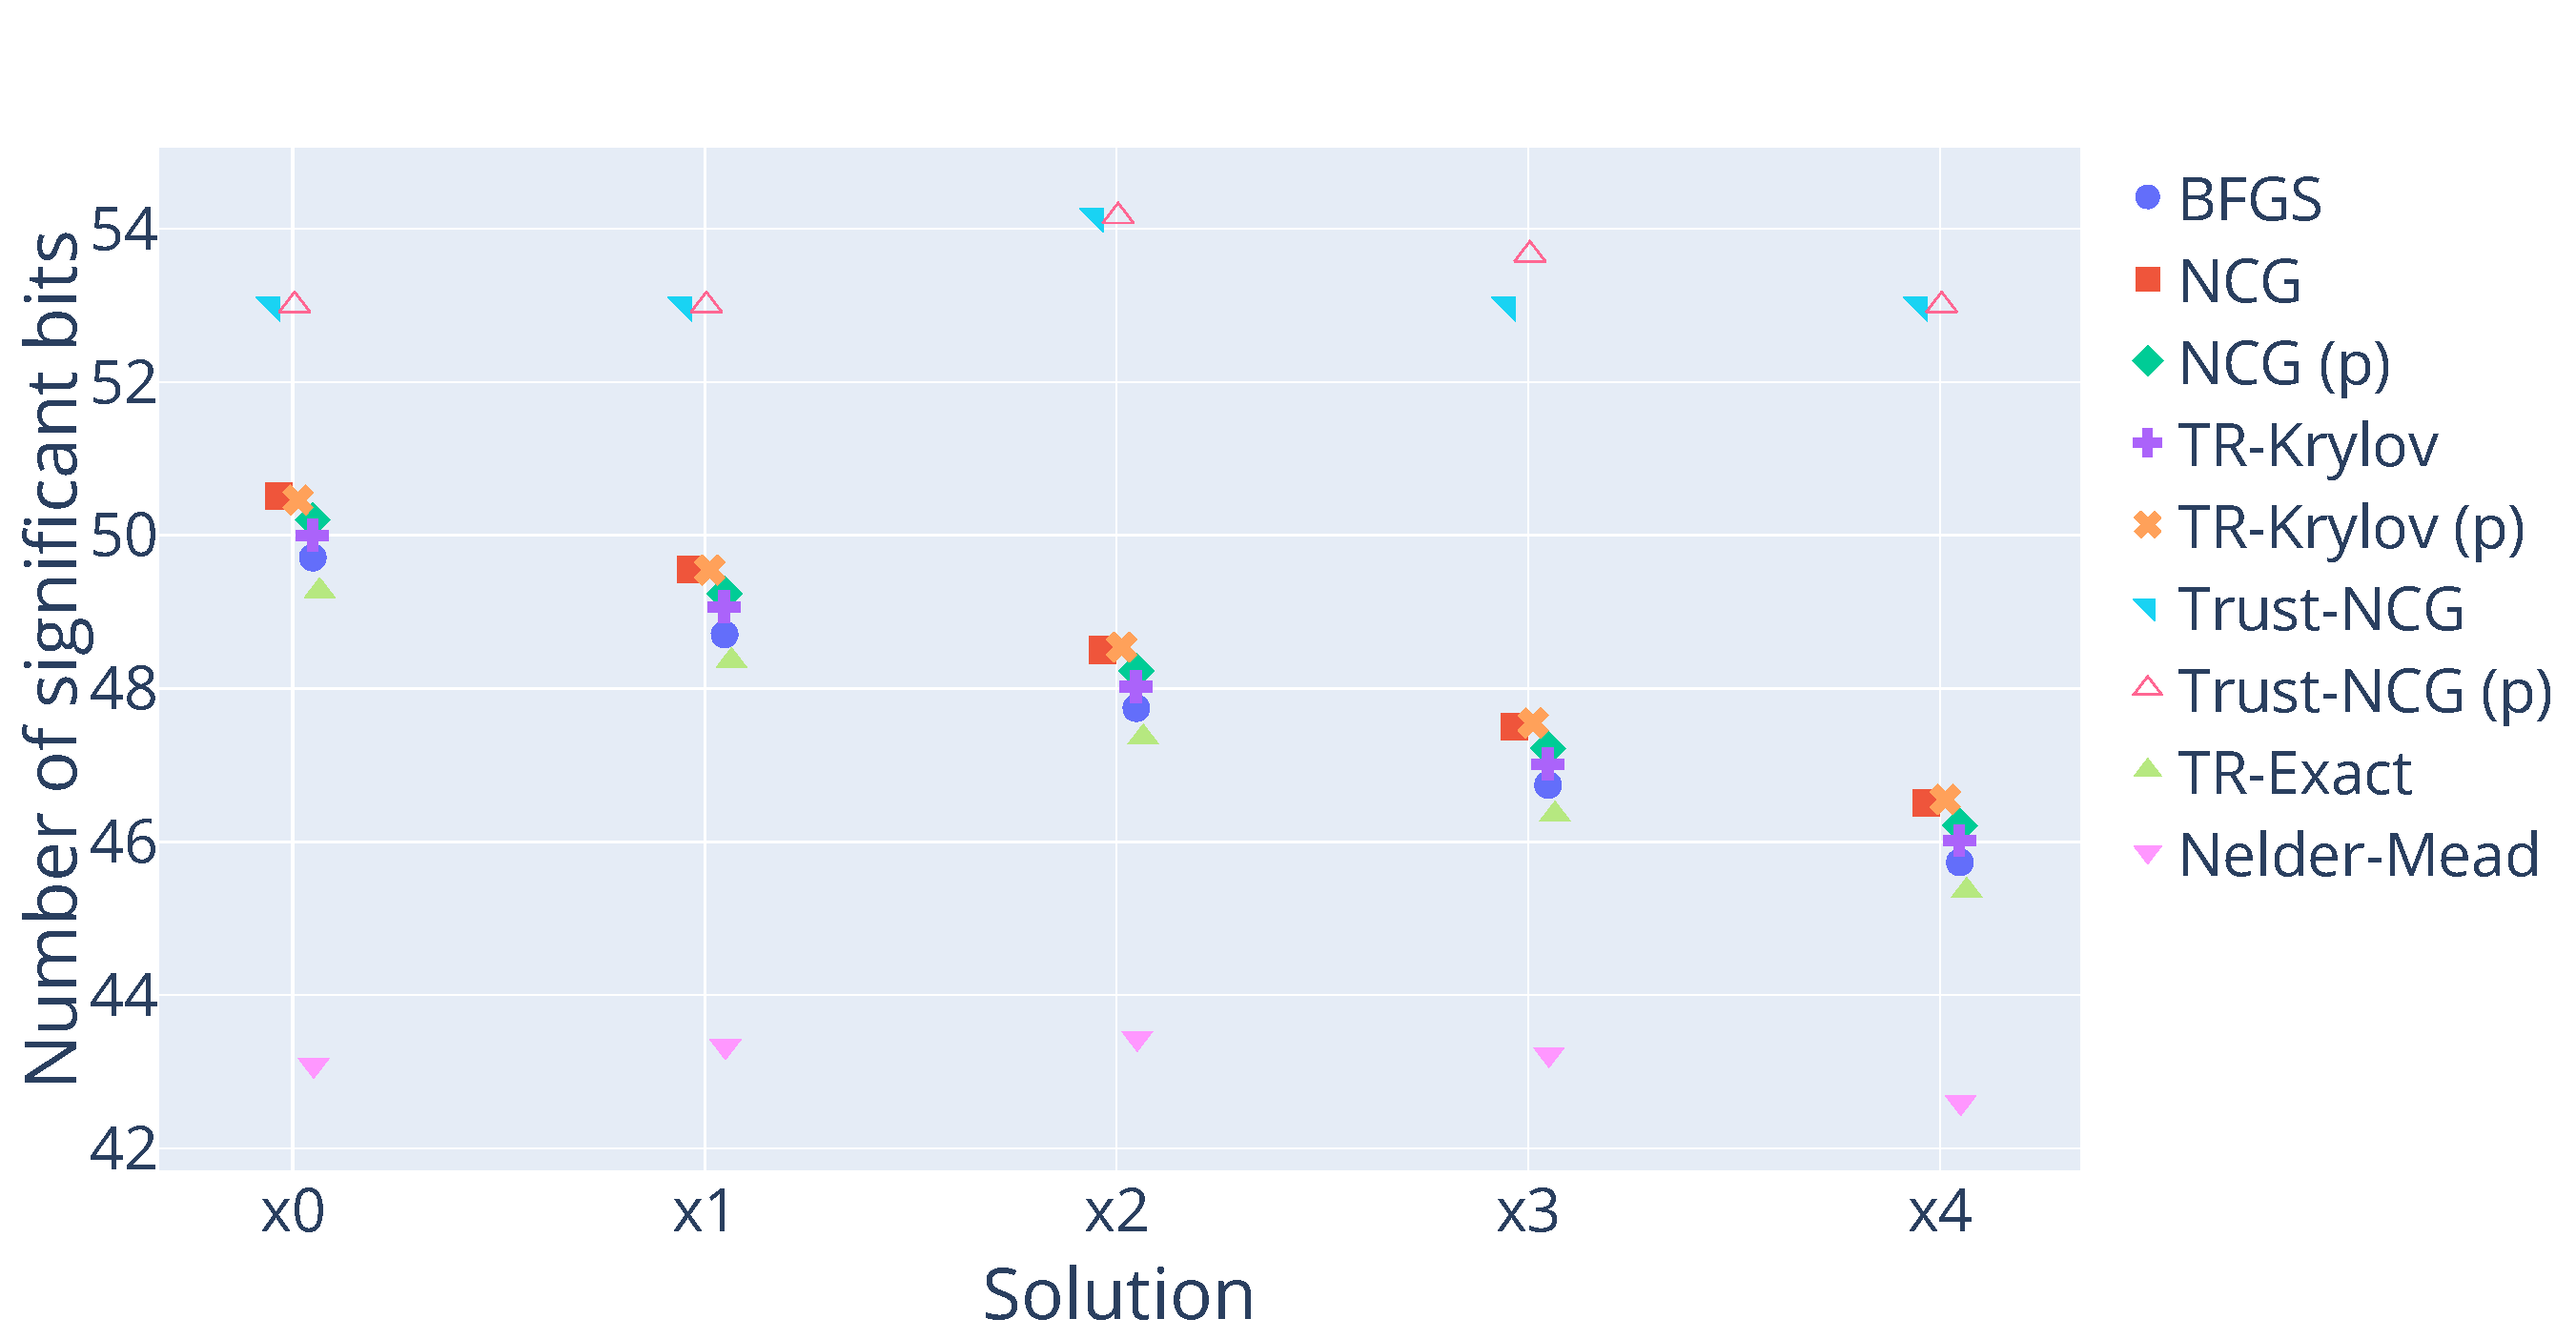
\includegraphics[width=\linewidth]{figure/unconstrained_optimization_comparison.pdf}
    \caption{Comparison of results precision for different optimization solvers within RR mode.}
    \label{fig:unconstrained_optimization}
\end{figure}

\begin{figure}
    \centering
    \begin{subfigure}{0.45\linewidth}
        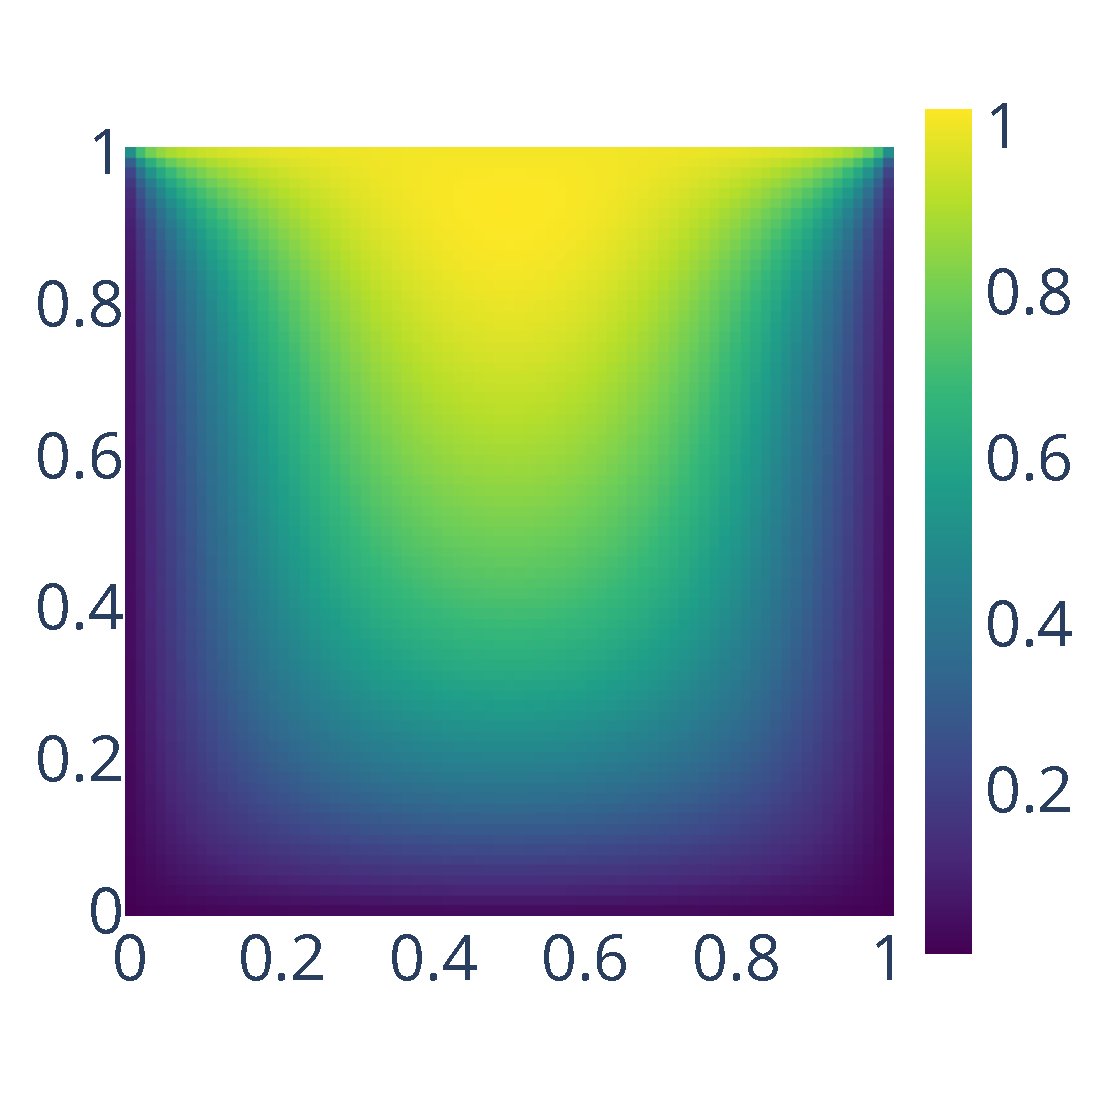
\includegraphics[width=\linewidth]{figure/root_finding/solution_mean_RR.pdf}
        \caption{Mean solution (RR)}
        \label{fig:mean_solution_rr}
    \end{subfigure}
    \begin{subfigure}{0.45\linewidth}
        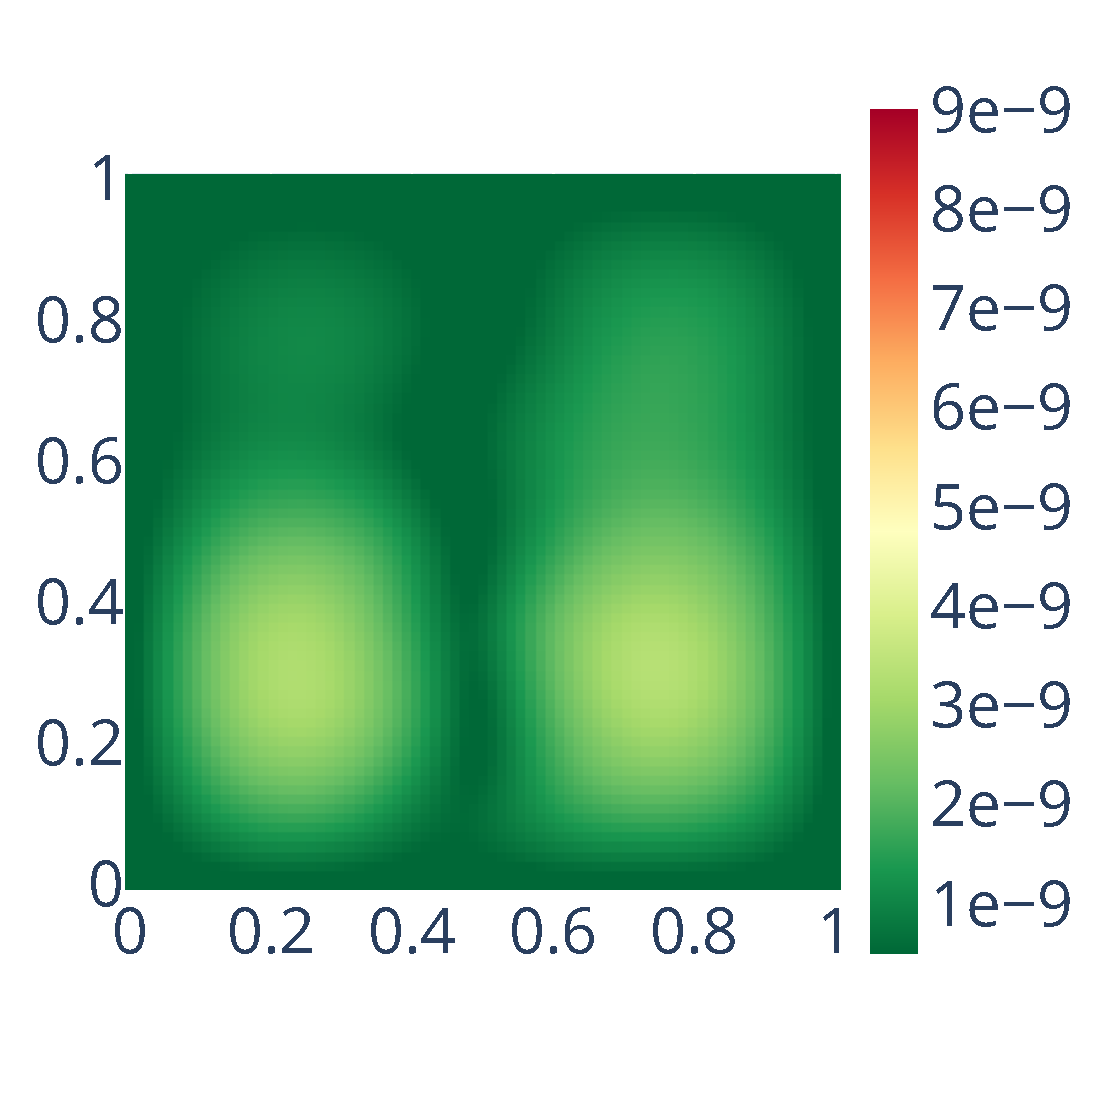
\includegraphics[width=\linewidth]{figure/root_finding/solution_std_RR.pdf}
        \caption{Standard deviation solution (RR)}
        \label{fig:stdev_rr}
    \end{subfigure}

    \begin{subfigure}{0.45\linewidth}
        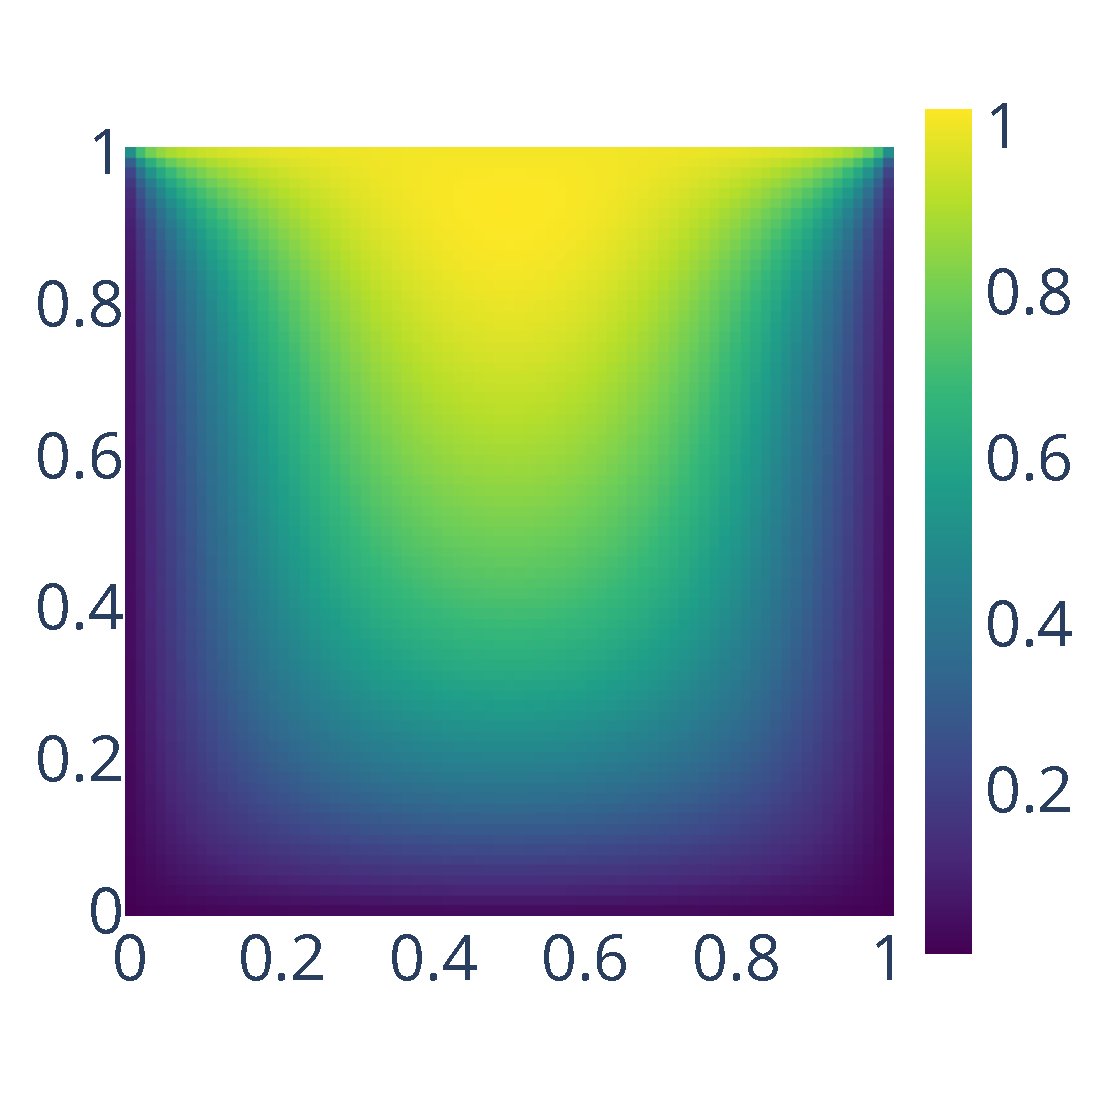
\includegraphics[width=\linewidth]{figure/root_finding/solution_mean_MCA.pdf}
        \caption{Mean solution (Full MCA)}
        \label{fig:mean_solution_mca}
    \end{subfigure}
    \begin{subfigure}{0.45\linewidth}
        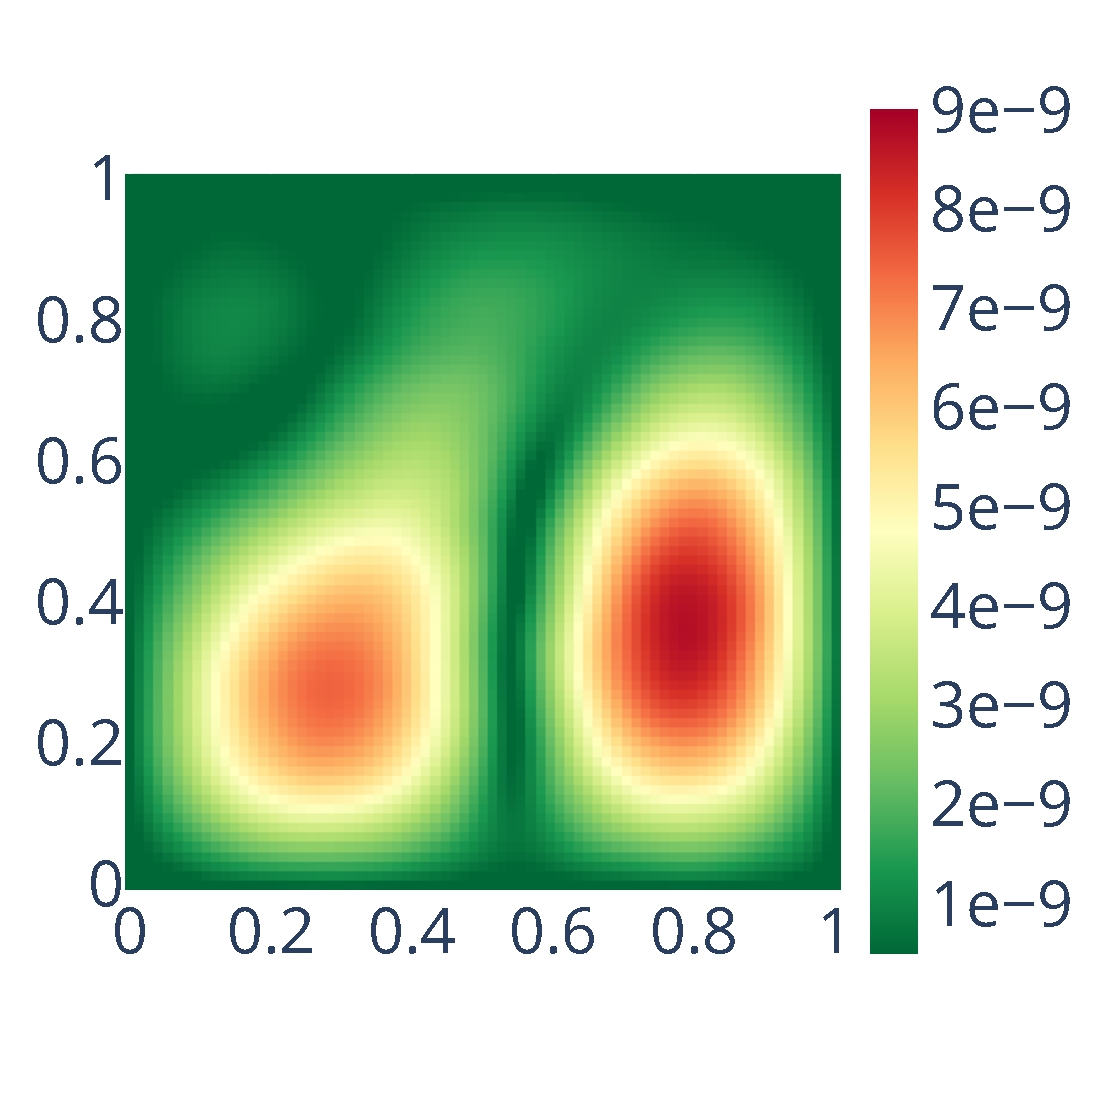
\includegraphics[width=\linewidth]{figure/root_finding/solution_std_MCA.pdf}
        \caption{Standard deviation (Full MCA)}
        \label{fig:stdev_mca}
    \end{subfigure}
    \caption{Solution of \texttt{root\_finding\_large} example.
        The standard deviation has two maximum for both RR and Full MCA modes. The standard deviation remains lower than
        the stopping criterion threshold fixed at $6.10^{-6}$. }
    \label{fig:root_finding_large}
\end{figure}

\subsection{Scikit learn}
\label{sec:sklearn_tests}

Scikit-learn offers a well-supplied and documented list of examples that
facilitates its use with Pytracer. Among the several available examples, we
choose the following representative set listed in
Table~\ref{tab:pytracer_results_summary}. The following paragraphs focus on the
most interesting stability results observed across all experiments.

\subsubsection{Separating hyperplane}

This example uses a linear Support Vector Machine (SVM) classifier trained using
the Stochastic Gradient Descent (SGD) method to find the maximum separating
hyperplane between sets of 2D points. The example trains the SVM with 50 random
points separated in 2 clusters with hyperparameter $\alpha=0.01$ and using the
hinge loss function. Once the model is trained, the example generates a
$[-1,5]\times[-1,5]$ Cartesian grid discretized with 100 points and predicts the
class label for each point with integer coordinates.
Figure~\ref{fig:hyperplan_sig_zoom} shows the number of significant bits
obtained with RR for each point of the grid.
We can see that yellow regions
close to the separating hyperplane are highly unstable with a number of
significant bits below 0, meaning that the classifier is unsure about the
predicted class.
%\tristan{Describe and comment on the other 2 tests, why are they more stable? Is it because the training set has more points?}


% \begin{figure}
%     \centering
%     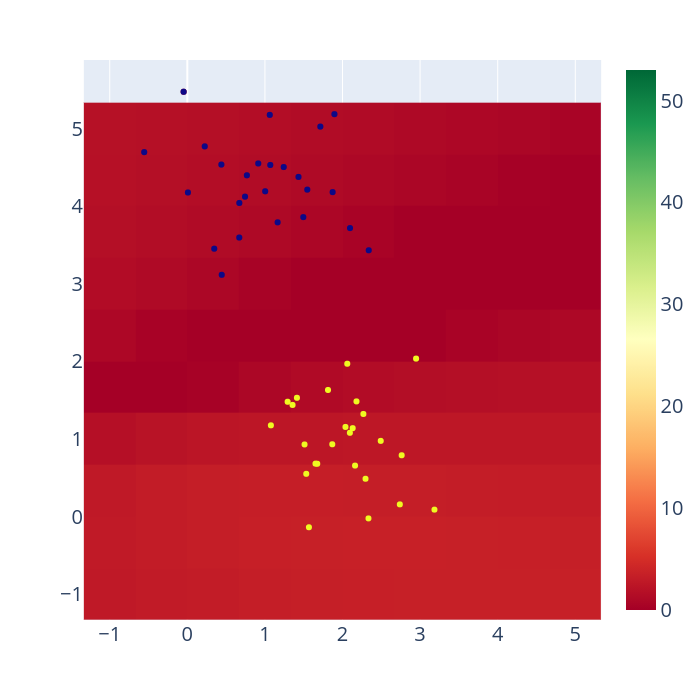
\includegraphics[width=\linewidth]{figure/separating_hyperplan/hyperplan.png}
%     \caption{Ratio $mean/std$ of Separating hyperplane test result within RR mode.
%     Circle and square points represent respectively the train and test dataset.
%     The color represents the predicted class. We can see that 
%     instability is high around the hyperplane which is coherent with 
%     the fact the classifier has difficulty to decide in which side of the hyperplane the 
%     point is.}
%     \label{fig:separating_hyperplan}
% \end{figure}

\begin{figure}
    \centering
    % \begin{subfigure}{.3\linewidth}
    % 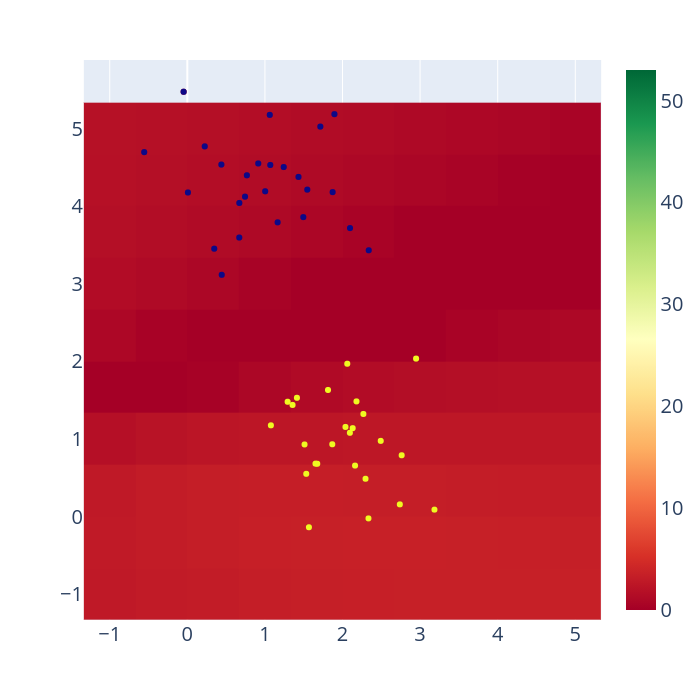
\includegraphics[width=\linewidth]{figure/separating_hyperplan/hyperplan.png}
    % \caption{}
    % \label{fig:hyperplan_sig}
    % \end{subfigure}
    \begin{subfigure}{.45\linewidth}
        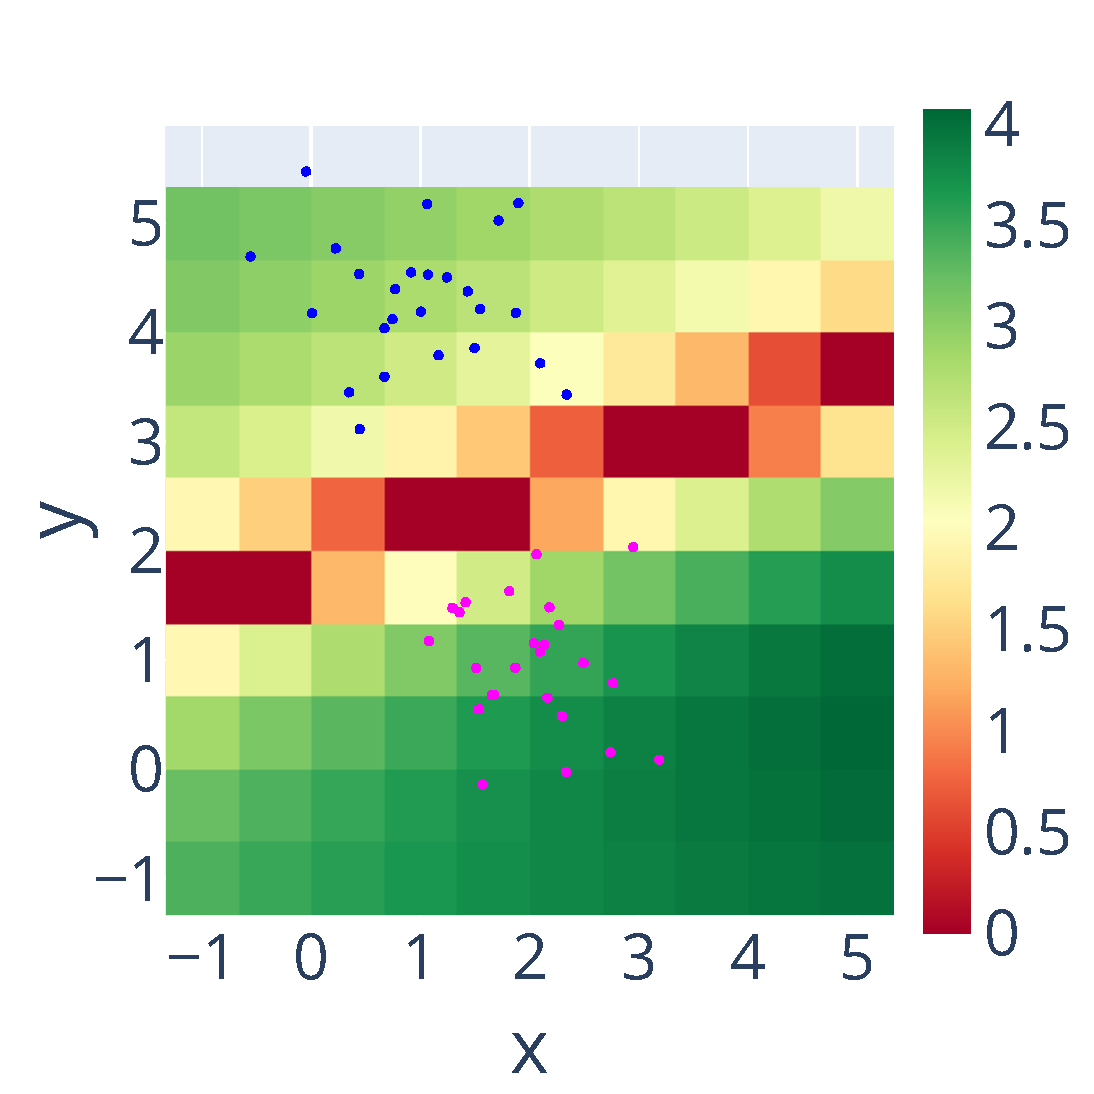
\includegraphics[width=\linewidth]{figure/separating_hyperplan/hyperplane_zoom.pdf}
        \caption{Separating hyperplane}
        \label{fig:hyperplan_sig_zoom}
    \end{subfigure} \\
    \begin{subfigure}{.45\linewidth}
        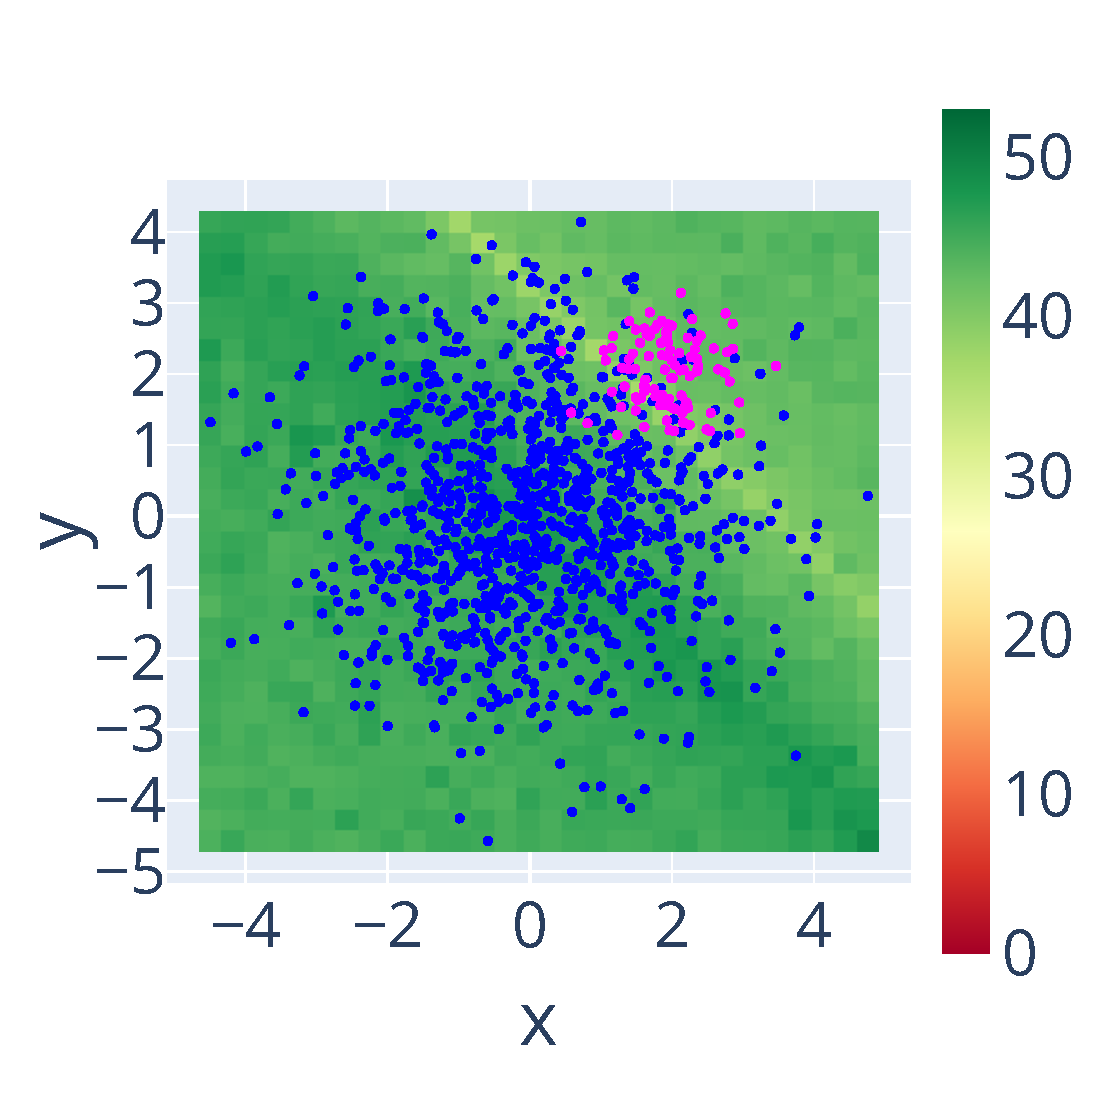
\includegraphics[width=\linewidth]{figure/SVM/non_weighted.pdf}
        \caption{SVM (non weighted)}
        \label{fig:SVM_nw_sig}
    \end{subfigure}
    \begin{subfigure}{.45\linewidth}
        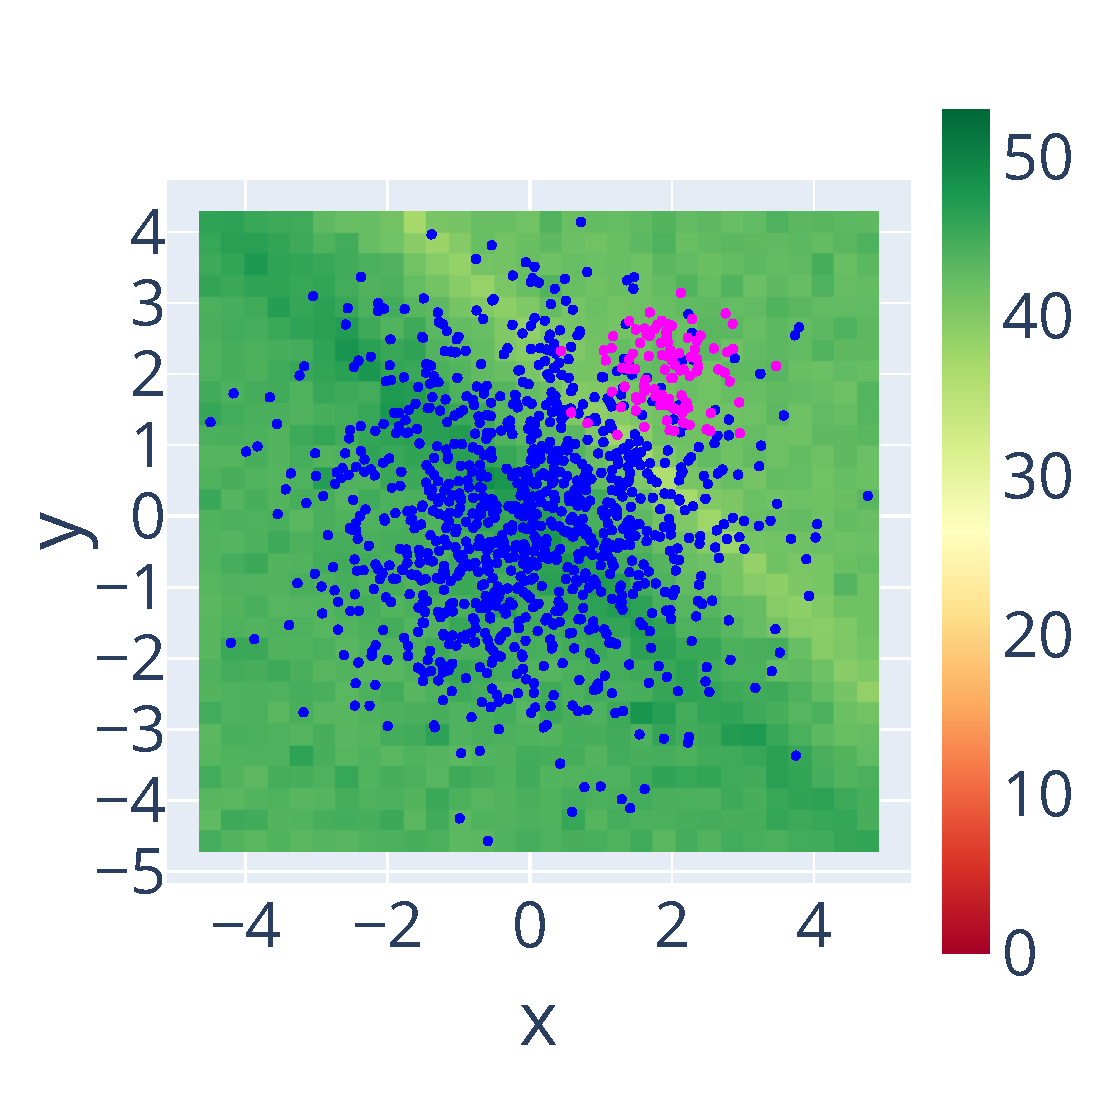
\includegraphics[width=\linewidth]{figure/SVM/weighted.pdf}
        \caption{SVM (weighted)}
        \label{fig:SVM_w_sig}
    \end{subfigure} \\
    \begin{subfigure}{.45\linewidth}
        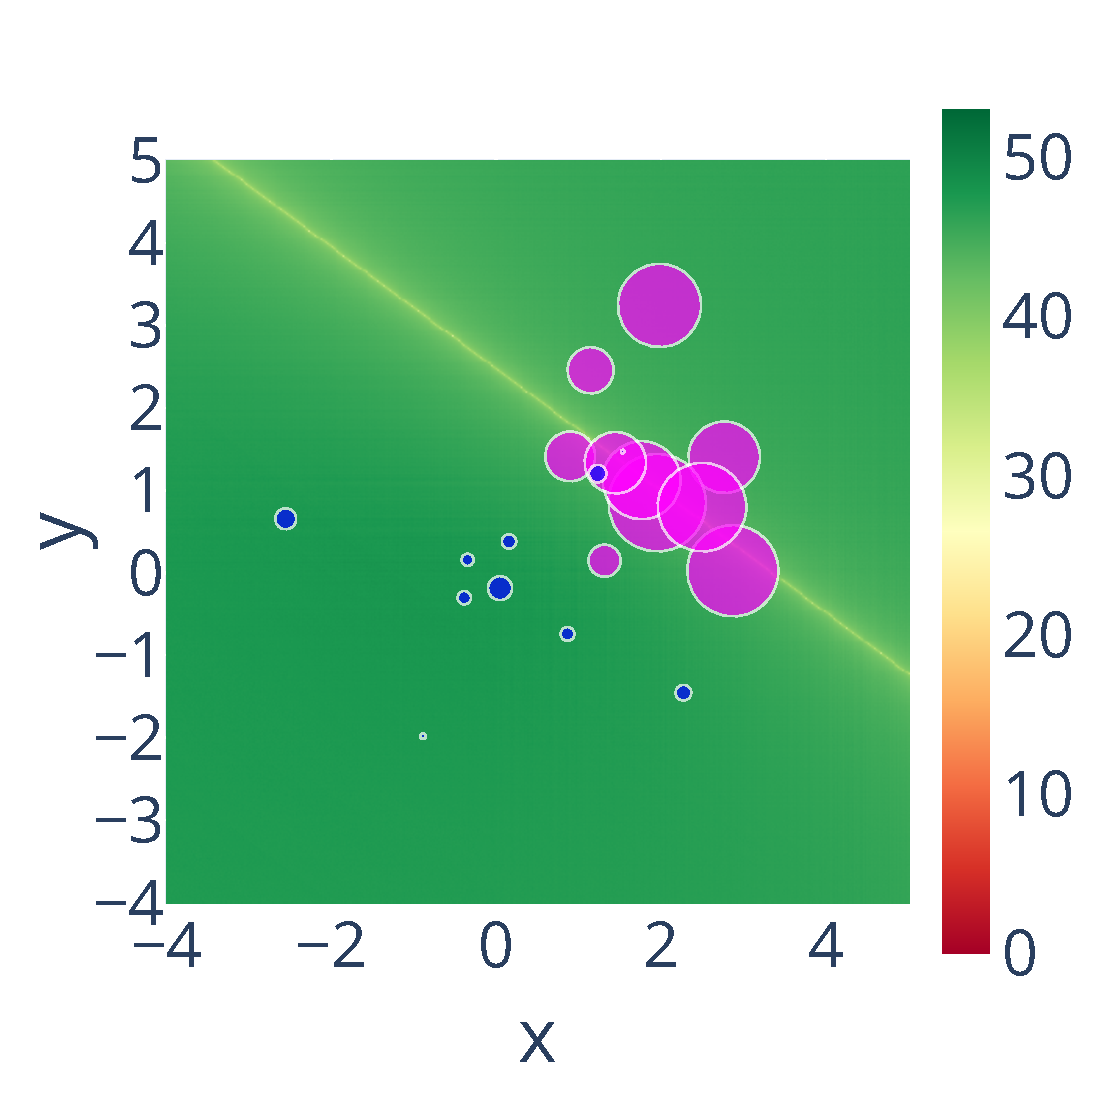
\includegraphics[width=\linewidth]{figure/Weighted/non_weighted.pdf}
        \caption{SGD weighted (non-weighted)}
        \label{fig:weighted_nw_sig}
    \end{subfigure}
    \begin{subfigure}{.45\linewidth}
        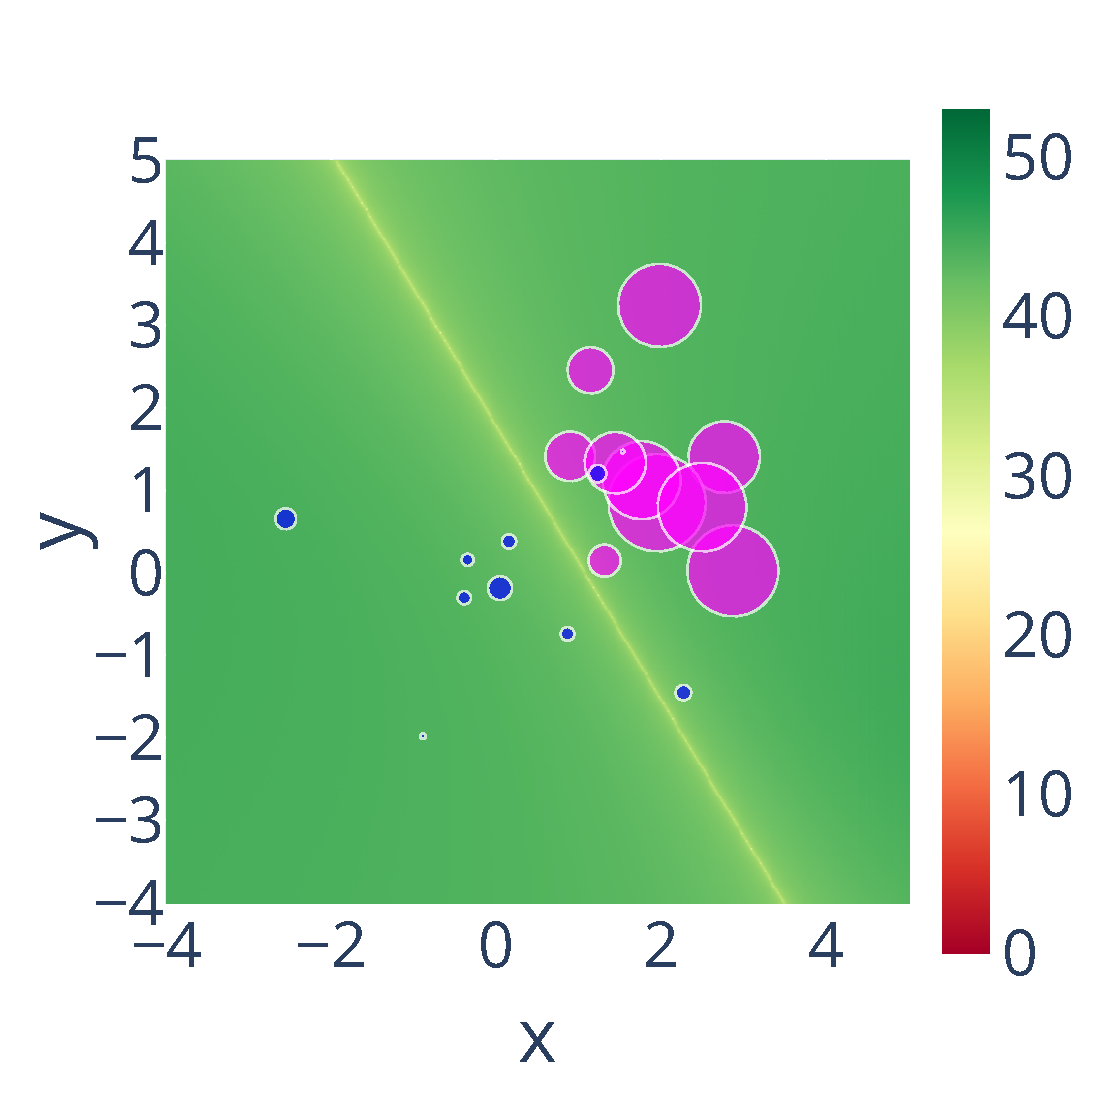
\includegraphics[width=\linewidth]{figure/Weighted/weighted.pdf}
        \caption{SGD weighted (weighted)}
        \label{fig:weighted_w_sig}
    \end{subfigure}
    \caption{
        Three examples of separating hyperplane prediction. All the figures show the number of significant bits of the prediction in RR mode. The separating hyperplane corresponds to a lower-precsion region in each figure. Using a large discretization step amplifies
        this instability.
        % respectively the results of examples    \textit{SVM} and~\textit{Weighted samples}. Figures~\ref{fig:SVM_nw_sig} and~\ref{fig:weighted_nw_sig} show the unweighted classification while Figures~\ref{fig:SVM_w_sig} and~\ref{fig:weighted_nw_sig} the classification taking into account the weights. We can see that taking into account the weight classes allows a better separation. 
        % \tristan{add labels to subfigures} \tristan{don't use this yellow for class 1, take a color that isn't in the color map. Add a legend to show the class colors.}
    }
    \label{fig:separating_hyperplan}
\end{figure}

\subsubsection{SVM}
This example uses a plain Support Vector
Classification~\cite{Platt99probabilisticoutputs} (SVC) to find the best
hyperplane separating an unbalanced dataset with two classes of 1000 and 100
points. This example tests two SVC configurations using a linear kernel with and
without a class weight parameter. The SVC predicts the class label for each
coordinate over a $[-5,5] \times [-5,5]$ grid discretized with 900 points.
Figures~\ref{fig:SVM_nw_sig} and~\ref{fig:SVM_w_sig} show the result within RR
of the classification with and without taking into account the unbalancing. We
can see that the number of significant bits is lower on the separating line and
that taking into account class imbalance allows for a better separation.

\subsubsection{SGD weighted samples}
This example uses an SGD to separate weighted points. It divides the training
set into two classes of 10 points with a bigger weight for the second class. The
SGD is trained with hyperparameters $\alpha=0.01$ and a maximum number of
iterations to 100. The prediction is made on a $[-4,5]\times[-4,5]$ grid
discretized with 250\add{,}000 points. Figures~\ref{fig:weighted_nw_sig}
and~\ref{fig:weighted_w_sig} show the number of significant bits of prediction
within RR along with dataset points in blue and \remove{violet} \add{purple}. We can see that the
separating plane corresponds to a region of lower precision, similar to the
previous examples.

% \begin{figure}
%     \centering
%     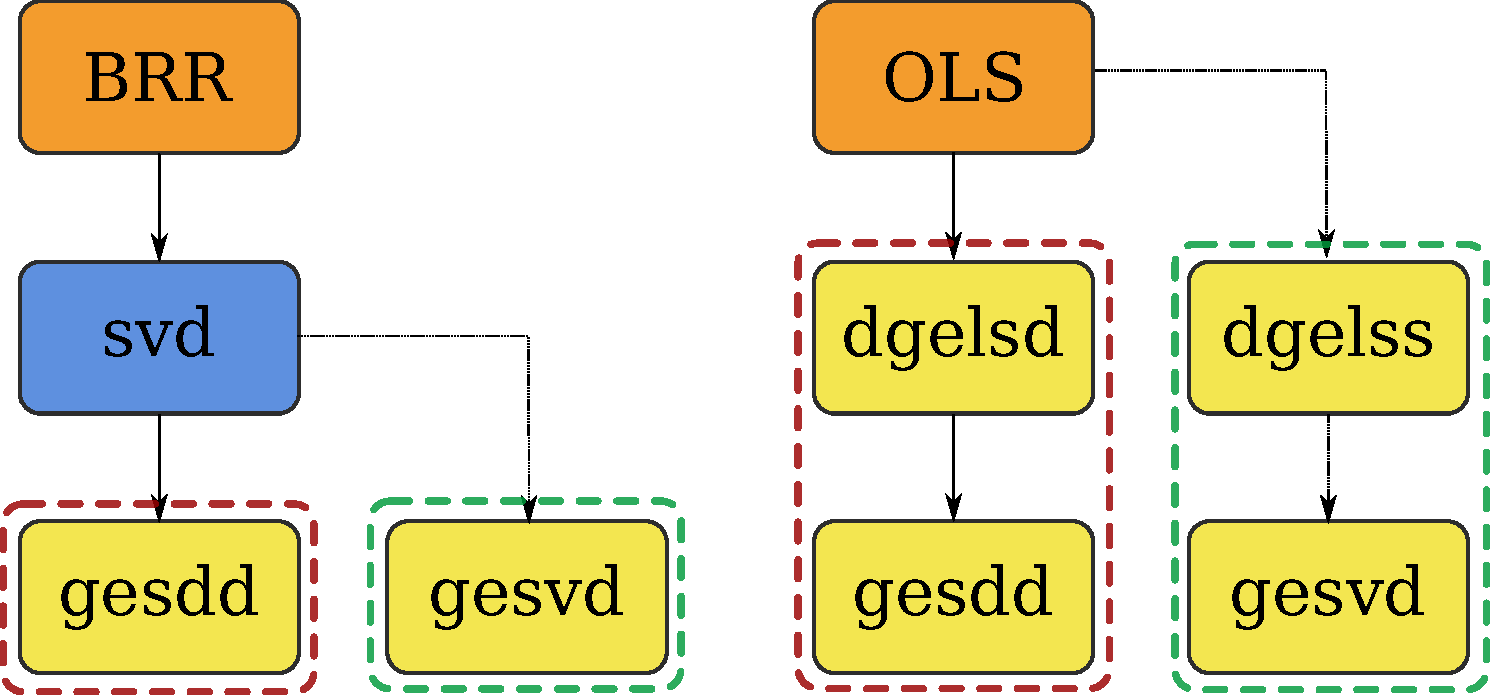
\includegraphics[width=0.5\linewidth]{figure/BRR/call_path.pdf}
%     \caption{Call paths of the Bayesian Ridge Regression (BRR) and Ordinary
%         Least Square (OLS) function. Color represents the calling library:
%         orange for scikit-learn, blue for SciPy and yellow for LAPACK. Dashed
%         color represents the original path in red and the alternative one in
%         green. Figure~\ref{fig:brr_svd_sig} shows the original method  leads to
%         numerical instabilities while the alternative one converges. }
%     \label{fig:call_path_brr}
% \end{figure}

% \begin{figure}
%     \centering
%     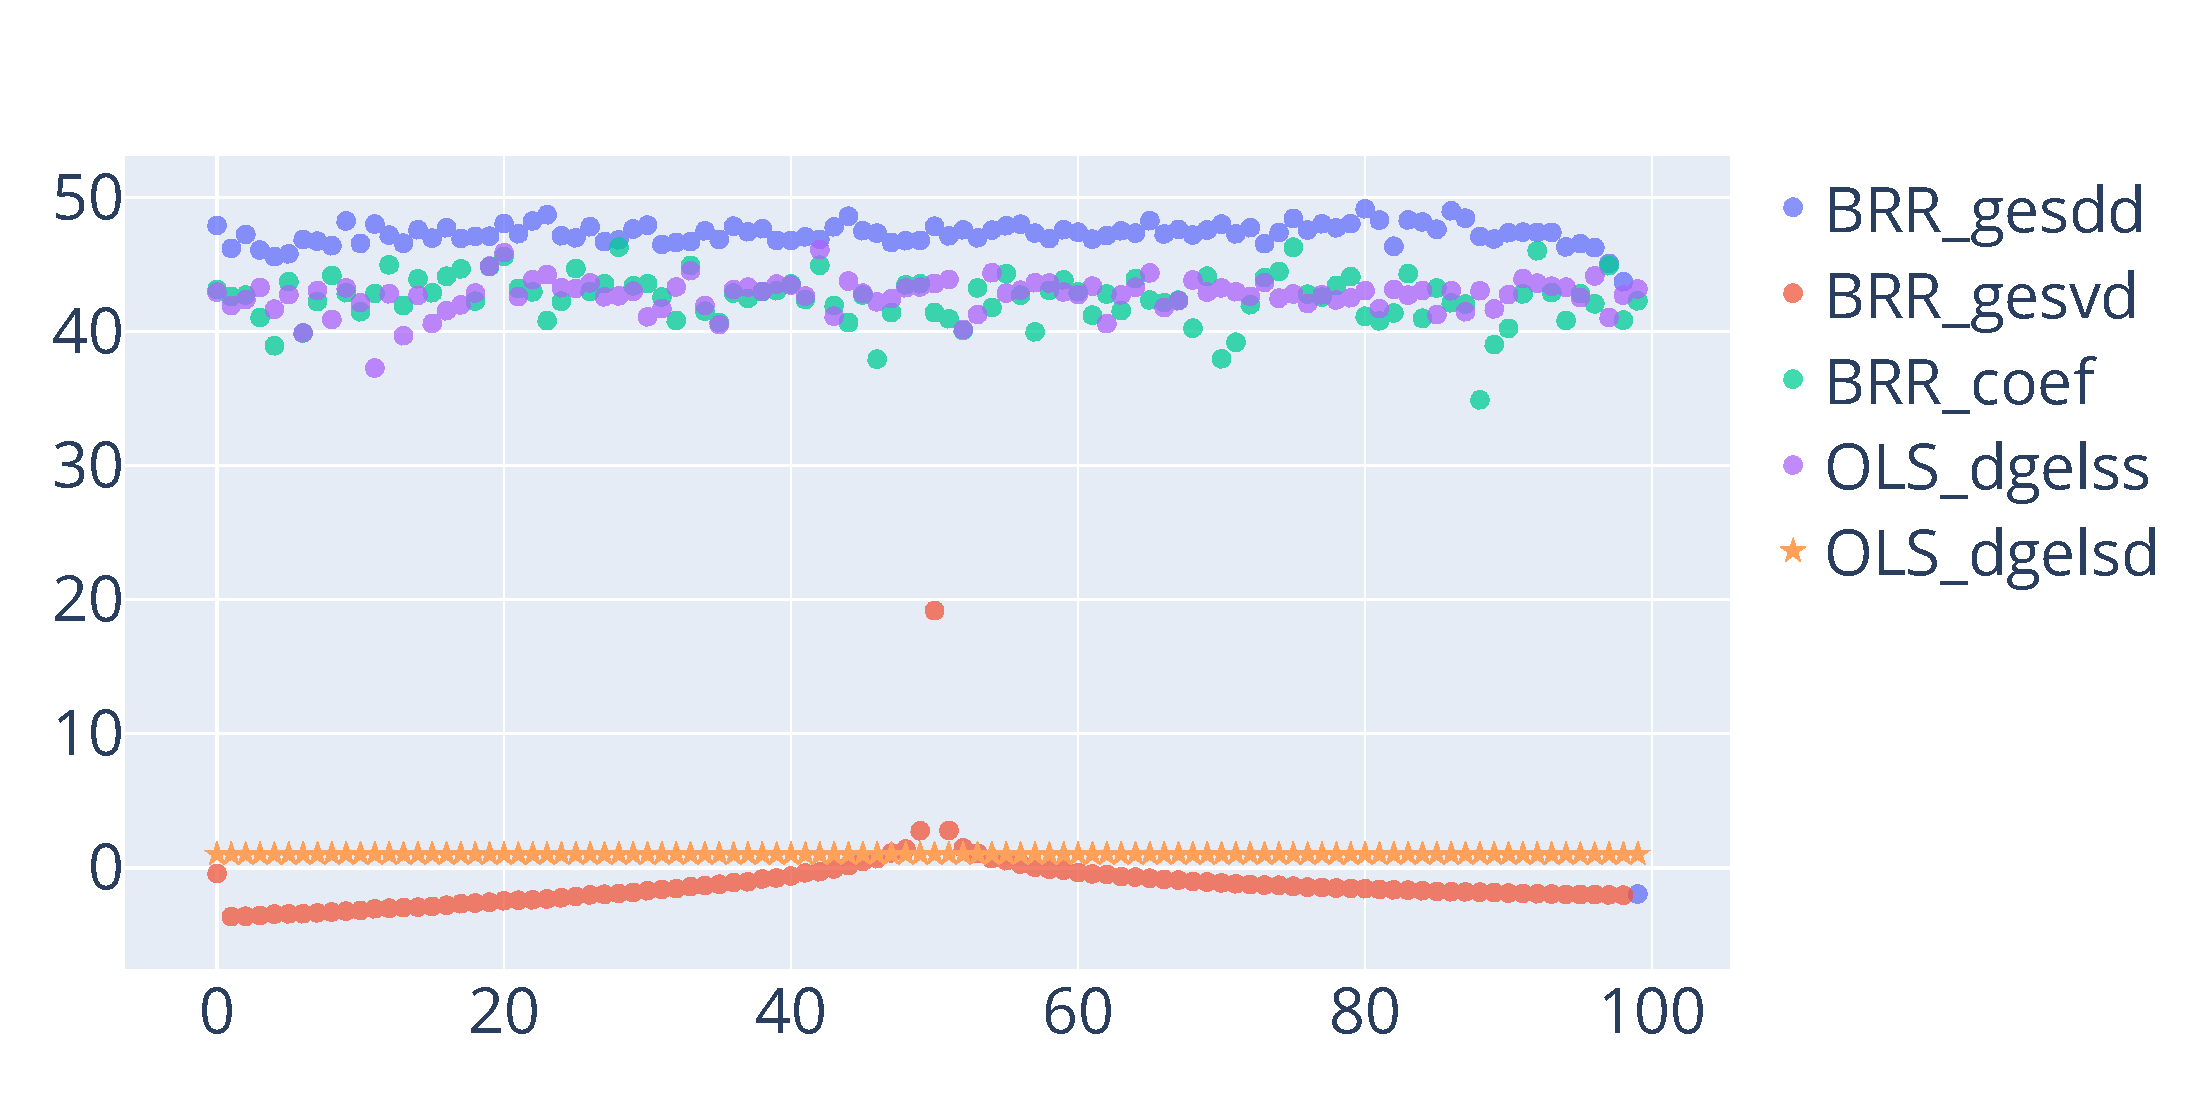
\includegraphics[width=\linewidth]{figure/BRR/BRR_coefs_sig.pdf}
%     \caption{Precision of Bayesian Ridge Regression coefficients in RR mode.
%         \texttt{BRR\_*} show the \texttt{BayesianRidge} results using the
%         \texttt{gesdd} and \texttt{gesvd} methods. \texttt{OLS\_*} show the
%         \texttt{LinearRegression} results with the \texttt{dgelsd} and
%         \texttt{dgelss} methods. The Divide \& Conquer method (\texttt{gesdd}
%         and  \texttt{dgelsd}) has low precision for \textit{BRR} and results in
%         \texttt{NaN} values (star points) for \textit{OLS}. By switching to the
%         \texttt{gesvd} method, results have a precision of 42 bits on average. }
%     \label{fig:brr_svd_sig}
% \end{figure}

% This example compares a Bayesian Ridge Regression (BRR) to the Ordinary Least
% Squares (OLS) estimator on a synthetic dataset and for one-dimensional
% regression using polynomial feature expansion. Although the example does not
% raise a runtime error, the regression coefficients computed from the fitting are
% non-significant. \pytracer traces reveal that the SVD solver used is the root
% cause for this error. Figure~\ref{fig:call_path_brr} shows the two call paths
% for BRR and OLS. The LAPACK library has two main methods for computing the SVD:
% \texttt{gesdd} and \texttt{gesvd}. The former uses a Divide \& Conquer approach,
% while the latter uses a QR decomposition. While both methods are expected to
% have the same accuracy~\cite{nakatsukasa2013stable},
% Figure~\ref{fig:brr_svd_sig} shows that \texttt{gesdd} is totally imprecise,
% with an average number of significant digits of 0\footnote{Following
%     Equation~\ref*{eq:sig-digits}, a number of significant digits below 0 means that
%     the variability ($\sigma$) is higher than the avarage value ($\mu$).} for BRR
% and even \texttt{Not-a-Number} (\texttt{NaN}) values for OLS. On the same
% figure, we can see that using the \texttt{gesvd} (\remove{dgelsd} \add{dgelss})
% method instead of the \texttt{gesdd} (\remove{dgelss} \add{dgelsd}) one, the SVD
% converges for RR and Full MCA, with a number of significant bits of 44 on
% average. This observation supports the on-going discussion among LAPACK
% developers on the instability of \texttt{gesdd} (see
% \href{https://github.com/Reference-LAPACK/lapack/issues/316}{github.com/Reference-LAPACK/lapack/issues/316}).


% that's all folks
\end{document}


